\documentclass{sty/eiiatfg}

% Hay muchos paquetes para LaTeX que facilitan centenares de trabajos
% engorrosos. Busca en Internet si no sabes hacer algo con LaTeX. El
% repositorio oficial está en https://ctan.org/

% Algunos paquetes especialmente útiles ya están incluídos en el estilo
% del TFG (consulta sty/eiiatfg.cls para más detalles).

% Cambia los datos de tu TFG en este archivo

\title{Automatización de la gestión de viviendas con carácter vacacional con Python y Raspberry Pi}
\author{Aitor Martín Martínez}

% IE = Ingeniería Eléctrica
% IEIA = Ingeniería Electrónica Industrial y Automática
% IA = Ingeniería Aeroespacial
\grado{IEIA}

% Tu número de expediente puedes consultarlo en secretaría virtual
\expediente{225553}

% En caso de múltiples directores separa los nombres con \\
% Si solo hay un tutor no pongas
\tutor{Francisco Moya Fernández}


% A partir de aquí se trata de datos opcionales. Si algún dato no quieres que figure borra la línea o coméntala poniendo el signo % al principio

% Es muy conveniente proporcionar un medio de contacto con el autor.  El correo electrónico es probablemente el menos invasivo. No uses correos con nicknames extraños, es un documento profesional. En caso de duda usa el correo de la Universidad, pero recuerda que dejará de ser válido unas semanas después de que dejes de ser alumno.
\email{aitormartin1992@gmail.com}

% No uses tu teléfono personal, será accesible para cualquier usuario de la biblioteca
\phone{925 268 800 x.3729}

% Una página web para el proyecto puede ser un requisito necesario en caso de que sea trabajo parcialmente financiado con un proyecto de I+D. Consulta a tu tutor
\homepage{https://github.com/aitormrtn/KEYHOME_PROYECT}

% Tener un repositorio GIT (http://github.com) permite llevar un control de versiones. Tu tutor puede considerarlo esencial, habla con él
\gitrepo{https://github.com/aitormrtn/KEYHOME_PROYECT}

% Pon una dirección si puede ser interesante para recibir correspondencia relacionada. No pongas tu dirección personal
\address{UCLM --- Escuela de Ingeniería Industrial y Aeroespacial\\
    Campus Universitario de la Real Fábrica de Armas}
\poblacion{Toledo}
\cpostal{45071}

% Definición de acrónimos:
% \newacronym{id}{corto}{largo}
% o bien, en versión simplificada
% \acro{corto}{largo}

% Uso de acrónimos
% \acrshort{id} nombre corto
% \acrlong{id}  nombre largo
% \acrfull{id}  nombre largo (nombre corto)
% o bien, en versión simplificada
% \acs{id} nombre corto
% \acl{id}  nombre largo
% \ac{id}  nombre larco (nombre corto)

\acro{CD}     {Compact Disc}
\acro{GNU}    {\acs{GNU} is Not Unix}
\acro{PDF}    {Portable Document Format}
\acro{TCP/IP} {Pila de protocolos de Internet}
\acro{TCP}    {Transport Control Protocol}
\acro{XML}    {eXtensible Markup Language}


% La bibliografía la puedes descomponer en varios archivos .bib
% Los archivos .bib se pueden escribir a mano con ayuda de un editor online
% (e.g. http://truben.no/latex/bibtex) o generar con Mendeley u otro
% gestor de bibliografía. Solo se incluyen las referencias que son citadas
% en el texto.
\addbibresource{bib/main.bib}
%\addbibresource{bib/how.bib}
%\addbibresource{bib/ejemplos.bib}

\fxsetup{draft,lang=spanish,theme=color,inlineface=\bfseries,marginface=\bfseries,layout={marginclue,inline,index}}

\begin{document}

% Puedes cambiar la licencia de este documento con la orden license.  Por defecto se asume Creative Commons Attribution 4.0 (ver https://creativecommons.org/licenses/by/4.0/).  
% Por ejemplo, para restringir su uso, copia y distribución:
%\license{Todos los derechos reservados.}

% Si usas muchos símbolos conviene que describas lo que significan en un archivo
% aparte (en este caso simbolos.tex).  Si no es el caso puedes comentar esta línea
\listofsymbols{simbolos.tex}

\portada
\begin{agradecimientos}
\noindent Quiero agradecerle a mi familia, especialmente a mis padres y a mi tío Javier, por haberme brindado la oportunidad de obtener una formación de calidad, ayudándome en todo momento de forma incondicional.

También quiero darle las gracias al tutor de este trabajo, Francisco Moya, por acercar el mundo de la programación a mi vida, y en general, a todos los docentes que me han acompañado en el camino, con especial atención por aquellos que sienten pasión por su trabajo y se la transmiten a sus alumnos.
\end{agradecimientos}	   
\begin{dedicatoria}
Esta obra está dedicada a la memoria de Alan Turing, cuya contribución tecnológica hace posible, entre otras muchas cosas, este trabajo de fin de grado.
\end{dedicatoria}
\begin{resumen}

\noindent Desde hace ya varios años, el auge de empresas tecnológicas asociadas al alquiler vacacional, como Booking\footnote{\url{https://www.booking.com/}} o Airbnb\footnote{\url{https://www.airbnb.es/}}, han propiciado un cambio significativo en la manera que funciona el turismo, dando la oportunidad, tanto a profesionales del sector como a principiantes, de tener visibilidad ante clientes potenciales.

Es un hecho que muchas personas han hecho de este modelo su forma de ganarse la vida, dedicándole a esta tarea su jornada laboral, a tiempo parcial o completo, para gestionar una o varias viviendas de uso turístico. Algunas de las tareas que se desempeñan en estos puestos de trabajo son las siguientes:
\begin{itemize}
\item Actualizar los precios en función de la demanda.
\item Responder las dudas a los clientes.
\item Ofrecer acceso a la vivienda y atender a los usuarios en su llegada.
\item Gestionar los trabajos de limpieza.
\item Prevenir el exceso de ventas para una misma habitación en el mismo día cancelando la disponibilidad de una misma vivienda en distintas plataformas.
\end{itemize}

\noindent En la actualidad existen herramientas que permiten actualizar los precios de forma automática en base a algoritmos que tienen en cuenta la demanda, y también pueden encontrarse algunas que permiten sincronizar los calendarios de las distintas plataformas entre sí, con el fin de facilitar el trabajo de los propietarios de viviendas de uso turístico.

El objeto de este trabajo de fin de grado consiste en gestionar la llegada del cliente a la vivienda de uso turístico, haciendo que las tareas desempeñadas entre el momento en que se realizan las reservas, y el que los clientes acceden a la vivienda, queden completamente automatizados, liberando de esta manera una importante carga de trabajo a los propietarios. El resultado de este trabajo es hacer que el anfitrión de la vivienda de uso turístico pueda tener la garantía de que su negocio se está gestionando de forma automática, y que solo se le avisará en casos particulares, cuando sea estrictamente necesario.

Para llevar a cabo esta tarea se creará un sistema que permita gestionar, de forma automática, por medio de una Raspberry Pi Zero W, la apertura de las puertas de acceso a la vivienda en los momentos que proceda. De igual manera, se integrarán en el sistema todas aquellas tareas que pueden tenerse en cuenta, como las posibles cancelaciones, la organización de los equipos de limpieza o las medidas de seguridad que garantizarán la tranquilidad de aquellos anfitriones que deseen hacer uso de este sistema.

Tanto los usuarios finales, como el administrador, podrán hacer uso de todas estas herramientas a partir de la aplicación de mensajería instantánea "Telegram". La elección de Telegram como aplicación de la plataforma no es casual, si no que responde a unos criterios bien definidos:
\begin{itemize}
\item Telegram es, y siempre ha sido, una aplicación de código abierto, lo cual abre la puerta a posibilidades infinitas de programación, así como la seguridad de saber que el sistema será estable en relación a las políticas de la plataforma. 
\item La inmensa mayoría de la población vive familiarizada con las aplicaciones de mensajería instantánea, por lo que la curva de aprendizaje sería mínima, y ello aceleraría considerablemente la adaptación de los clientes potenciales.
\item Telegram trabaja con un cifrado de 64 bits, de extremo a extremo, en todas sus comunicaciones. Esto facilita considerablemente el trabajo y resulta de gran utilidad a la hora de evitar interceptaciones de información por parte de terceros.
\end{itemize}
\end{resumen}

\begin{abstract}
\noindent For several years now, the rise of technology companies associated with vacation rental, such as Booking\footnote{\url{https://www.booking.com/}} or Airbnb\footnote{\url{https://www.airbnb.es/}}. They have brought about a significant change in the way tourism works, giving professionals, as well as beginners, the opportunity to have visibility before potential clients.

It is a fact that many people have made this model their way of earning a living, dedicating their part-time or full-time workday to this task to manage one or more houses for tourist use. Some of the tasks performed in these jobs are the following:
\begin{itemize}
\item Update prices based on demand.
\item Answer questions to customers.
\item Offer access to housing and attend to users upon arrival.
\item Manage cleaning jobs.
\item Prevent excess sales for the same room on the same day by canceling the availability of the same home on different platforms.
\end{itemize}

\noindent Currently there are tools that allow updating prices automatically based on algorithms that take into account demand, and there are also some that allow synchronizing the calendars of the different platforms with each other, in order to facilitate the work of homeowners for tourist use.

The purpose of this final degree project is to manage the client's arrival at the dwelling for tourist use, making the tasks performed between the time the reservations are made and the clients accessing the dwelling completely automated, thus relieving a significant workload for owners. The result of this work is to ensure that the host of the tourist-use dwelling can have the guarantee that his business is being managed automatically, and that he will only be notified in particular cases, when strictly necessary.

To carry out this task, a system will be created that automatically manages, by means of a Raspberry Pi Zero W, the opening of the access doors to the house at the appropriate times. Likewise, all those tasks that may be taken into account, such as possible cancellations, the organization of cleaning teams, or security measures that will guarantee the tranquility of those hosts who wish to use this system, will be integrated into the system.

Both end users and the administrator will be able to make use of all these tools from the "Telegram" instant messaging application. The choice of Telegram as application of the platform is not accidental, if not that it meets well-defined criteria:
\begin{itemize}
\item Telegram is, and always has been, an open source application, which opens the door to infinite programming possibilities, as well as the security of knowing that the system will be stable in relation to the platform's policies.
\item The vast majority of the population lives familiarized with the applications of instantaneous mail, reason why the learning curve would be minimal, and this would accelerate considerably the adaptation of the potential clients.
\item Telegram works with 64-bit encryption, end-to-end, in all its communications. This considerably facilitates the work and is very useful in avoiding interception of information by third parties.
\end{itemize}
\end{abstract}


\indices
%Poniendo \if0 hacemos que los puntos que haya debajo no se compilen
%\fi %% fin de \if0 A partir de aquí el \if0 ya no tendría efecto
% Para incluir un fragmento basta sustituir el \if0 por \if00 (un cero más).

% El cuerpo del documento está en la carpeta tex
% Aquí simplemente se incluyen los archivos correspondientes a cada capítulo.

% No los llames capitulo1, capitulo2, etc. Los números los pondrá LaTeX según
% el orden en que los pongas.  Eso facilitará después su posible reordenación
% o división.

% Esta estructura corresponde a un documento científico-técnico.
% Si ves que tu proyecto concuerda con un trabajo profesional organiza el 
% documento según UNE 157001

\if00
\chapter{Introducción} 
\label{ch:introduccion}

\section{Presentación del problema} 
\label{sec:presentacion-del-problema}

\noindent El alquiler de viviendas para uso turístico constituye, sin lugar a dudas, un pilar para el turismo, y por tanto, para la economía en España. El turismo es el sector que más riqueza aporta a la economía española, en términos de producto interior bruto (PIB) y de empleo \cite{hosteltur2020}. No obstante, la integración de sistemas de automatización que tienen por objeto recibir a los clientes en este sector, no alcanza la misma velocidad, ya que en la mayoría de casos se sigue atendiendo a los turistas con el mismo modelo de hace 10 o 15 años.

La mayoría de las viviendas de uso turístico siguen requiriendo una considerable carga de trabajo para sus anfitriones, y lejos de convertirse en un ingreso pasivo, se transforma en un trabajo que requiere atender una por una las nuevas reservas, recibir a los clientes, gestionar al personal de limpieza, responder ante posibles desperfectos, etc. Todo esto hace que muchas personas recurran a alquilar sus viviendas de la forma tradicional, por medio de particulares que harán uso de la misma durante un largo periodo de tiempo, a cambio de un monto inferior al que se recaudaría, en muchas ocasiones, por medio del alquiler turístico.

Un sistema automatizado será capaz, por su naturaleza, de ofrecer servicios más económicos, o de mayor calidad, ya que su costé se verá reducido de forma considerable, y permitirá convertir estos ingresos en pasivos para los propietarios, quienes verán reducida de forma considerable su carga de trabajo, y esto les motivará a formar parte de esta actividad.

Además, esto también jugará a favor de la economía de nuestro país, ya que en las fechas de mayor ocupación podrá tener disponibilidad de un mayor número de plazas para pernoctar, con todos los beneficios que ello implica a nivel económico.

\section{Soluciones propuestas} 
\label{sec:soluciones-propuestas}

\noindent Este trabajo de fin de grado pretende introducir los desarrollos tecnológicos actuales en el mundo de las viviendas de uso turístico, eliminando parte de la carga de trabajo a la que se enfrentan los anfitriones de dichas viviendas. Algunas de las actividades que se pretenden realizar son las siguientes:
\begin{itemize}
\item Atención automatizada del cliente. El anfitrión de la vivienda no tendrá porque saber si alguien ha hecho o no una reserva si no quiere. Este sistema atenderá al cliente en el momento en que realice una reserva, y lo guiará hasta la vivienda, donde se encargará también de ofrecerle acceso.
\item Automatización de las cancelaciones. En caso de que se produzcan cancelaciones, el sistema lo tendrá en cuenta y gestionará debidamente las acciones pertinentes, con el fin de anular el acceso para la persona que ejecuta la cancelación y abrirlo a nuevos clientes potenciales.
\item El proyecto incluirá un panel de administración para el anfitrión, desde el cuál podrá realizar las siguientes tareas:
\begin{itemize}
\item Consultar las reservas existentes. El anfitrión tendrá la posibilidad de consultar todas las reservas que contenga el sistema.
\item Crear nuevas reservas. El anfitrión podrá crear reservas para los días que considere convenientes, desde un panel de gestión implantado en la propia aplicación de Telegram.
\item Anular reservas. De igual manera, el anfitrión tendrá la posibilidad de cancelar aquellas reservas que considere convenientes.
\item Por último, el panel de administración para el anfitrión incluirá la posibilidad de realizar la apertura de las puertas de forma automática.
\end{itemize}
\end{itemize}
Para llevar a efecto la apertura de las puertas se hará uso de una Raspberry Pi Zero W\footnote{\url{https://www.raspberrypi.org/products/raspberry-pi-zero-w/}}. Esta placa, por medio de su programación interna, facilitará la activación del circuito eléctrico que permitirá realizar la apertura de puertas. Además, gestionará la ejecución de todos los programas que se mencionan en el presento proyecto.

En cuanto al uso de Telegram como plataforma de mensajería instantánea, se hará uso de la libreria disponible en python, \emph{PyTelegramBotApi}\footnote{\url{https://github.com/python-telegram-bot/python-telegram-bot}}.

Los programas que se ejecutan trabajan con el envío y la recepción de correos electrónicos, por medio de los cuales realizan la automatización de los procesos. Estos correos electrónicos se enviarán a partir del lenguaje de programación Python con la libreria \emph{smtplib}\footnote{\url{https://github.com/python/cpython/blob/master/Lib/smtplib.py}}.

\section{Organización de la memoria} 
\label{sec:organizacion-memoria}

\noindent La organización de este documento responde a un documento científico-técnico. Se descompone en los siguientes capítulos.

\begin{description}
    \item[\autoref{ch:objetivos}] Enumera y justifica los objetivos del proyecto y establece los límites intrínsecos y extrínsecos de ejecución del TFG.
    \item[\autoref{ch:antecedentes}] Analiza los antecedentes y estado del arte en relación al tema del proyecto.
    \item[\autoref{ch:desarrollo}] Describe todo el proceso de desarrollo del TFG.  Esto incluye la metodología de trabajo empleada y las diferentes etapas o iteraciones que se han llevado a cabo.  No dudes en descomponer el capítulo en varios si aglutina demasiado material.
    \item[\autoref{ch:resultados}] Describe en detalle los resultados obtenidos y las pruebas realizadas. Discute los resultados en relación a los objetivos del proyecto.
    \item[\autoref{ch:conclusiones}] Recopila las principales conclusiones del proyecto y comenta las líneas de trabajo futuro, en caso de que se contemplen.
    \item[\deschyperlink{ch:anexos}{Anexos}] Complementan la información del cuerpo del documento con información técnica útil para reproducir los resultados, pero innecesaria para comprender en su totalidad el TFG realizado.
    \item[\deschyperlink{ch:bibliografia}{Bibliografía}] Recopila las referencias bibliográficas utilizadas en este documento.
\end{description}

\section{Repositorio de información}
\label{sec:repositorio}

\noindent El material generado durante la ejecución de este proyecto está disponible en el repositorio \thegitrepo{}. El material incluye el código \LaTeX{} del presente documento, el código fuente de los programas realizados o modificados, y todos los datos generados en la evaluación de resultados.
\fi

\if00
\chapter{Objetivos}
\label{ch:objetivos}

\noindent El objeto principal de este trabajo de fin de grado es el de automatizar por completo la recepción de los turistas en las viviendas de uso turístico, de manera que los propietarios de las mismas no tengan que dedicar su tiempo a esta tarea. Para la llevar a cabo esta empresa, el objetivo principal se desglosa en otros más pequeños que trabajarán en conjunto. A continuación se identifican y explican cada uno de los objetivos que se han considerado:

\section{Circuito electrónico capaz de abrir una cerradura eléctrica} 
\label{sec:circuito-electronico-capaz-de-abrir-una-cerradura-electrica}

\noindent Para poder abrir la puerta a los clientes en su llegada, es necesario que el circuito sea capaz de abrir la puerta. Este objetivo se alcanzará una vez que, a partir de una señal de 3 voltios emitida por la Raspberry Pi Zero W, se proceda a activar la apertura de una cerradura eléctrica. Para ello se hará uso de los materiales que resulten convenientes, como relés, transformadores, cableado, etc.

\section{Programa para apertura de la vivienda desde Telegram} 
\label{sec:programa-que-atienda-las-peticiones-de-apertura-desde-telegram}

\noindent El presente objetivo estará completado en el momento en que el turista, al llegar a la vivienda de uso turístico, tenga la posibilidad de realizar la apertura de la vivienda desde la aplicación de Telegram.

\section{Panel de administración desde Telegram} 
\label{sec:creacion-de-un-panel-de-administracion-desde-telegram}

\noindent Como administrador, la persona o personas que gestionen la vivienda tendrán la posibilidad de realizar distintas actividades desde la propia plataforma de Telegram. Este objetivo se habrá alcanzado en el momento en que, por medio de un programa integrado en la Raspberry Pi, el administrador sea capaz de realizar las siguientes operaciones:

\begin{itemize}
\item Consultar las reservas existentes. El anfitrión tendrá la posibilidad de consultar todas las reservas que contenga el sistema.
\item Crear nuevas reservas. El anfitrión podrá crear reservas para los días que considere convenientes, desde un panel de gestión implantado en la propia aplicación de Telegram.
\item Anular reservas. De igual manera, el anfitrión tendrá la posibilidad de cancelar aquellas reservas que considere convenientes.
\item Por último, el panel de administración para el anfitrión incluirá la posibilidad de realizar la apertura de las puertas de forma automática.
\end{itemize}

\section{Automatización de nuevas reservas} 
\label{sec:automatizacion-de-nuevas-reservas}

\noindent Con el fin de que el propietario de la vivienda de uso turístico pueda automatizar el proceso de atención de los clientes, la Raspberry Pi integrará un programa  en el que se gestionarán todas las nuevas reservas que se produzcan de la vivienda, de manera que permitirá la entrada a los clientes una vez que estos se identifiquen a través de su número de reserva.

\section{Automatización de cancelaciones de reservas} 
\label{sec:automatizacion-de-cancelaciones-de-reservas}

\noindent En la mayoría de plataformas de alquiler vacacional, como Booking, Airbnb, Homeaway, etc. Los clientes tienen la posibilidad de realizar cancelaciones. Por lo tanto, esto es algo que se debe tener en cuenta a la hora de automatizar el proceso de reservas y recepción de clientes. Para tal efecto se integrará un programa en la Raspberry Pi que recibirá las cancelaciones de los clientes, y lo incluirá en el sistema, de manera que esas personas no tendrán acceso a la vivienda por medio del número de reserva que obtuvieron antes de su cancelación.

\section{Diseño en tres dimensiones para contener el circuito} 
\label{sec:creacion-de-un-diseño-en-tres-dimensiones-para-contener-el-circuito}

\noindent Con el fin de mejorar la seguridad del sistema, así como su aspecto visual, se procederá a crear un diseño en tres dimensiones donde se contendrá todo el circuito electrónico.

Este diseño deberá permitir su instalación en la pared, por medio de tornillería o por medio de adhesivos, y proporcionará una sujeción firme de los elementos que se encuentren en su interior.

También integrará la posibilidad de incluir un candado que asegure su cierre, de manera que se trate de evitar la manipulación indeseada por parte de otros usuarios.


\section{Sistema de alarma ante posibles manipulaciones} 
\label{sec:sistema-de-alarma-ante-posibles-manipulaciones}

\noindent Todas las medidas de seguridad que se tomen serán de gran ayuda para crear confianza en aquellos propietarios que quieran hacer uso de este sistema. Si la Raspberry Pi trabajase de forma manipulada por algún usuario malintencionado, podría significar un problema importante de seguridad. Es por ello que se integrará en la placa un programa que permitirá advertir al administrador principal, por medio de un correo electrónico, en caso de que alguien haya abierto la caja donde se encuentra. De esta manera se le permitirá conocer la situación y actuar en consecuencia.

\section{Sistema de alarma ante interrupciones} 
\label{sec:sistema-de-alarma-ante-interrupciones}

\noindent Un apagón, una caída de internet o un fallo interno de la Raspberry Pi, podrían provocar en un momento determinado una interrupción en el trabajo de la misma. Para que el administrador principal pueda ser conocedor de ello, y actuar en consecuencia, se incluirá un programa con el que se le avisará de lo sucedido a través de un correo electrónico.

\fi

\if00
\chapter{Motivación y antecedentes}
\label{ch:antecedentes}

\noindent Año tras año, en todos los países occidentales, el modelo de negocio de las plataformas de alquiler vacacional con apartamentos turísticos no deja de crecer \cite{juanjocerezo2018}. La forma en la que se organizan las vacaciones, los viajes de negocios y cualquier actividad que incluya pernoctar, está adaptándose a una nueva forma de economía colaborativa. La repercusión que esto tiene en el mercado es positiva, haciendo que nuestro país vea aumentada su capacidad para acoger turistas, de forma que el producto interior bruto recibe un fuerte impulso.\\
No obstante, este modelo de economía colaborativa no está al acceso de todo el mundo, ya que la atención de los clientes es algo que requiere una importante inversión de tiempo, que no siente resulta compatible con la vida laboral o personal de los potenciales anfitriones.\\
Algunos de los problemas que requieren de la atención y el tiempo de los propietarios de viviendas de uso turístico, han sido automatizados por empresas que, a cambio de tarifas mensuales o anuales, ofrecen diferentes servicios a los clientes:
\begin{itemize}
\item Evitar un exceso de huéspedes para una misma habitación. La mayoría de los propietarios de viviendas de uso turístico, tienen sus anuncios en varias plataformas, como Airbnb, Booking, Homeaway, etc. Esto puede provocar que diferentes personas alquilen la misma propiedad en idénticas fechas, produciendo así un fenómeno de sobre venta, lo cual resulta castigado en la mayoría de los casos por medio de sanciones en dichas plataformas. Para solucionar este problema, las estas plataformas ofrecen ya soluciones\footnote{\url{https://www.airbnb.es/help/article/99/como-sincronizo-mi-calendario-de-airbnb-con-otro-calendario}}, pero además existen múltiples empresas que permiten sincronizar los calendarios, haciendo que al recibir una reserva en una plataforma, las demás queden deshabilitadas para tales fechas, acabando así con este indeseado fenómeno.
\item Responder a los clientes. La mayoría de plataformas de alquiler vacacional, incluyen en su software la posibilidad de ofrecer respuestas automáticas\footnote{\url{https://partner.booking.com/es/ayuda/reservas/}}, de manera que los propietarios de las viviendas no se vean obligados a responder uno por uno a los clientes.
\item Apertura de puertas de forma automática. Existen además empresas que se dedican a implantar sistemas automáticos para la apertura de puertas\footnote{\url{https://raixer.com/funcionamiento/abrir-puertas-automaticamente/}}. Estas aperturas se realizan a través de una petición de usuario, bien por medio de una llamada telefónica, o bien por medio de una aplicación que se puede descargar en Android e iOS.
\item Cálculo automatizado de precios. Optimizar los precios de una vivienda turística puede resultar un auténtico quebradero de cabeza para aquellos que quieran hacerlo de forma acertada. Las grandes cadenas hoteleras funcionan por medio de algoritmos automatizados que actualizan constantemente los precios en función de muchas variables, como la demanda, el tiempo restante, etc. En la actualidad, existen también plataformas que permiten actualizar dichos precios de forma automatizada\footnote{\url{https://hello.pricelabs.co/}}, de manera que el propietario, a cambio de un pago mensual, pueda ahorrarse una cantidad considerable de tiempo y potenciar al máximo la optimización de sus precios.

\end{itemize}

\noindent Como puede observarse, las empresas tecnológicas han apostado por el mercado de los alojamientos turísticos para emprender negocios, optimizando cada vez más esta forma de comercio. Sin embargo, los anfitriones siguen contando con una importante carga de trabajo, que repercute en su capacidad de incorporarse a este modelo de economía colaborativa.

Las motivaciones principales de este trabajo de fin de grado pasan por mejorar, de manera bidireccional, la experiencia de los huéspedes y los anfitriones, así como acercar a estos últimos la posibilidad de poder incluir este modelo de negocio pasivo en su economía personal. A continuación se mencionarán algunas de estas motivaciones de manera más detallada.

\section{Automatización completa del proceso de reserva} 
\label{sec:automatizacion-completa-del-proceso-de-reserva}

\noindent La posibilidad de incluir un sistema automatizado por completo, o uno semi automatizado, puede ser decisiva a la hora de que una persona se decida por el modelo de negocio de las viviendas de uso turístico.

El trabajo y los asuntos personales suelen requerir de una cantidad importante de recursos para las personas, que no siempre disponen del tiempo y la energía suficiente para atender a los turistas, y debido a ello, deciden abandonar este tipo de inversiones.

Este aspecto podría ser distinto, sin embargo, si por medio de un sistema automatizado, el anfitrión pudiera tener la tranquilidad de saber que su negocio se está gestionando solo, ya que de esta manera si podría plantearse esta inversión sabiendo que no le requerirá invertir tiempo de forma diaria. Un sistema que atienda de principio a fin al cliente, organizando cada reserva y ofreciendo el acceso a la vivienda, podría dar una solución definitiva a este problema y, de esta manera, abrir este terreno a multitud de potenciales anfitriones.

\section{Uso de aplicaciones de mensajería instantánea} 
\label{sec:uso-de-aplicaciones-de-mensajeria-instantanea}

\noindent En la actualidad, recientes estudios \cite{itreseller2019} afirman que el 85 por ciento de los españoles utiliza aplicaciones de mensajería instantánea. Para cualquier modelo de negocio, incluir una nueva tecnología en la que la curva de aprendizaje sea mínima, tendrá siempre un impacto positivo en la supervivencia de su fase inicial. En este caso, hacer que todo este sistema se automatice por medio de aplicaciones de mensajería instantánea hará que se facilite su uso a la inmensa mayoría de la población.

Además, según un estudio \cite{samuelfernandez2019} realizado por Telefónica, se ha demostrado que el 95,1\% de los españoles prefiere enviar un mensaje a realizar una llamada, por lo que se demuestra, una vez más, la validez de este método como forma de gestión de estos negocios al alza.

\section{Estado del arte}

\noindent El internet de las cosas, según Wikipedia\footnote{\url{https://es.wikipedia.org/wiki/Internet_de_las_cosas}} se define como la interconexión digital de objetos cotidianos por internet.

Su principal objetivo es el de facilitar la vida de las personas, evitando tener que hacer una importante cantidad de trabajos manuales, y en muchas ocasiones, optimizando los resultados obtenidos respecto a un humano.

\subsection{Historia del internet de las cosas}

\noindent Como todo avance tecnológico, el internet de las cosas establece su base a partir de otras tecnologías que lo precedieron antes y permitieron su evolución. Es por ello que, a la hora de hacer un análisis histórico, marcar el comienzo es un proceso que implica siempre cierto grado de subjetividad.

En este caso, se establece en 1969 el comienzo del internet de las cosas con el origen del propio internet, año en el que se realizó por primera vez la red operativa ARPANET\cite{tibipuiu2020}. Sin embargo, no fue hasta 1999 cuando, Kevin Asthon, acuñó por primera vez el concepto de internet de las cosas mientras impartía una conferencia en Procter and Gamble.

Tras este suceso, el término empieza a ser más extendido en diversos medios de comunicación, dando lugar durante estos primeros años del siglo XXI al uso de la tecnología RFID\cite{sorayapa2012}, cuyo propósito fundamental es la de transmitir información de los objetos a través de ondas de radio.

El año 2005 supone un año de suma importancia para el internet de las cosas, ya que es el momento en que la agencia de las naciones unidas "International Telecomunications Union (ITU)" reconoce esta materia haciendo público su primer estudio sobre el tema. Adicionalmente, ese año aparece por primera vez Arduino, un tipo de computadora orientada a la detección y control de objetos cotidianos.

Con el fin de hacer una base estable y estandarizada sobre esta materia, en el año 2008 un grupo de empresas importantes se unen para crear IPSO\footnote{\url{https://es.wikipedia.org/wiki/Internet_de_las_cosas}}, con el fin de promover el uso de un protocolo de internet en los objetos inteligentes.

En 2009 se crea la fundación Raspberry Pi\cite{rubenandres2019}, como una asociación caritativa que es regulada por la comisión de caridad de Inglaterra y Galés. Estas computadoras potenciarán activamente a partir de entonces, junto con arduino y otras muchas, la evolución y extensión del internet de las cosas.

En 2010, el número de objetos cotidianos y dispositivos conectados a internet superaba los 12 mil millones\cite{daveevans2011}.

En 2020, se estima que la cantidad de objetos conectados a internet ascenderá a 34 mil millones\cite{martinfernandez2017}.

\subsection{Historia de Raspberry Pi}

\noindent Los primeros diseños de Raspberry pi se efectuaron en el año 2006. Sin embargo, no fue hasta 2009 cuando apareció la fundación Raspberry Pi, dando así una figura estable a la imagen de esta marca. La finalidad de esta iniciativa era la de hacer que los niños aprendieran informática, tal como lo describió el administrador de esta fundación, Eben Upton.

\subsubsection{Raspberry Pi 1 modelo A}

\noindent El primer modelo de Raspberry Pi fue la Raspberry Pi 1 modelo A, la cual apareció en 2012 y contaba ya con 26 conectores GPIO, salida de vídeo HDMI, vídeo RCA, conector Jack, con un procesador Broadcom BCM2835 de 700MHZ y una memoria RAM de 256MB. Puede observarse gráficamente este modelo en la figura~\ref{fig:raspberry-pi-1-modelo-a}.

\begin{figure}[tbp]
\centering
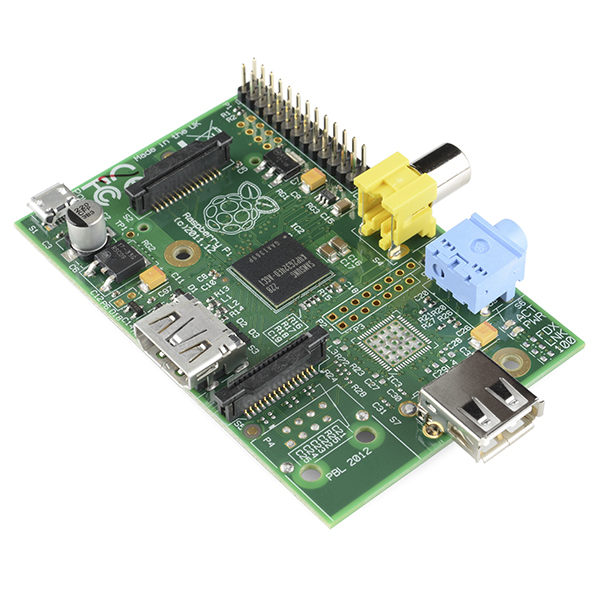
\includegraphics[scale = 1.5]{fig/Raspberry-Pi-1-modelo-A.jpg}
\caption{Raspberry Pi 1 modelo A}
\label{fig:raspberry-pi-1-modelo-a}
\end{figure}

\subsubsection{Raspberry Pi 1 modelo B}

\noindent También en 2012, la Raspberry Pi 1 modelo B apareció en el mercado trayendo el doble de memoria RAM que su predecesora, hasta los 512MB. Adicionalmente, también se le añadió un puerto USB más, y un conector RJ-45. Más tarde apareció el modelo B+, que incluía 4 puertos USB y usaba una tarjeta MicroSD, en lugar de la SD.

\subsubsection{Raspberry Pi 2 modelo B}

\noindent No fue hasta 2014 cuando hizo su aparición el siguiente modelo, la Raspberry Pi 2 modelo B, que cambió por primera vez el procesador de sus predecesoras, incorporando uno de 4 núcleos y aumentando su frecuencia hasta los 900MHz. La memoria RAM ascendió al doble de capacidad, llegando hasta 1GB. Además de todo eso, esta Raspberry Pi incluyó 40 pines GPIO y eliminó la conexión RCA. En la figura~\ref{fig:raspberry-pi-2-modelo-B} se muestra este modelo de Raspberry Pi.

\begin{figure}[tbp]
\centering
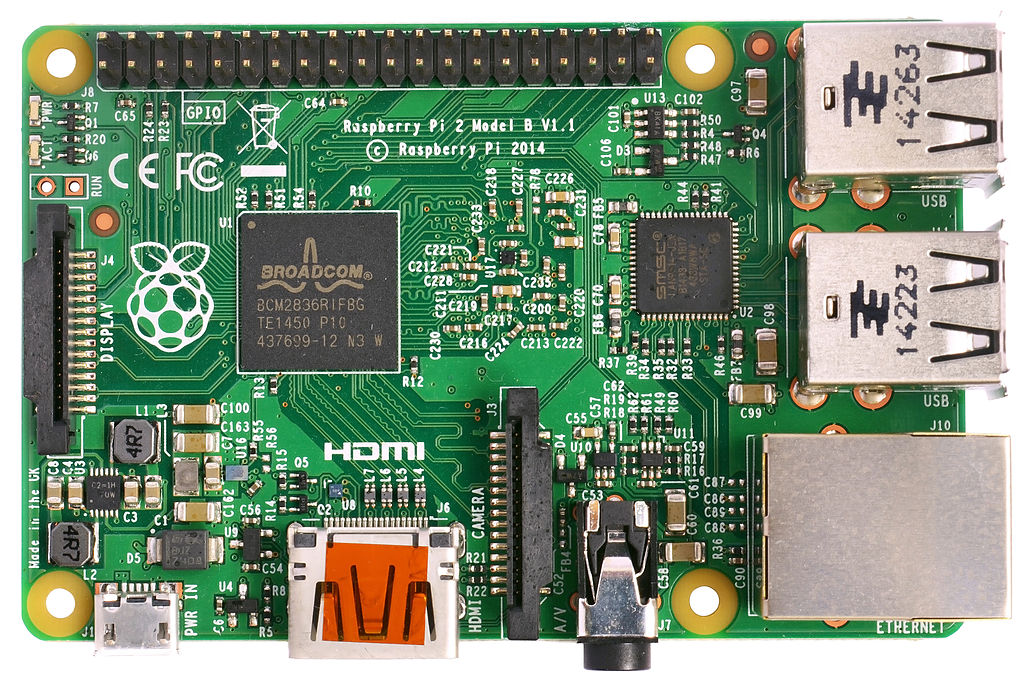
\includegraphics[scale = 1]{fig/Raspberry-Pi-2-modelo-B.jpg}
\caption{Raspberry Pi 2 modelo B}
\label{fig:raspberry-pi-2-modelo-B}
\end{figure}

\subsubsection{Raspberry Pi 3 modelo B}

\noindent Con nacimiento en 2016, la Raspberry Pi 3 modelo B llegó con un procesador nuevo y mejorado, que pasó de los 900MHz a 1.2GHz. Sin embargo, la principal novedad que traía este modelo de Raspberry Pi era la inclusión por primera vez de conexiones Wi-Fi y Bluetooth que no prescindían de adaptadores adicionales.

\subsubsection{Raspberry Pi 3 modelo B+}

\noindent A pesar de anunciarse como una actualización del modelo anterior, la Raspberry Pi 3 modelo B+ trajo diversas mejoras, entre las que se destacan las siguientes:
\begin{itemize}
\item{Mejora del procesador, que pasa de 1.2GHz a 1.4GHz}
\item{Incorporación de doble banda de 2.4GHz y 5GHz en la conectividad inalámbrica}
\item{El puerto Ethernet pasa de 100Mbits/s hasta los 300Mbits/s}
\item{Bluetooth 4.2}
\end{itemize}

\noindent Puede observarse la Raspberry Pi 3 modelo B+ en la figura~\ref{fig:raspberry-pi-3-modelo-Bplus}.

\begin{figure}[tbp]
\centering
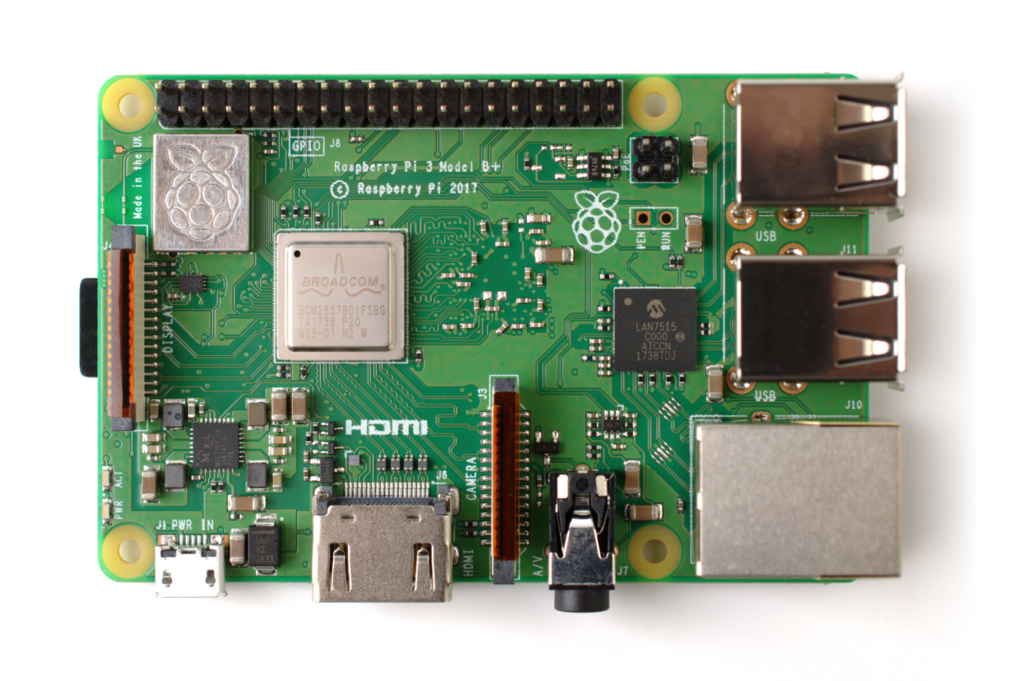
\includegraphics[scale = 0.3]{fig/Raspberry-Pi-3-modelo-B+.png}
\caption{Raspberry Pi 3 modelo B+}
\label{fig:raspberry-pi-3-modelo-Bplus}
\end{figure}

\subsubsection{Raspberry Pi 3 modelo A+}

\noindent Este modelo, que apareció en noviembre de 2018, no tenía por objeto mejorar las capacidades de sus predecesoras, si no presentar un precio más competitivo. Es por ello que, en este económico modelo contó con 512MB de RAM, un único puerto USB y eliminó la conexión RJ-45.

\subsubsection{Raspberry Pi 4 modelo B+}

\noindent Anunciada en junio de 2019, la Raspberry Pi 4 modelo B+ representa el prototipo más moderno durante la redacción de este trabajo de fin de grado. Este modelo cuenta con múltiples mejoras respecto a los modelos anteriores, entre las que pueden destacarse un procesador hasta 3 veces más eficiente que el anterior, la inclusión de una entrada USB 3.0 y el cambio de un puerto HDMI por dos puertos mini-HDMI. Este último modelo de Raspberry Pi se expone gráficamente en la figura~\ref{fig:raspberry-pi-4-modelo-B}.

\begin{figure}[tbp]
\centering
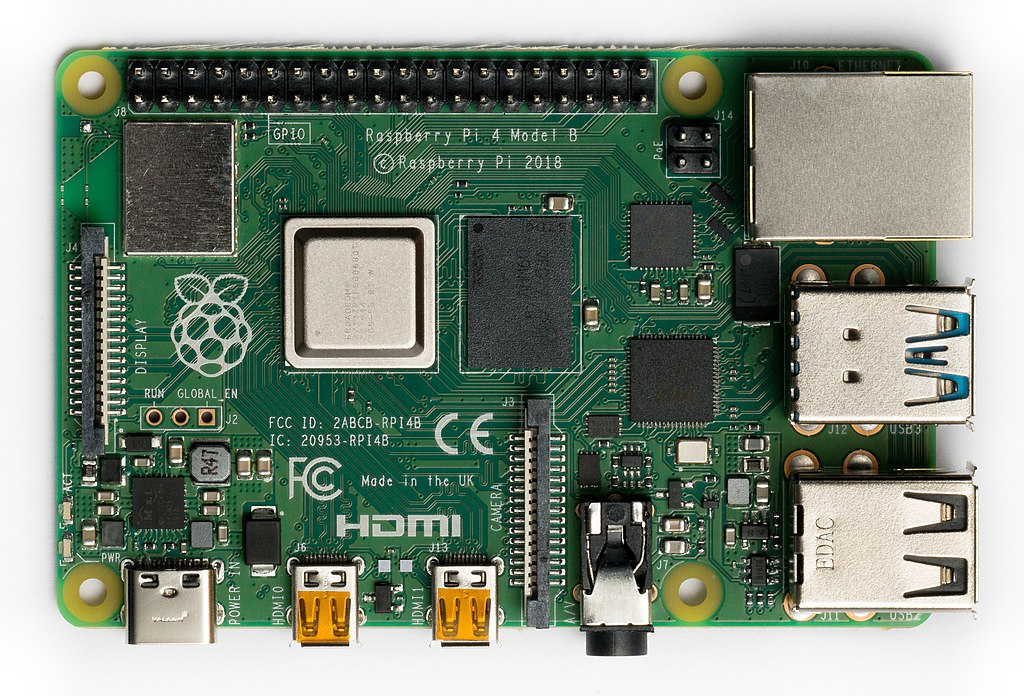
\includegraphics[scale = 0.3]{fig/Raspberry-Pi-4-modelo-B.jpg}
\caption{Raspberry Pi 4 modelo B}
\label{fig:raspberry-pi-4-modelo-B}
\end{figure}

Adicionalmente a los modelos básicos, la fundación Raspberry Pi también ha comercializado una gama de placas de menor coste y tamaño, llamadas Raspberry Pi Zero. Hasta la fecha, han aparecido tres modelos de este tipo de computadoras de bajo coste.

\subsubsection{Raspberry Pi Zero}

\noindent Hizo su aparición en 2015, y para entonces contaba ya con un procesador de 1GHz, 512MB de RAM. Debido a su diminuto tamaño, en lugar de usar los puertos HDMI y USB clásicos, hace uso de una entrada MiniHDMI y dos entradas MicroUSB. En la figura~\ref{fig:raspberry-pi-zero} se muestra esta mini computadora de bajo coste.

\begin{figure}[tbp]
\centering
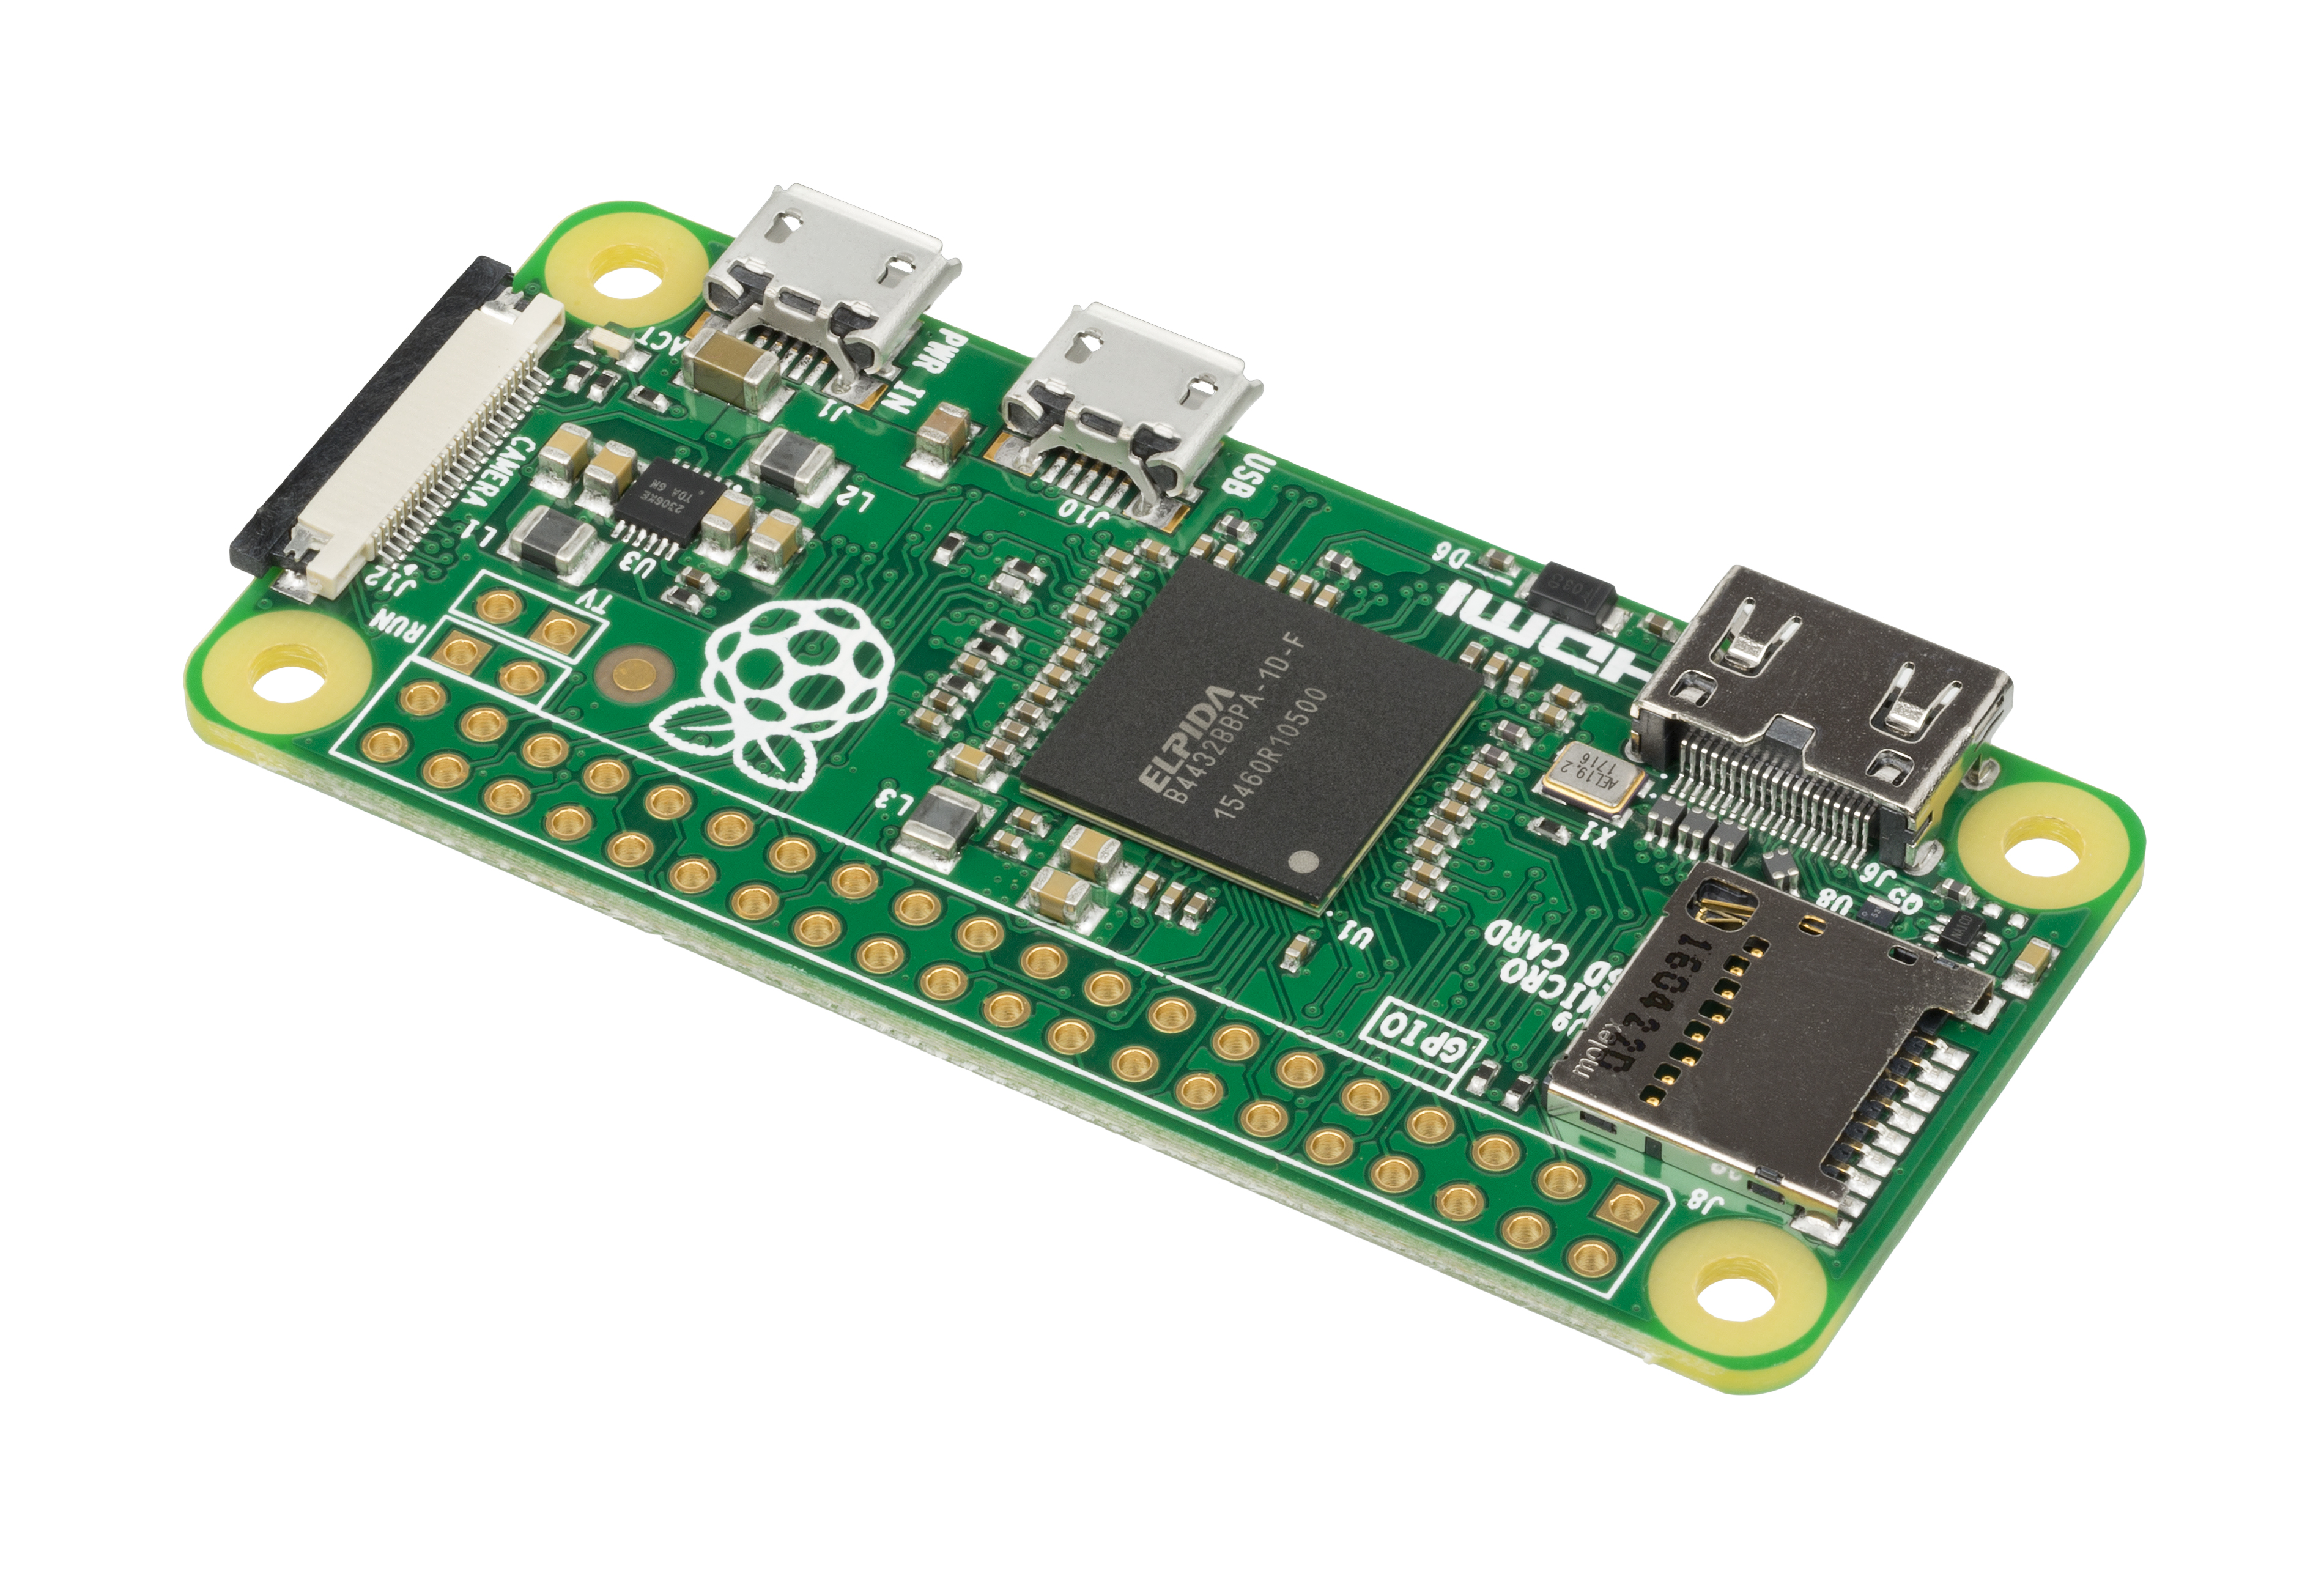
\includegraphics[scale = 0.24]{fig/Raspberry-Pi-Zero.jpg}
\caption{Raspberry Pi Zero}
\label{fig:raspberry-pi-zero}
\end{figure}

\subsubsection{Raspberry Pi Zero W}

\noindent La novedad que presenta este modelo respecto de su predecesora, es la inclusión de conexión por Bluetooth y Wi-Fi. Puede observarse este modelo de computadora en la figura~\ref{fig:raspberry-pi-zero-w}.

\begin{figure}[tbp]
\centering
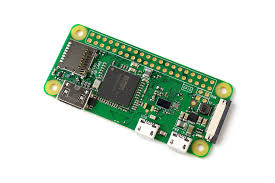
\includegraphics[scale = 1.2]{fig/Raspberry-Pi-Zero-W.jpg}
\caption{Raspberry Pi Zero W}
\label{fig:raspberry-pi-zero-w}
\end{figure}

\subsubsection{Raspberry Pi Zero WH}

\noindent Tan solo existe una diferencia entre este modelo y la Raspberry Pi  Zero W, y es la inclusión de un conector soldado a los 40 pines GPIO. Si quiere observarse la diferencia a nivel físico, no hay más que comparar esta computadora en la figura 1.7 con su predecesora en la figura~\ref{fig:raspberry-pi-zero-wh}.

\begin{figure}[tbp]
\centering
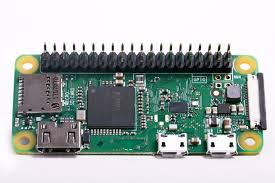
\includegraphics[scale = 0.8]{fig/Raspberry-Pi-Zero-WH.jpg}
\caption{Raspberry Pi Zero WH}
\label{fig:raspberry-pi-zero-wh}
\end{figure}

\subsection{Historia de los bots conversacionales}

\noindent En los tiempos que transcurren durante el desarrollo de este trabajo de fin de grado, los bots conversacionales parecen estar abriéndose camino a un público cada vez más amplío. Empresas como Microsoft, Google o Amazon apuestan por este tipo de tecnología, tratando de adaptarse a las necesidades de la gente con ayuda de algoritmos de inteligencia artificial.

Una buena forma de analizar la evolución de los bots, es por medio del test de Turing. En 1950, el matemático británico Alan Turing propuso un test a partir del cual se define la capacidad de un bot. La realización de dicho test consiste en ofrecer una serie de respuestas a un humano, que tendrá que decidir si estas han sido proporcionadas por otro humano o por una computadora.

Inspirado por el trabajo de Turing, el alemán Joseph Weizenbaum, desarrolló en 1966 el que sería el primer bot de la historia, al cual bautizó con el nombre de "ELIZA". Este bot consistía en un algoritmo que trataba de reconocer ciertas palabras clave, a partir de las cuales, ofrecía respuestas lógicas. Durante las pruebas conversacionales ejercidas entre humanos y ELIZA, múltiples personas creyeron estar hablando con un humano y compartieron con este bot detalles íntimos, haciendo de esta manera que ELIZA superara, a nivel teórico, el test de Turing.

De esta manera, en el 2000, apoyándose en la base establecida por sus predecesores, apareció SmarterChild, un bot capaz de procesar y entender de cierta manera el lenguaje, ofreciendo respuestas que permitían ayudar al usuario, con temas tan diversos como previsiones de meteorología o entradas de cine. SmarterChild era además compatible con plataformas de mensajería conocidas como MSN Messenger, y estableció por tanto un primer contacto entre el mundo de los bots conversacionales y el público general.

Desde entonces, la propagación de los bots, tanto de voz como escritos, se ha extendido en múltiples campos y plataformas. Desde los asistentes virtuales como Alexa y Google Home, hasta los múltiples bots de Telegram\cite{elenasantos2018} que permiten, entre otras muchas cosas, obtener imágenes de cualquier cosa con solo pedirlas o conocer la predicción meteorológica.

A finales del año 2018 ya se encontraban en funcionamiento\cite{albertoiglesiasfraga2019} más de 2.500 millones de asistentes virtuales, lo cual da muestra del estado de buena salud por el que pasa este tipo de tecnología.

\fi

\if00
\chapter{Procedimiento}
\label{ch:procedimiento}

En el desarrollo de este TFG se ha utilizado una metodología ágil basada en \emph{Scrum}~\cite{scrumguide}, definida por el director.  El trabajo se ha dividido en iteraciones de dos semanas denominadas \emph{sprints}.  Las unidades de trabajo se presentan en forma de historias de usuario (\emph{user stories}) que definen mini-proyectos de muy corta duración que aportan valor al proyecto.  Es decir, cada historia de usuario cumple o ayuda a cumplir alguno de los objetivos.  Medir el valor percibido corresponde al propietario del producto (\emph{Product Owner}), que participa activamente en la planificación del proceso priorizando las unidades de trabajo.

La utilización de una metodología ágil permite equilibrar la cantidad de trabajo y los objetivos alcanzados.  Los 12 créditos ECTS del TFG se reparten según el criterio del director para que los resultados aporten el máximo valor posible, incluso en presencia de imprevistos.

\section{Diferencias con Scrum}

\emph{Scrum} es una metodología estrictamente centrada en el cliente.  El cliente es el responsable de priorizar y, en cierto modo, planificar las iteraciones.  Esto garantiza que la ejecución del proyecto responde al máximo con las expectativas del cliente, aún cuando los imprevistos impidan alcanzar alguno de los objetivos iniciales.  Esta característica de \emph{Scrum} es la única que se ha intentado mantener inalterada.  Sin embargo, el TFG es un proyecto individual, lo que ha requerido modificar significativamente otros aspectos de la metodología.

\subsection{Roles}

La única remuneración que se obtiene con la ejecución de un TFG es la calificación de los distintos aspectos (anteproyecto, valoración del director, valoración del tribunal, etc.).  Por tanto, el cliente del TFG se compone por el director y el tribunal de la defensa.  Desgraciadamente no es posible conocer a priori el tribunal.  Por este motivo el director es el único representante del cliente en el proceso de desarrollo (\emph{Product Owner}).

El TFG debe ser realizado de manera individual.  Por tanto, el equipo de trabajo (\emph{Team Member}) se compone exclusivamente por el autor.

La labor de dirección del TFG se asimila a la de dirección del proyecto y, por tanto, el director también actúa como coordinador del proceso, o \emph{Scrum Master}.  Nótese que hay dos roles representados por la misma persona.  Desde un punto de vista purista esto implica que puede haber conflicto de intereses y los intereses del cliente pueden estar insuficientemente representados.  Es una limitación extrínseca, que no es posible solucionar con el proceso actual.  Aún así, el uso de una metodología ágil centrada en el cliente debe mejorar el alineamiento de intereses cuando sobrevienen problemas que afectan o pueden afectar a la consecución de alguno de los objetivos iniciales.

\subsection{Historias de usuario}

\emph{Scrum}, como la mayoría de los métodos ágiles, está enfocada al desarrollo de proyectos en entornos de alta incertidumbre por equipos multidisciplinares bien formados.  El desarrollo de un TFG, al tratarse de un primer proyecto profesional, también está sometido a gran cantidad de incertidumbre.  Sin embargo, no siempre se cuenta con la formación previa necesaria para abordar todos los problemas.  Esto implica que, en ocasiones, se necesita aprender o leer, sin repercusión medible en el valor percibido por el \emph{Product Owner}.  En esos casos se planifican unidades de trabajo que no corresponden estrictamente a historias de usuario en el sentido de Scrum.  Se ha intentado mantener al mínimo este tipo de historias de usuario para tener el proceso lo más controlado posible.

Puntualmente ha sido necesario planificar historias de usuario que solo pretenden explorar opciones.  Este tipo de historias de usuario están contempladas en \emph{Scrum}, se denominan \emph{spikes}.  Sin embargo, en la ejecución de este TFG se ha procurado reducir al mínimo para que la exploración de alternativas no domine en el tiempo dedicado al TFG.

\subsection{Planificación de sprints}

Para la planificación y el seguimiento se ha utilizado un tablero \href{http://trello.com}{Trello}.  Los tableros Trello permiten agrupar tarjetas en una serie de listas con nombre.  Se ha utilizado el esquema propuesto en~\cite{andrewlittlefield2018}.

El autor ha sido responsable de añadir la mayoría de las historias de usuario a la lista \emph{Backlog}.  Se trata de un proceso continuo, durante toda la ejecución del proyecto.  El director, como \emph{product owner}, prioriza las historias, moviendo las tarjetas dentro de la lista \emph{Backlog}.  Justo antes de cada iteración se realiza una reunión presencial o virtual para revisar la iteración pasada y planificar la siguiente iteración.

Usando la técnica de \emph{planning poker} (ver~\cite{scrumguide}) se dimensionan las historias de usuario en días de trabajo.  Esta técnica consiste en un proceso de generación de consenso entre el autor y el director sobre el tiempo requerido para la ejecución de cada historia de usuario.  La unidad empleada ha sido de un día.

El director, como \emph{product owner} traslada las tarjetas correspondientes a las primeras historias de la lista \emph{Backlog} a la lista \emph{ToDo} hasta completar los 10 días de trabajo de la iteración.

\subsection{Flujo de trabajo}

El flujo de trabajo diario del autor corresponde a la siguiente secuencia:

\begin{itemize}
    \item Dentro de la lista \emph{ToDo} puede elegirse cualquier tarjeta para trabajar en ella.  Antes de comenzar el trabajo se arrastra la tarjeta a la lista \emph{Doing}.  Esto proporciona información en tiempo real al director del progreso de la iteración.
    
    \item Al terminar una historia de usuario la tarjeta correspondiente se arrastra a la lista \emph{QC} (quality control).
    
    \item El director, como \emph{Scrum Master}, revisa que la historia está realmente acabada y, si así es, la traslada a la lista \emph{Done}. En caso contrario la traslada a la lista \emph{Doing} otra vez, añadiendo un comentario que lo justifica.

    \item Si en el transcurso del trabajo se encuentra un obstáculo que impide progresar con una historia, se traslada a la lista \emph{Blocked}, añadiendo un comentario que lo justifica.
\end{itemize}

En todo momento es posible ver el estado global de ejecución del proyecto.  Al finalizar, la lista \emph{Done} contiene todas las historias de usuario ejecutadas por orden de terminación.  Y las listas \emph{Blocked} y \emph{Backlog} contienen (en este orden) todas las historias de usuario que corresponderían a trabajo futuro, ya priorizadas por el director.

\subsection{Herramientas de ayuda}

El proceso de desarrollo está fuertemente ligado a la herramienta \href{https://trello.com/}{Trello}.  Se trata de una herramienta colaborativa en línea, que permite mantener una serie de tarjetas agrupadas en listas con nombre.  Cada tarjeta puede tener un título, una descripción, un conjunto de adjuntos, y un conjunto de comentarios.  Trello se ha usado con éxito en la planificación de proyectos de nivel de complejidad muy variable.  Por ejemplo, Epic Games utiliza un tablero Trello para planificar las características a incorporar a cada nueva versión de Unreal Engine.  Por otro lado, un problema de Trello es el manejo limitado de la historia de modificaciones en las tarjetas y en los movimientos entre listas de tarjetas.  Esto dificulta en cierto modo el seguimiento de los cambios y, sobre todo, la corrección de errores en el proceso.  Por este motivo, Trello solo se ha empleado en la coordinación del trabajo, mientras que toda la gestión de cambios se ha delegado en otra herramienta.

Todo el proyecto ha sido gestionado desde su inicio con una herramienta de control de versiones distribuido en un repositorio público de GitHub, disponible en \thegitrepo.  Cada vez que se completa con éxito una historia de usuario se notifica mediante un comentario en la tarjeta correspondiente.  Este comentario tan solo contiene el identificador del paquete de cambios (\emph{commit}) que da por concluida la historia.  Todos los \emph{stakeholders} pueden consultar la evolución del proyecto en todo momento desde la propia página del repositorio.

\begin{figure}[tbp]
\centering
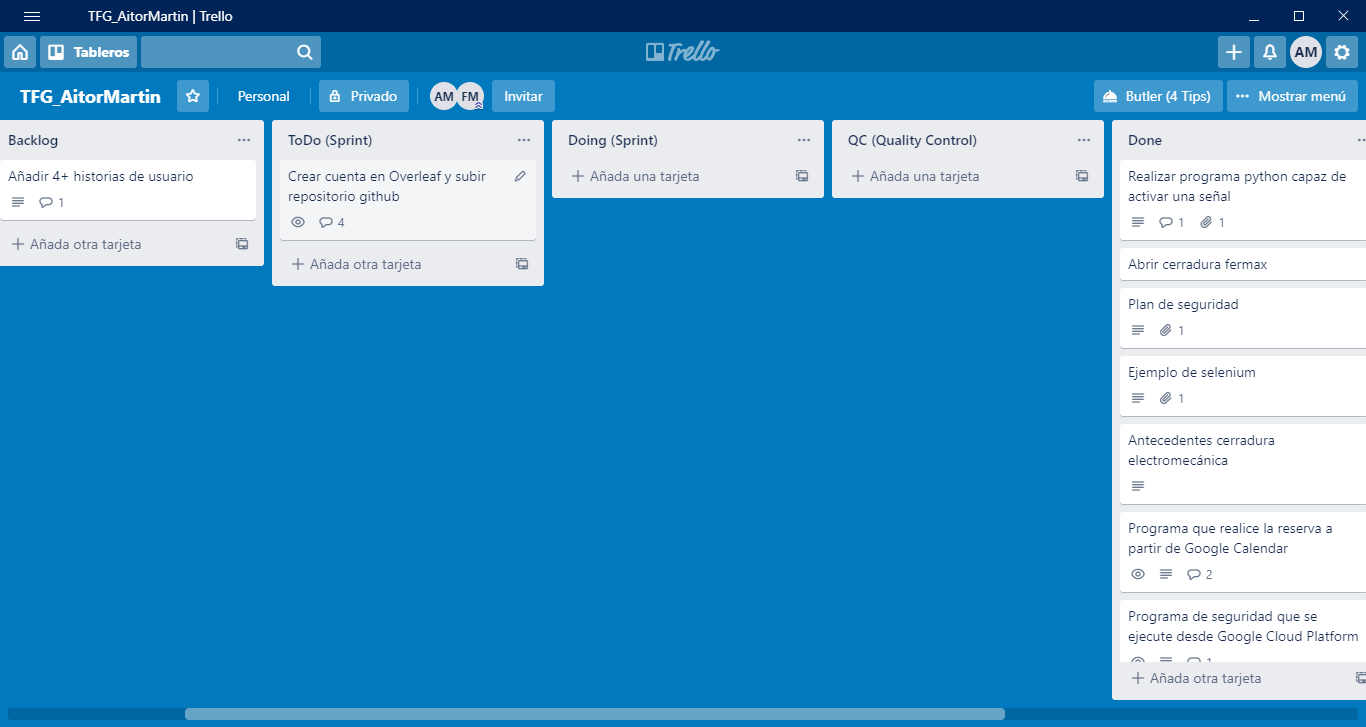
\includegraphics[scale = 0.4]{fig/tableto-trello.PNG}
\caption{Tableto trello utilizado en el desarrollo de este trabajo de fin de grado}
\label{fig:tableto-de-trello}
\end{figure}
\fi

\if00
\chapter{Desarrollo del TFG}
\label{ch:desarrollo}

\section{Metodología empleada: Scrum} 
\label{sec:metodologia-empleada}

Durante el desarrollo de este trabajo de fin de grado se ha hecho uso de una metodología Scrum \cite{andrewlittlefield2018}. Sin embargo, este sistema no se ha aplicado de forma estricta, si no que se han modificado algunos aspectos, adaptándolo a las necesidades que este trabajo de fin de grado ha requerido, tal como puede observarse en las siguientes líneas. 

\textbf{\large Backlog}
Este modelo comienza con un Product Owner, que es la persona que define cual será el resultado final esperado. En este caso, esta figura es personificada por el tutor de este TFG, Francisco Moya. Esta persona es también la encargada de definir el Backlog, que es la lista de tareas que serán necesarias para la realización completa del proyecto. En este caso, el Backlog ha sido elaborado por el tutor y el alumno.
Resulta de vital importancia que en el Backlog destaquen las prioridades, de manera que se resalte la importancia de aquellas tareas que implican una mayor responsabilidad a la hora de tener el producto final esperado.

\textbf{\large Sprint}
De forma posterior al Backlog, vendría el Sprint. En esta etapa se materializan los objetivos definidos previamente en el apartado Backlog. Cada etapa de Sprint debe finalizar con una revisión en la que los miembros del equipo discutan las formas de mejorar el proceso de ejecución. En nuestro TFG, la etapa de Sprint se ha dividido en dos partes principales:
\begin{enumerate}
\item \underline{ToDo.} Esta parte recoge todas las tareas extraídas del Backlog, que están por hacer. Es un punto decisivo para determinar la prioridad de cada una de las actividades, ya que aquellas que resulten de mayor interés serán transportadas al siguiente punto, donde se ejecutarán.
\item \underline{Doing.} Las tareas que se encuentran en este punto se encuentran en proceso de materialización. El apartado Doing implica el ecuador de este modelo de trabajo, ya que es el instante en el que se llevan a efecto los trabajos, que en conjunto, determinarán el resultado final del proyecto.
\end{enumerate}

\textbf{\large Quality Control}
Una vez que las tareas han sido realizadas en el apartado de Sprint, se procede a transportarlas hacia el Quality Control, o control de calidad, donde se hará un análisis sistemático de las mismas, en el que se determinará si estas han cumplido o no con los criterios exigidos. Durante el transcurso de este trabajo de fin de grado, el tutor Francisco Moya, ha sido quien ha trabajado este apartado aceptando, rechazando o proponiendo modificaciones siempre que lo ha considerado necesario. Del resultado de estas valoraciones se determinará si la tarea ha sido completada correctamente, o si por el contrario, necesita ser editada o replanteada.

\textbf{\large Done}
Una tarea acaba en el apartado Done cuando esta ha sido aceptada en su proceso de control de calidad. Que una tarea ocupe esta posición significa que no necesita más ediciones ni tampoco más revisiones, por lo que puede considerarse que se encuentra completamente terminada.

\textbf{\large Blocked}
El apartado Blocked comprende uno de los aspectos más importantes de la metodología Scrum. Cuando una tarea no puede ser completada, por cualquier circunstancia, se puede transportar a este apartado, donde un miembro o un equipo de jerarquía superior podrá determinar una solución. En el caso de este trabajo de fin de grado, el tutor Francisco Moya ha sido quien ha ido determinando las soluciones que se debían proponer a los problemas que el alumno ha ido transportando a esta posición.
\section{Planificación del proyecto} 
\label{sec:planificacion-del-proyecto}
Una vez definidos debidamente los objetivos y la metodología de trabajo, se procede a determinar cuál será la planificación del proyecto. Esta planificación implica la división que se ha realizado sobre el problema que se aborda, en todas las fases necesarias para la obtención de una solución satisfactoria y definitiva.

Este problema se afronta desde la división de 3 fases principales: circuito electrónico, diseño de algoritmos y programación, y por último, seguridad. Cada una de estas fases guarda dependencias entre sí, por lo que su ejecución no puede ser completamente independiente ni ir en un marco temporal diferente. La seguridad, por ejemplo, contempla uno de los aspectos más importantes a tener en cuenta en el proyecto, y aunque los trabajos de programación referidos a este apartado y las revisiones y modificaciones han venido al final del proyecto, todos los trabajos realizados anteriormente, en cualquiera de las fases, han tenido en cuenta este y otros factores. A continuación se definen, a través de las 3 fases principales, las tareas que se han propuesto durante el desarrollo de este trabajo de fin de grado.
\subsection{Construcción del circuito electrónico} 
El modelo de portero automático con el que se ha trabajado en este proyecto, es el FERMAX 8044, cuyas características técnicas se especificarán más adelante. Teniendo esto en cuenta, los trabajos orientados al desarrollo del circuito electrónico han debido adaptarse al funcionamiento de este modelo.

La primera parte del trabajo ha consistido, por tanto, en tratar de activar la apertura de una cerradura eléctrica, por medio de un portero automático, activado con una señal emitida por una Raspberry Pi Zero W. Para la consecución de esta tarea se han programado tareas de distinto ámbito, como son las siguientes:
\begin{enumerate}
\item \underline{Documentación de los elementos a emplear:} En primer lugar, con el fin de adquirir la información necesaria para llevar a cabo la ejecución correcta del circuito electrónico, se ha elaborado una tarea consistente en estudiar el funcionamiento de cada uno de los componentes que serán precisos.
\item \underline{Conexiones físicas:} Estas tarea consiste en determinar que elementos serán necesarios para el correcto funcionamiento del circuito, y una vez que este haya sido construido, en realizar la conexión de estos elementos.
\item \underline{Fijación de los elementos} Para que el transporte físico del prototipo sea seguro, se ha decidido incluir una tarea en este apartado con la que se garantice una sujeción firme.
\end{enumerate}
\subsection{Diseño de algoritmos y programación}
Sin duda, el grueso de este trabajo de fin de grado corresponde a la realización de todos los programas que permitirán el correcto cumplimiento de los objetivos definidos.
Esta tarea se ha dividido a su vez en diferentes subtareas, las cuales se definen a continuación:
\begin{enumerate}

\item \underline{Programa capaz de activar la señal:} A partir de la aplicación de mensajería instantánea "Telegram", esta tarea refiere la misión de conseguir que, a partir de una petición hecha por un usuario desde esta aplicación, se active una señal que, con el circuito elaborado previamente, active la señal que permita realizar la apertura de la puerta.
Este programa deberá incluir también un panel de administrador, con el fin de que el anfitrión tenga la posibilidad de crear accesos a la vivienda a aquellos usuarios que considere conveniente, así como cancelar estos accesos. Desde este panel, también se deberán incluir opciones de modificación de reservas y realizar las peticiones de acceso a la vivienda.
\item \underline{Programa capaz de recibir las reservas:} Esta tarea se considerará completada en el momento en que, al producirse una reserva en la plataforma de alquiler (en este proyecto se ha elegido Booking.com por ser la plataforma más utilizada en el mundo), el programa incluya la información de entrada en el sistema, y permita acceder al huésped, en la fecha definida y con su número de reserva, a la propiedad que ha alquilado.
\item \underline{Programa capaz de cancelar las reservas:} Al igual que se producen nuevas reservas, se producen cancelaciones, por lo que un sistema necesitará tenerlas en cuenta para funcionar de forma correcta. Es por ello que, en esta tarea se establece el desarrollo de un algoritmo que integre la información necesaria en el sistema al producirse una cancelación.
\item \underline{Unificar los programas anteriores:}Una vez que se cuente con los programas mencionados en los puntos anteriores, es de vital importancia hacer que funcionen de forma síncrona, por lo que el objetivo de esta tarea es el de cumplir con dicha exigencia.
\end{enumerate}
\subsection{Tareas orientadas a la seguridad del dispositivo}
Si se busca la definición de "seguro" en la Real Academia Española, podrá observarse que se define como "libre y exento de todo riesgo", y si se baja unas cuantas líneas más, encontraremos la siguiente definición: "que no falla o que ofrece confianza".
Garantizar, a día de hoy, un sistema conectado a la red que sea completamente seguro es algo prácticamente imposible para cualquier empresa. Algunas de ellas \cite{redaccionapd2018} como Yahoo, Telefónica o incluso el propio Pentágono, han sido protagonistas en más de una ocasión de haber caído en manos de ciberdelincuentes que, aprovechando cualquier vulnerabilidad, han conseguido introducirse en sus sistemas. Es por ello que, en este trabajo de fin de grado, se va a tratar de cumplir la segunda definición expuesta de "seguro", y no la primera.

Para que el sistema propuesto obtenga la confianza de los huéspedes, deberá conseguirla primero de los anfitriones, ya que son ellos quienes decidirán si este proyecto saldrá adelante. Para ello es necesario exponer, de forma clara, que se ha pensado en las diferentes posibilidades que podrían afectar el correcto funcionamiento de este sistema. 

Para evitar estas problemas de seguridad, se han definido tres tareas que deberán cumplirse antes:
\begin{enumerate}
\item \underline{Programa para prevenir manipulaciones malintencionadas:} Esta tarea se realiza con el fin de evitar que usuarios, de forma malintencionada, puedan manipular el correcto funcionamiento del sistema. Para ello, se establece la elaboración de un programa con el que se detecte, y se avise al anfitrión, de cualquier intento de acceder a la Raspberry Pi. Como la placa irá cerrada en una caja, esta tarea se considerará completada en el momento en que se pueda detectar si alguien ha abierto dicha caja, y en ese caso, avise al propietario, con el fin de que este pueda actuar de la forma que considere oportuna.
\item \underline{Programa que avise en caso de interrupción del funcionamiento: } De nada serviría la tarea descrita en el punto anterior si no se tiene en cuenta la posibilidad de una interrupción del funcionamiento. En caso de que un usuario malintencionado cortara la corriente o el acceso a internet antes de abrir la caja, no habría a quién avisar. Es por ello que se pretende ir más allá en este punto, incluyendo una tarea con la que se detecte cualquier interrupción del correcto funcionamiento de nuestra Raspberry Pi por medio de su monitorización y sistema automático de aviso. De esta manera, el anfitrión tendrá la tranquilidad de que todo funciona de forma correcta, y en caso de que algo falle, sabrá que será avisado y podrá tener todo en orden.
\item \underline{Seguridad a nivel físico:} Una de las mejores formas de garantizar la seguridad, es impidiendo la consecución de actos indeseados de forma física. Para que este objeto llegue a buen puerto, se exigirá por medio de esta tarea la realización de un diseño en tres dimensiones de la caja que contendrá el prototipo. Este diseño deberá cumplir varios criterios:
\begin{itemize}
\item{Ofrecer la posibilidad de un cerramiento anclado por medio de un candado.}
\item{Contar con las características físicas necesarias para poder anclar de forma correcta los elementos que conforman el prototipo.}
\end{itemize}
\item \underline{Adaptación del programa inicial de seguridad al prototipo:} Una vez que se tenga el prototipo, se deberán realizar las comprobaciones y modificaciones pertinentes en el programa que se creó para evitar manipulaciones malintencionadas, de manera que se adapte a las medidas y parámetros que resulten de conveniencia con el fin de garantizar la seguridad y el correcto funcionamiento de todo el sistema.
\end{enumerate}

\section{Ejecución del proyecto} 
\label{sec:ejecucion-del-proyecto}
Con la metodología clara y la planificación debidamente definida, se procede a realizar la ejecución material del proyecto. El orden que seguirá este apartado será idéntico al de las tareas. En cada punto se explicarán las operaciones realizadas y los problemas o limitaciones que se han encontrado en cada una de ellas.

A continuación se procede a definir la ejecución de las actividades desarrolladas durante el transcurso de este trabajo de fin de grado.

\subsection{Construcción del circuito electrónico:}
La función principal que debe desarrollar el circuito electrónico, objeto de este apartado, es la de realizar la apertura de una cerradura eléctrica a partir de una señal emitida por la Raspberry Pi. Para llevar a cabo tal objetivo, es necesario hacer uso de un portero automático, ya que en todas las viviendas nos encontramos que es este aparato el que trabaja de forma directa con la cerradura.
Por tanto, la construcción de este prototipo debe comenzar por la conexión entre estos dos elementos, lo cual obliga a recoger la documentación técnica necesaria de ambos elementos. Para ello, se debe buscar la hoja de datos correspondiente al portero automático FERMAX 8044\footnote{\url{https://www.fermax.com/spain/pro/documentacion/documentacion-tecnica/DT-10-manuales.html?searchword=8044&subfamily=}}, y a la cerradura DORCAS modelo 41\footnote{\url{https://www.dorcas.com/wp-content/uploads/2016/01/Catalogo_General_Dorcas.pdf}}.

Analizando las hojas de características de estos dos elementos, se comprueba que la cerradura eléctrica permite su activación con señales de 12V en alterna, tensión compatible con el funcionamiento del portero automático elegido.
Para un desarrollo correcto, hay que remarcar que el portero no solo debe funcionar para el propósito de este prototipo, si no que debe permitir el correcto funcionamiento de su actividad habitual de realizar aperturas por medio de los usuarios de la vivienda. Es por ello que la instalación del portero debe ser la habitual, y una vez que se tenga instalado, es el prototipo el que debe adaptarse al funcionamiento del mismo.

Para realizar el esquema de instalación se hace uso de los siguientes elementos:
\begin{itemize}
\item{Portero automático | Modelo FERMAX 8044}
\item{Transformador | Modelo DORCAS 30078}
\item{Cerradura eléctrica | Modelo DORCAS 41}
\end{itemize}
El esquema de la instalación del portero automático, para realizar aperturas con la cerradura eléctrica, sería tal como puede observarse en la figura~\ref{fig:conexion-portero-cerradura}.
\begin{figure}[tbp]
\centering
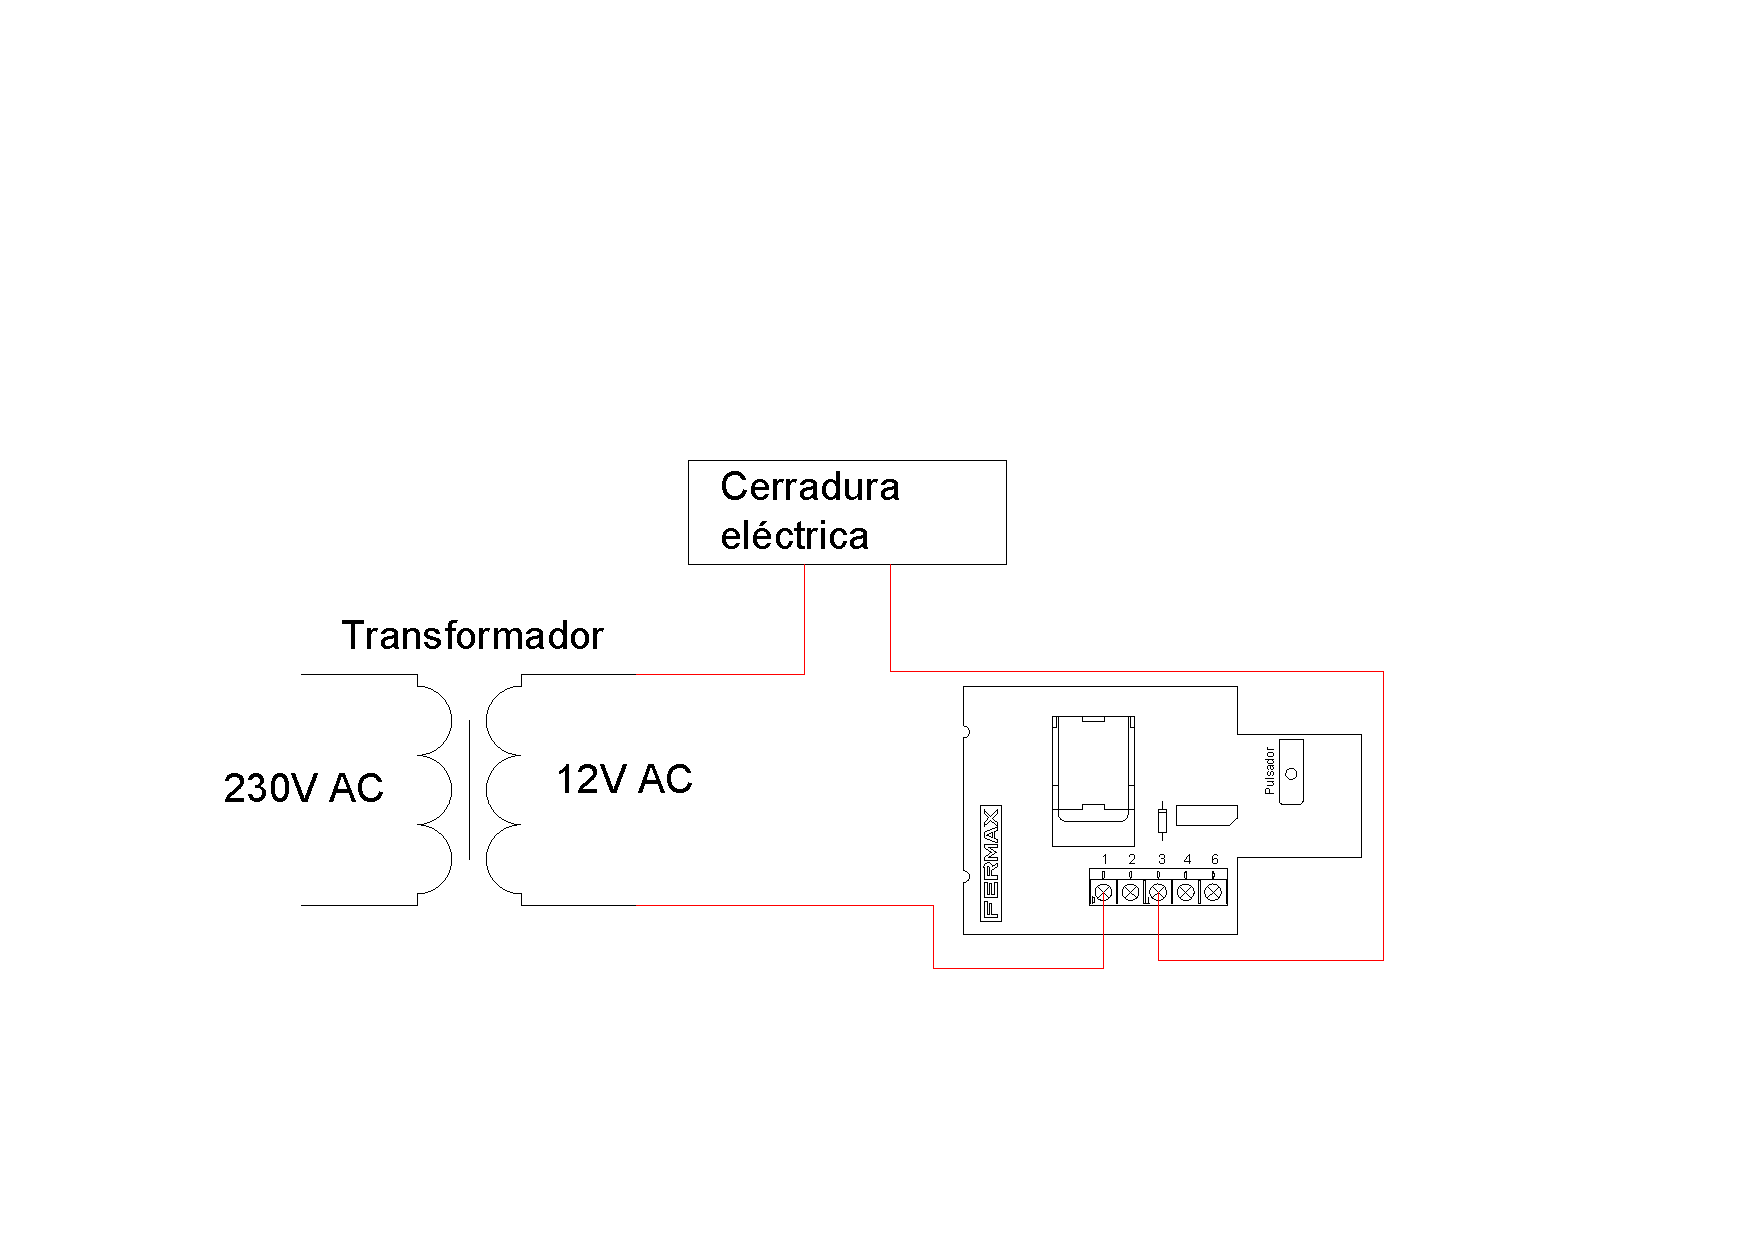
\includegraphics[scale = 0.5]{Conexion-Portero-Cerradura.pdf}
\caption{Conexión de funcionamiento entre el portero automático y la cerradura eléctrica}
\label{fig:conexion-portero-cerradura}
\end{figure}
Como puede observarse en la figura~\ref{fig:conexion-portero-cerradura}, la cerradura eléctrica se activaría siempre que el portero automático permita el paso de corriente. En el caso habitual, el accionamiento del pulsador por parte de cualquier usuario permitiría esta conducción de corriente, sin embargo, en el caso de este trabajo de fin de grado, se debe lograr tal propósito por medio de la activación de una señal de 3V, que es la que la Raspberry Pi Zero W permite emitir a partir de sus puertos programables.

Para llevar a efecto esta tarea será necesario realizar un circuito adicional que permita, siempre que se considere oportuno, el paso de corriente entre los dos bornes del pulsador, haciendo así que el circuito se cierre y se abra cuando se accione la señal emitida por la Raspberry Pi.

Con el fin de resolver este problema, se ha hecho uso de los siguientes elementos:
\begin{itemize}
\item{Relé 5VDC | Modelo: TONGLING JQC-3FF-S-Z}
\item{Conversor de niveles lógicos 3.3/5V | Modelo: Qifei cyt1082}
\item{Raspberry Pi Zero W}
\end{itemize}
En la figura~\ref{fig:conexion-keyhome-completa} se describe el circuito completo que permite realizar la apertura de la cerradura eléctrica por medio de una señal de 3.3V emitida por una Raspberry Pi Zero W:
\begin{figure}[tbp]
\centering
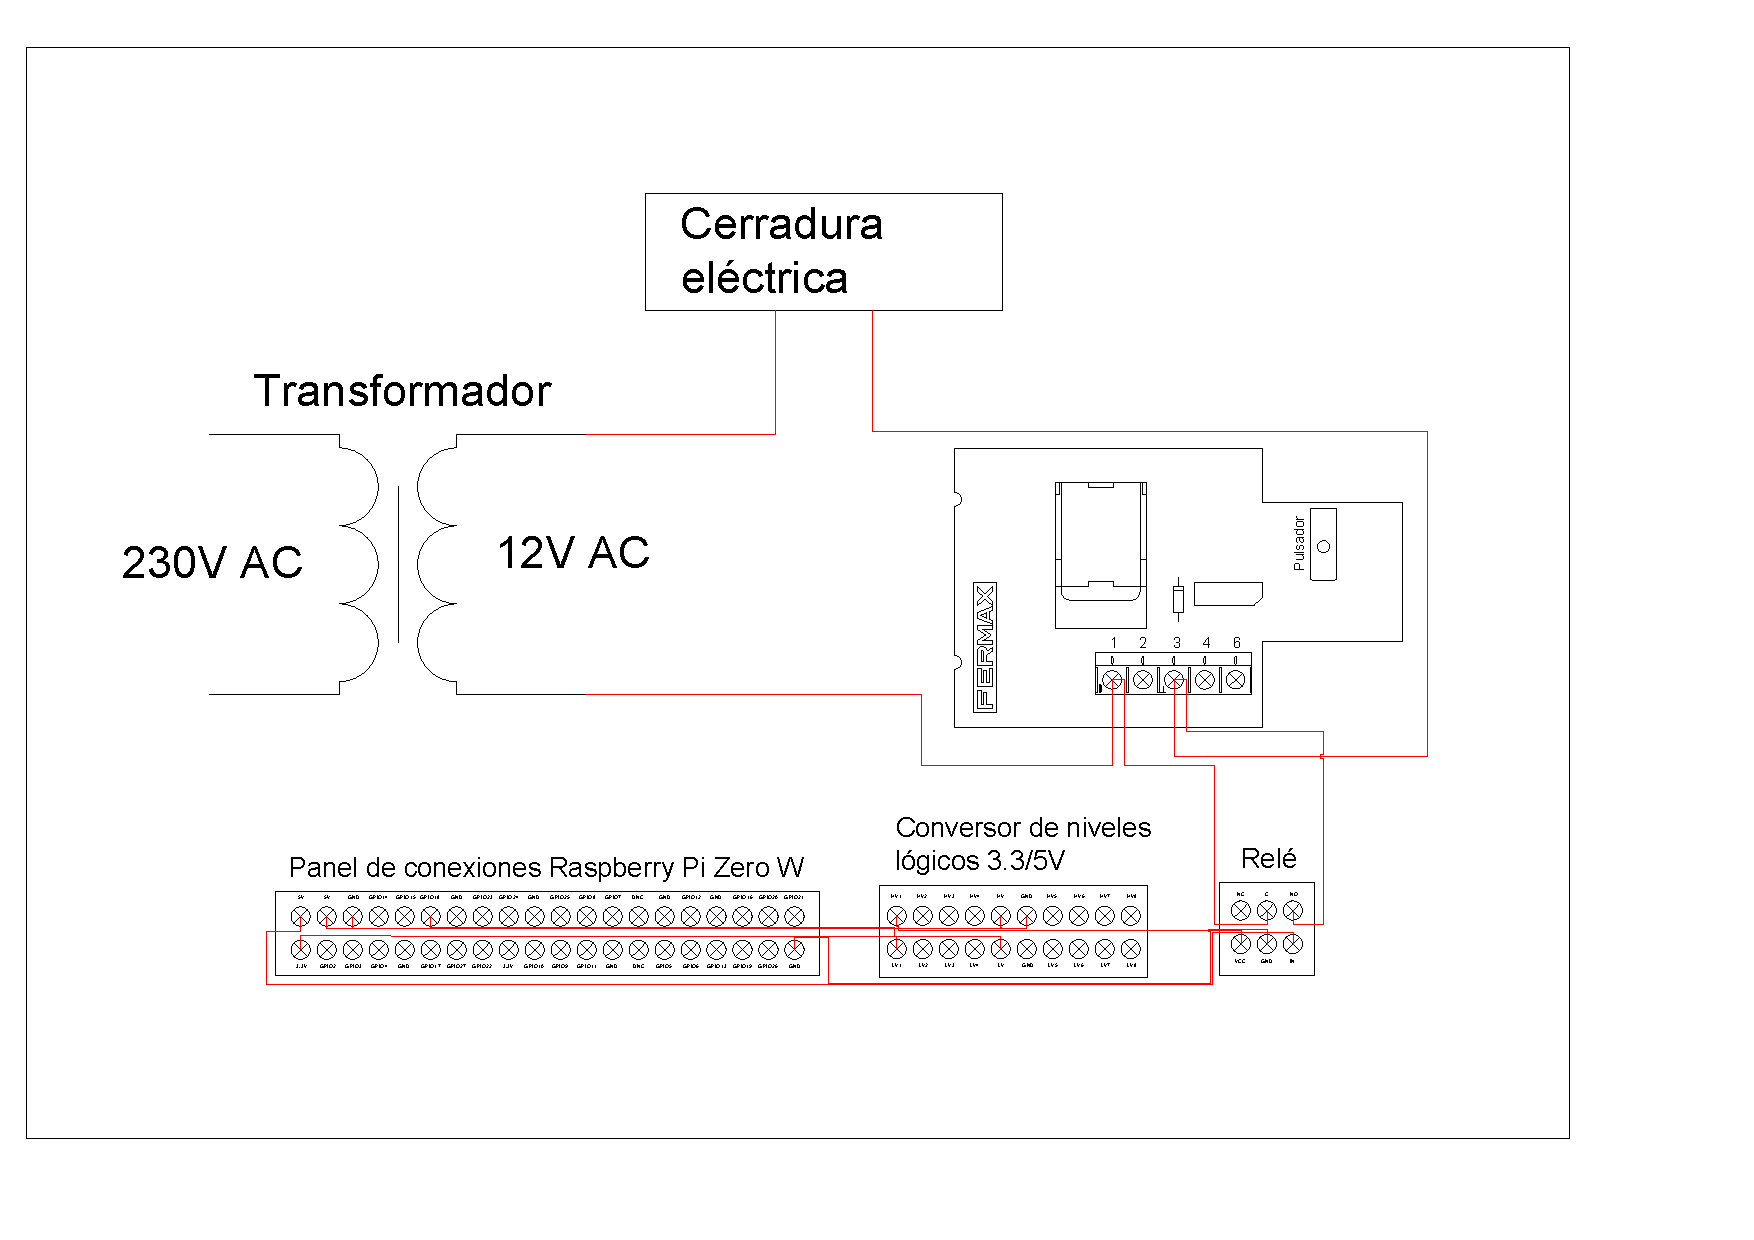
\includegraphics[scale = 0.5]{conexion-keyhome-completa.pdf}
\caption{Conexión de funcionamiento del prototipo completo}
\label{fig:conexion-keyhome-completa}
\end{figure}
Ahora, con el nuevo planteamiento especificado en este circuito, se obtiene el resultado esperado, haciendo que además de poder realizar la apertura de la cerradura por medio de una pulsación física sobre el pulsador del portero automático, pueda hacerse a través de una señal emitida por la Raspberry Pi Zero W con valor de 3V.
Para que se active dicha cerradura eléctrica es necesario que el circuito se cierre sin necesidad de hacer uso del pulsador, y para ello se ha hecho uso de un relé que, al recibir una señal de 5V, permite el paso de corriente entre los terminales 1 y 3 del portero automático.

Como las señales emitidas por la Raspberry Pi son de 5V, no sirven para realizar la activación del señal, por ello se ha empleado un conversor de niveles lógicos que convierte dicha señal de 3V en una de 5V, haciendo así que la señal recibida por el relé permita, de forma correcta, el paso de corriente entre sus terminales.
Con este nuevo diseño, la corriente encuentra dos lugares a través de los cuales puede circular, según se requiera:
\begin{itemize}
\item{A través de los terminales del pulsador cuando este es activado}
\item{A través del relé cuando este recibe una señal de la Raspberry Pi Zero W}
\end{itemize}
Con el fin de poder transportar el prototipo de forma segura y de que las conexiones sean estables, se ha procedido a soldarlas y a fijar cada uno de los elementos con firmeza en una tabla.

\subsection{Diseño de algoritmos y programación}
Una vez que el prototipo ha sido desarrollado y probado con éxito, llega el momento de hacer que las señales se activen en el momento correcto, de manera que todo funcione de forma precisa. Para ello, tal como se ha definido en el apartado de planificación del proyecto, se ha decidido dividir el desarrollo de software en cuatro etapas diferenciadas que, una vez completadas, harán que el prototipo proporcione los resultados esperados. En este apartado se describen los trabajos desarrollados en el orden lógico temporal que fueron realizados.

Lo primero que debe tenerse en cuenta es que la versión de python que viene por defecto en este modelo de Raspberry Pi, es la 2, mientras que la librería ApiTelegramBotAPI, encargada de ejecutar las funciones del bot, funciona con python3, por lo que será necesario instalar esta versión de python\footnote{\url{https://www.altaruru.com/python3-6-en-raspberry-pi/}} en la computadora, de forma previa a la ejecución de los programas previstos.

Antes de llevar a cabo la elaboración de ningún programa, es preciso realizar las configuraciones que permitan trabajar en la Raspberry Pi Zero W con las librerías que se ejecutarán en los archivos de python, de manera que todo funcione y se ejecute de forma correcta. Para llevar a cabo, se hace uso del sistema de gestión de paquetes llamado "pip", el cual permite la instalación de las distintas librerías, necesarias para la ejecución material de este proyecto, de forma sencilla. Para hacer uso de este sistema en la instalación de paquetes para python3, simplemente debe ejecutarse el comando "sudo pip3 install --upgrade pip" en la consola de la Raspberry Pi, y de esta manera se dispondrá de la última versión de este instalador.

Cuando se cuenta con "pip3", la instalación de los paquetes se resume a una ecuación de carácter sencilla, que se ejecutará en la consola de comandos y seguirá siempre la siguiente estructura:

\begin{equation} 
pip3 + install + "Nombre_paquete"
\label{eq:funcionamiento-pip3}
\end{equation}

El primer programa que se pretende definir es aquel que hará que la Raspberry Pi Zero W envíe una señal con el fin de activar la cerradura eléctrica en los momentos que resulten convenientes. A lo largo de este subcapítulo, se irán mostrando y comentando las distintas partes del código que permite cumplir dichas funciones.

\begin{lstlisting}[language=Python,
    caption={Importación de librerias},
    label=src:importacion-librerias
]
import RPi.GPIO as GPIO
import time
GPIO.setmode(GPIO.BCM)
GPIO.setup(18, GPIO.OUT)
import telebot
from telebot import types
import unidecode
import random
from datetime import datetime, date, timedelta
import calendar
\end{lstlisting}

Lo primero que se realiza en el código, tal como puede observarse en el listado 5.1, es importar cada una de las librerías que serán necesarias para su desarrollo. Estas librerías están destinadas a trabajos diversos, como puede ser implementar la funcionalidad del envío de señales por medio de la Raspberry Pi, trabajar con la aplicación de Telegram, hacer uso de números aleatorios u operar con fechas. Todas estas librerías desarrollarán funciones específicas a lo largo del código que puede observarse en el listado 5.2.
\begin{lstlisting}[language=Python,
    caption={Inicializar variables},
    label=src:inicializar-variables
]
fechasiniciales=[]
fechasfinales=[]
contrasenas=[]
fechainiciousuario=[]
fechafinalusuario=[]
fechas = str(datetime.now())
ano = int(fechas[0:4])
mes = int(fechas[5:7])
dia = int(fechas[8:10])
usuariosactivos=[]
administradores=[]
listanegra=[]
paso1=False
paso2=False
paso3=False
paso0=False
intentos = 0 
contador_intentos_erroneos = []
numreserva = ""
bot = telebot.TeleBot('TOKEN')
\end{lstlisting}
En el listado 5.2 se procede a inicializar algunas de las variables con las que se irán trabajando a lo largo de este programa. También se incluye en esta parte el Token ofrecido por la plataforma de Telegram, el cual permite conectar con el bot de forma segura.
\begin{lstlisting}[language=Python,
    caption={Función que convierte el string de reservas en un vector},
    label=src:string-a-vector
]
def convierteavector(texto):
    if len(texto) > 0:
        texto = texto.replace("'","")
        texto = texto.replace("[","")
        texto = texto.replace("]","")
        texto = texto.replace(" ","")
        vector = texto.split(',')
        return vector
\end{lstlisting}
La función que se muestra en el listado 5.4 servirá para convertir una cadena de texto común en un vector, que como se verá más adelante, resultará de utilidad para el correcto funcionamiento del programa. Las reservas que se irán recibiendo, tanto las creadas por parte del administrador como las que se reciban de las compañías de alquiler vacacional, se irán almacenando en un documento de extensión .txt que registrará el número de reserva y la fecha de entrada. Estos datos estarán almacenados en un vector que será convertido a texto con el fin de integrarse en el documento .txt de forma que, aunque la Raspberry Pi Zero W se apague, la información se pueda recuperar de forma segura.
\begin{lstlisting}[language=Python,
    caption={Función que verifica si una petición es posterior a la fecha inicial de la reserva},
    label=src:comprueba-fecha-inicial
]
def comprobarfecha(fechainic):
    fechas = str(datetime.now())
    ano = int(fechas[0:4])
    mes = int(fechas[5:7])
    dia = int(fechas[8:10])
    hora = int(fechas[11:13])
    anop = int(fechainic[0:4])
    mesp = int(fechainic[5:7])
    diap = int(fechainic[8:10])
    if anop == ano and mesp == mes and diap == dia:
        if hora >= 15:
            return True
        else:
            return False   
    elif ano > anop:
        return True
    elif ano == anop and mes > mesp:
        return True
    elif ano == anop and mes == mesp and dia >= diap:
        return True
    else:
        return False
\end{lstlisting}
En el listado 5.4 se muestra una función que servirá al programa para verificar si la persona que trata de acceder a la vivienda lo hace en un marco temporal posterior a la fecha inicial de su reserva. En caso de que se cumpla, devolverá un booleano verdadero y, en caso de que no se cumpla, devolverá un booleano falso. Puede observarse que la hora mínima que se ha puesto para acceder a la vivienda son las 15pm. Esta decisión se ha tomado ya que parece ser el horario habitual en la mayoría de destinos hoteleros, sin embargo este es un factor que puede ser alterado por el propietario siempre que lo considere oportuno.
\begin{lstlisting}[language=Python,
    caption={Función que verifica si una petición es anterior a la fecha final de reserva},
    label=src:comprueba-fecha-final
]
def comprobarfechamaxima(fechafin):
    fechas = str(datetime.now())
    ano = int(fechas[0:4])
    mes = int(fechas[5:7])
    dia = int(fechas[8:10])
    hora = int(fechas[11:13])
    anop = int(fechafin[0:4])
    mesp = int(fechafin[5:7])
    diap = int(fechafin[8:10])
    if anop == ano and mesp == mes and diap == dia:
        if hora < 12:
            return True
        else:
            return False
    elif anop > ano:
        return True
    elif anop == ano and mesp > mes:
        return True
    elif anop == ano and mesp == mes and diap > dia:
        return True
    else:
        return False
\end{lstlisting}
Al igual que se debe conocer si una petición de acceso se está realizando de forma posterior al momento inicial de la reserva, se debe saber también si esta se realiza de forma anterior a la fecha final de la misma. Para ello, se crea la función definida en el listado 5.5, la cual determina si dicha condición se cumple devolviendo un booleano verdadero. La hora máxima de entrada en el último día de reserva es, en este caso, las 12 del medio día.
\begin{lstlisting}[language=Python,
    caption={Función que verifica si se ha introducido una fecha de forma correcta},
    label=src:comprueba-formato-fecha
]
def comprobarfechaintroducida(fechapalabra):
    numeros=["0","1","2","3","4","5","6","7","8","9"]
    if len(fechapalabra)==10:
        if fechapalabra[0] in numeros and fechapalabra[1] in numeros and fechapalabra[2] in numeros and fechapalabra[3] in numeros and fechapalabra[5] in numeros and fechapalabra[6] in numeros and fechapalabra[8] in numeros and fechapalabra[9] in numeros:
            return True
        else:
            return False
    else:
        return False
\end{lstlisting}
Una de las funcionalidades que tendrá el programa completo, será la de permitir, a través de la aplicación de Telegram, que el administrador de la vivienda pueda crear nuevas reservas siempre que lo desee. Para ello será necesario que introduzca las fechas correspondientes a dicha reserva. La función descrita en el listado 5.6 se encarga de verificar que la fecha se ha introducido de forma correcta según se lo exige el propio bot de Telegram. Su comportamiento, al igual que en las funciones anteriores, será booleano, ofreciendo una respuesta verdadera en caso de que se cumpla dicha condición, y una falsa en el caso contrario.
\begin{lstlisting}[language=Python,
    caption={Función que activa una señal de voltaje desde la Raspberry Pi},
    label=src:activar-senal
]
def blink():
        
        GPIO.setmode(GPIO.BCM)
        iteracion = True
        while iteracion == True:
                GPIO.output(18, True)
                time.sleep(5)
                break
        GPIO.output(18, False)
\end{lstlisting}
Por medio de la función que puede observarse en el listado 5.7 se activa la señal que, en conjunto con el circuito definido en la sección anterior, hace que se active la cerradura eléctrica, permitiendo así el acceso de los usuarios a la vivienda. Se ha utilizado el puerto GPIO18 y se ha dado un tiempo de activación de 5 segundos, de manera que el usuario tenga un espacio temporal suficientemente amplío para abrir la puerta después de haber hecho la petición a través de su aplicación de Telegram.
\begin{lstlisting}[language=Python,
    caption={Primer contacto con el bot de Telegram},
    label=src:primer-contacto-con-bot
]
@bot.message_handler(commands=["start","comenzar"])
def send_welcome(message):
    
    chatid = message.chat.id
    nombreUsuario = message.chat.first_name
    nombreUsuario = unidecode.unidecode(nombreUsuario)
    saludo = "Hola {nombre}, bienvenido a KeyHome! Ya estás un paso más cerca de acceder a tu vivienda! Por favor, necesito que me indiques el número de tu reserva"
    bot.send_message(chatid, saludo.format(nombre=nombreUsuario))
\end{lstlisting}
Cuando un usuario accede por primera vez a un bot de Telegram, el bot le ofrece la opción de iniciar la conversación con la palabra "start". El primer contacto con el bot es un buen momento para realizar a los usuarios las instrucciones que deben llevar a cabo para guiarles de forma correcta. En el código del listado 5.8 se recoge el nombre  y una identificación única de Telegram de cada usuario. Posteriormente se crea el mensaje de saludo y por último se le envía.
\begin{lstlisting}[language=Python,
    caption={Recepción de mensajes por parte de los usuarios},
    label=src:recepcion-mensajes-usuarios
]
@bot.message_handler(func=lambda message: True)
def echo_all(message):
    chatid = message.chat.id
    chatod = str(chatid)
    a=message.text
    global paso1, paso2, paso3, paso0, fechaentrada, fechasalida, nuevapass, intentos, contador_intentos_erroneos, listanegra, fechainiciousuario, fechafinalusuario, numreserva
    if chatod in listanegra:
        bot.send_message(chatod, "Lo siento, has agotado todos los intentos posibles")
\end{lstlisting}
En este momento se procede a atender los mensajes de los usuarios diferentes al saludo inicial. Durante el desarrollo de este proceso se ha hecho uso, como puede observarse en el listado 5.9, de diferentes variables globales que se irán viendo a lo largo del código que se muestra a continuación.
En este primer contacto con las peticiones del usuario, se ha procedido a convertir su id numérica en una cadena de texto con la que poder trabajar, y también se ha recogido el mensaje recibido.
Puede observarse, en las últimas líneas, que el primer filtro que pasa el usuario es el de no estar en un vector llamado "listanegra". Este vector tiene la misión recoger aquellos usuarios que han tenido más de 50 intentos erróneos tratando de acceder a la vivienda. Esta medida se toma con carácter preventivo ante posibles ataques, de manera que ningún ordenador pueda dedicarse a enviar números a gran escala con el fin de averiguar los números de reserva activos.
Una vez pasado el filtro de aquellos usuarios que forman parte del vector "listanegra", caben tres posibilidades: que el usuario sea un administrador, un cliente final, o que todavía no esté registrado de ninguna manera.
\begin{lstlisting}[language=Python,
    caption={Panel de administrador},
    label=src:panel-de-administrador
]
    else:
        if a == password_admin:
            mensajetipo="Ahora eres administrador de esta vivienda"
            markup=types.ReplyKeyboardMarkup()
            markup.row('Nueva reserva','Abrir puerta')
            markup.row('Dejar de ser administrador','Ver reservas activas')
            bot.send_message(chatod, mensajetipo, None, None, markup)
            if chatod not in administradores:            
                administradores.append(chatod)
\end{lstlisting}
La primera parte de este código, tal como puede observarse en el listado 5.10, consiste en otorgar los permisos de administrador a aquellos usuarios que indiquen de forma correcta la contraseña de administradores.
Una vez que el usuario recibe estos permisos especiales, se le ofrece un panel de administrador con cuatro opciones: Dejar de ser administrador, ver reservas activas, crear una nueva reserva y abrir la puerta.

\begin{lstlisting}[language=Python,
    caption={Crear nueva reserva},
    label=src:crear-nueva-reserva
]
        elif chatod in administradores:
            if a == "Nueva reserva":
                bot.send_message(chatod, "Por favor, indique el número de la reserva")
                paso0 = True
            elif paso0 == True: 
                numreserva = a
                bot.send_message(chatod, "Por favor, indique la fecha inicial para los clientes:")
                bot.send_message(chatod, "Ejemplo: 2019-06-25")
                paso1=True
                paso2 = False
                paso3 = False
                paso0 = False
            elif paso1 == True:
                if paso2 == True or paso1 == True or paso3 == True:
                    paso1 = False
                    paso2 = False
                    paso3 = False
                comprobar=comprobarfechaintroducida(a)
                if comprobar == True:
                    bot.send_message(chatod, "Ahora introduzca la fecha final:")
                    bot.send_message(chatod, "Ejemplo: 2019-06-28")
                    fechaentrada=a
                    paso2=True
                else:
                    markup=types.ReplyKeyboardMarkup()
                    markup.row('Nueva reserva','Abrir puerta')
                    markup.row('Dejar de ser administrador','Ver reservas activas')
                    bot.send_message(chatod, "La fecha introducida no es correcta, por favor, vuelve a comenzar", None, None, markup)
                    paso1=False
            elif paso2==True:
                if paso2 == True or paso1 == True or paso3 == True:
                    paso1 = False
                    paso2 = False
                    paso3 = False
                comprobar=comprobarfechaintroducida(a)
                if comprobar == True:
                    nuevapass=numreserva
                    fechasalida=a
                    bot.send_message(chatod, "Genial, se ha creado una nueva entrada. Los clientes podrán acceder a la vivienda desde la fecha "+fechaentrada+" hasta la fecha "+fechasalida+". \nPara acceder, sus clientes deberán introducir únicamente su número de reserva")
                    bot.send_message(chatod, nuevapass)
                    fechasiniciales.append(fechaentrada)
                    fechasfinales.append(fechasalida)
                    contrasenas.append(nuevapass)
                    f = open ('reservas.txt','r')
                    texto = f.read()
                    f.close()
                    vector = []
                    if len(texto) > 0:
                        vector = convierteavector(texto)
                    fechaentrada = fechaentrada.split("-")
                    vector.append(str(fechaentrada[0]))
                    vector.append(str(fechaentrada[1]))
                    vector.append(str(fechaentrada[2]))
                    vector.append(nuevapass)
                    f = open ('reservas.txt','w')
                    f.write(str(vector))
                    f.close()                    
                else:
                    bot.send_message(chatod, "La fecha introducida no es correcta, por favor, vuelve a empezar")
                    paso2=False
\end{lstlisting}
Cuando un usuario es reconocido como administrador, puede crear reservas. De la habilitación de esta funcionalidad se encarga el código del listado 5.11, por medio del cual, se realiza esta operación. El algoritmo del proceso que se observa en la figura~\ref{fig:proceso-nueva-reserva} refleja con claridad como funciona este proceso.

\begin{figure}[tbp]
\centering
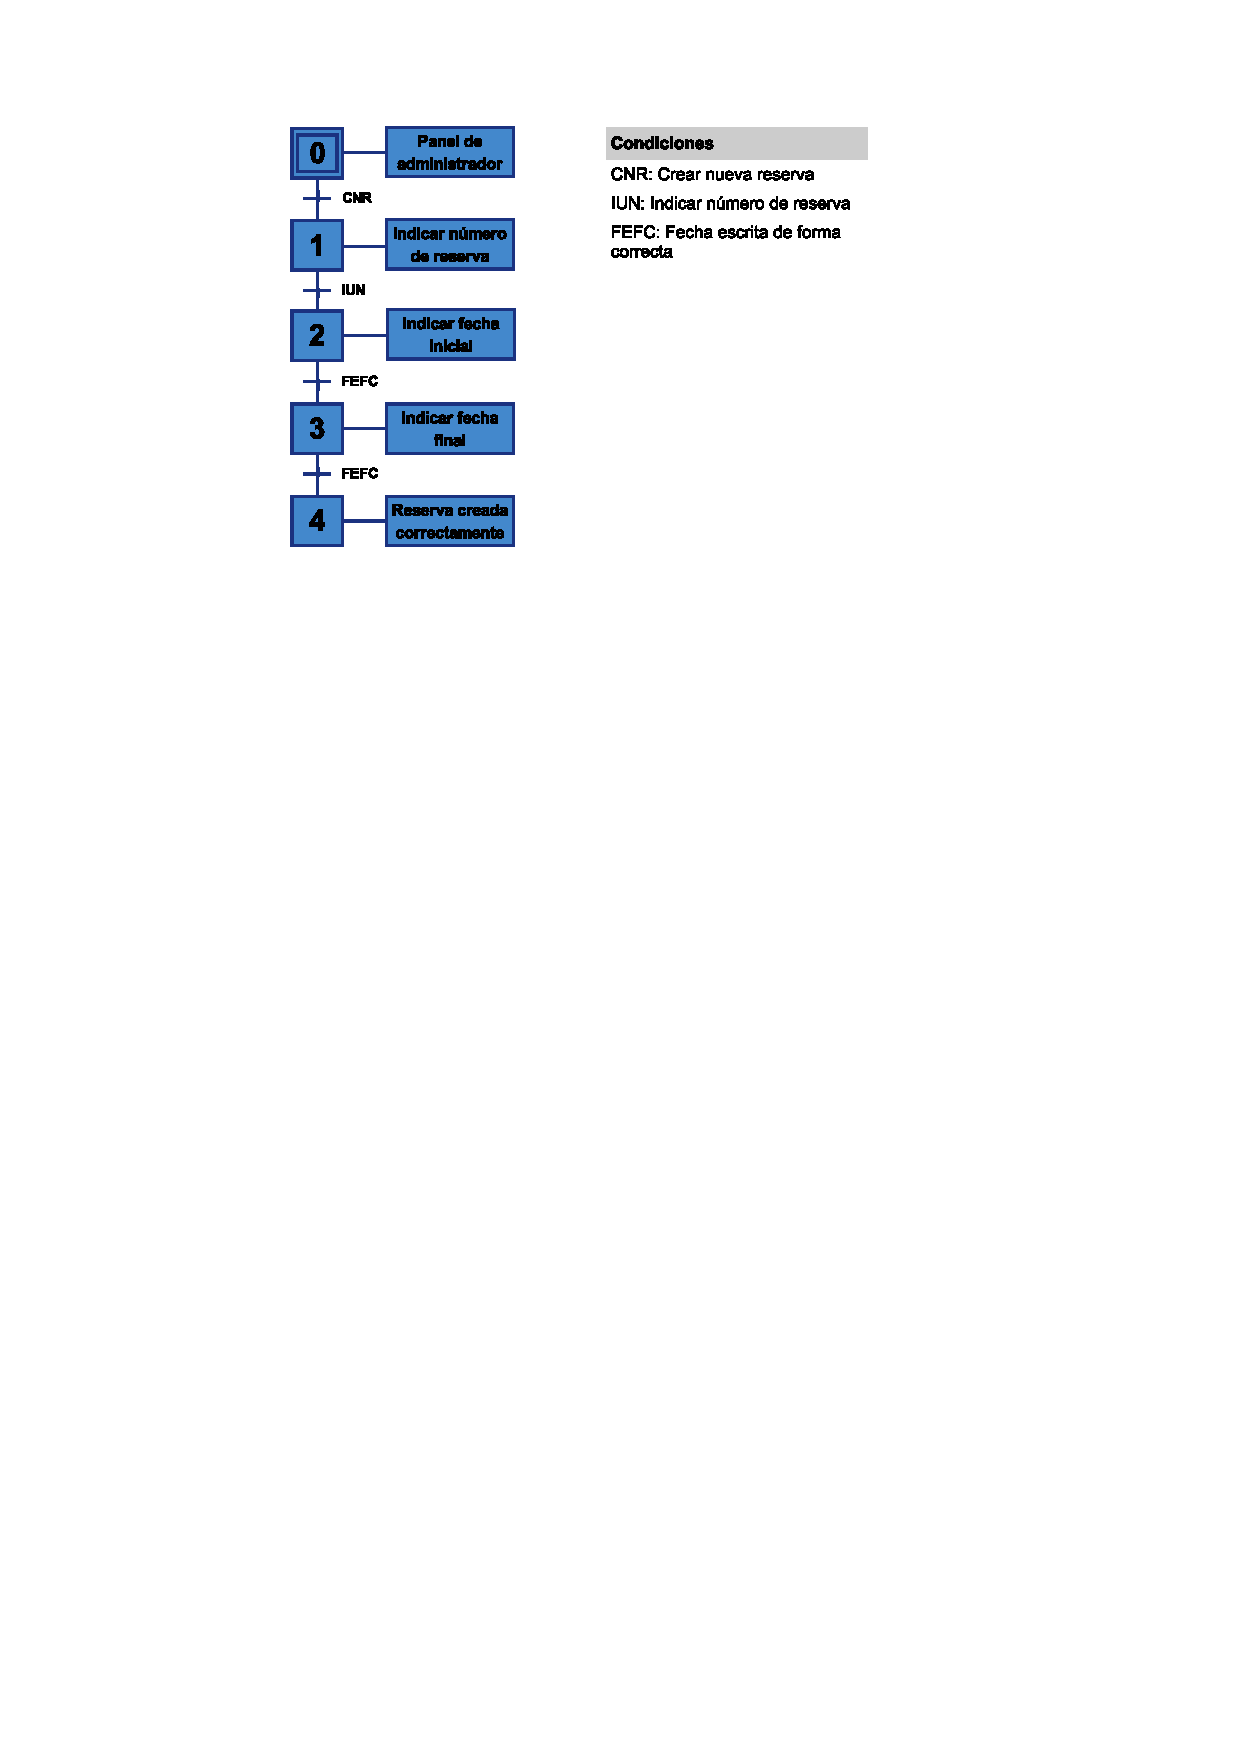
\includegraphics[scale=1]{fig/Grafcet_creacion_nueva_reserva.pdf}
\caption{Proceso de creación de una nueva reserva}
\label{fig:proceso-nueva-reserva}
\end{figure}

En dicho proceso puede observarse como el bot dirige al administrador durante la creación de una nueva reserva, permitiendo que esta se configure solo cuando se cumplen las condiciones necesarias que han sido definidas.
La primera condición debe ser que el administrador elija la opción de "Crear una nueva reserva", en cuyo caso, lo primero que hará el bot será pedirle un número de reserva. Este número de reserva será el que tendrá que usar aquella persona a la que este destinada la reserva para identificarse ante el bot y poder acceder a la vivienda. El número de reserva podrá estar compuesto por letras, números y otro tipo de caracteres.
Una vez introducido el número de reserva, el bot pedirá al administrador que le indique la fecha inicial. Para poder continuar a partir de este paso, es imprescindible que la fecha se introduzca en el orden que indica el bot (YYYY/MM/DD). En caso de que no se introduzca de esta manera, el bot no permitirá continuar con el proceso.
Habiendo indicado el número de reserva y la fecha inicial, solo quedará indicar la fecha final (con la misma condición que en el caso de la inicial) y el bot habrá dado por concluido el proceso de reserva.
Una vez que se ha indicado la fecha final, el archivo python almacena en el documento que almacena las reservas (reservas.txt), las variables de fecha y número de reserva.
El archivo mencionado "reservas.txt" será el encargado de ir almacenando cada una de las reservas creadas por parte del usuario, las cuales permanecerán a salvo a pesar de una interrupción en el funcionamiento de la Raspberry Pi.
Una vez que el proceso de reserva está listo, puede procederse a habilitar al bot para realizar la función de abrir la cerradura desde el panel de administrador.
\begin{lstlisting}[language=Python,
    caption={Apertura de puertas desde el panel de administración},
    label=src:apertura-puertas-panel-administrador
]
            elif a == "Abrir puerta":
                if paso2 == True or paso1 == True or paso3 == True:
                    paso1 = False
                    paso2 = False
                    paso3 = False
                bot.send_message(chatod, "Abriendo puerta...")
                blink()
\end{lstlisting}
El código que se aprecia en el listado 5.12 es el encargado de permitir el acceso a la vivienda por parte del administrador siempre que lo desee. Puede observarse que, para ello, se hace uso de la activación de la señal por medio de la función blink, explicada con anterioridad en el listado 5.7.
También se destaca como se desactivan todos los pasos correspondientes al proceso de reserva. Esto se realiza con el fin de que, si en mitad de una creación de reserva, el administrador decide abrir la puerta, el programa abriría pero se quedaría en el punto que estaba en esa función paralela, provocando errores en el futuro. Llevando a cabo esta acción se evita este error y se reinician desde el principio todas estas variables.

\begin{figure}[tbp]
\centering
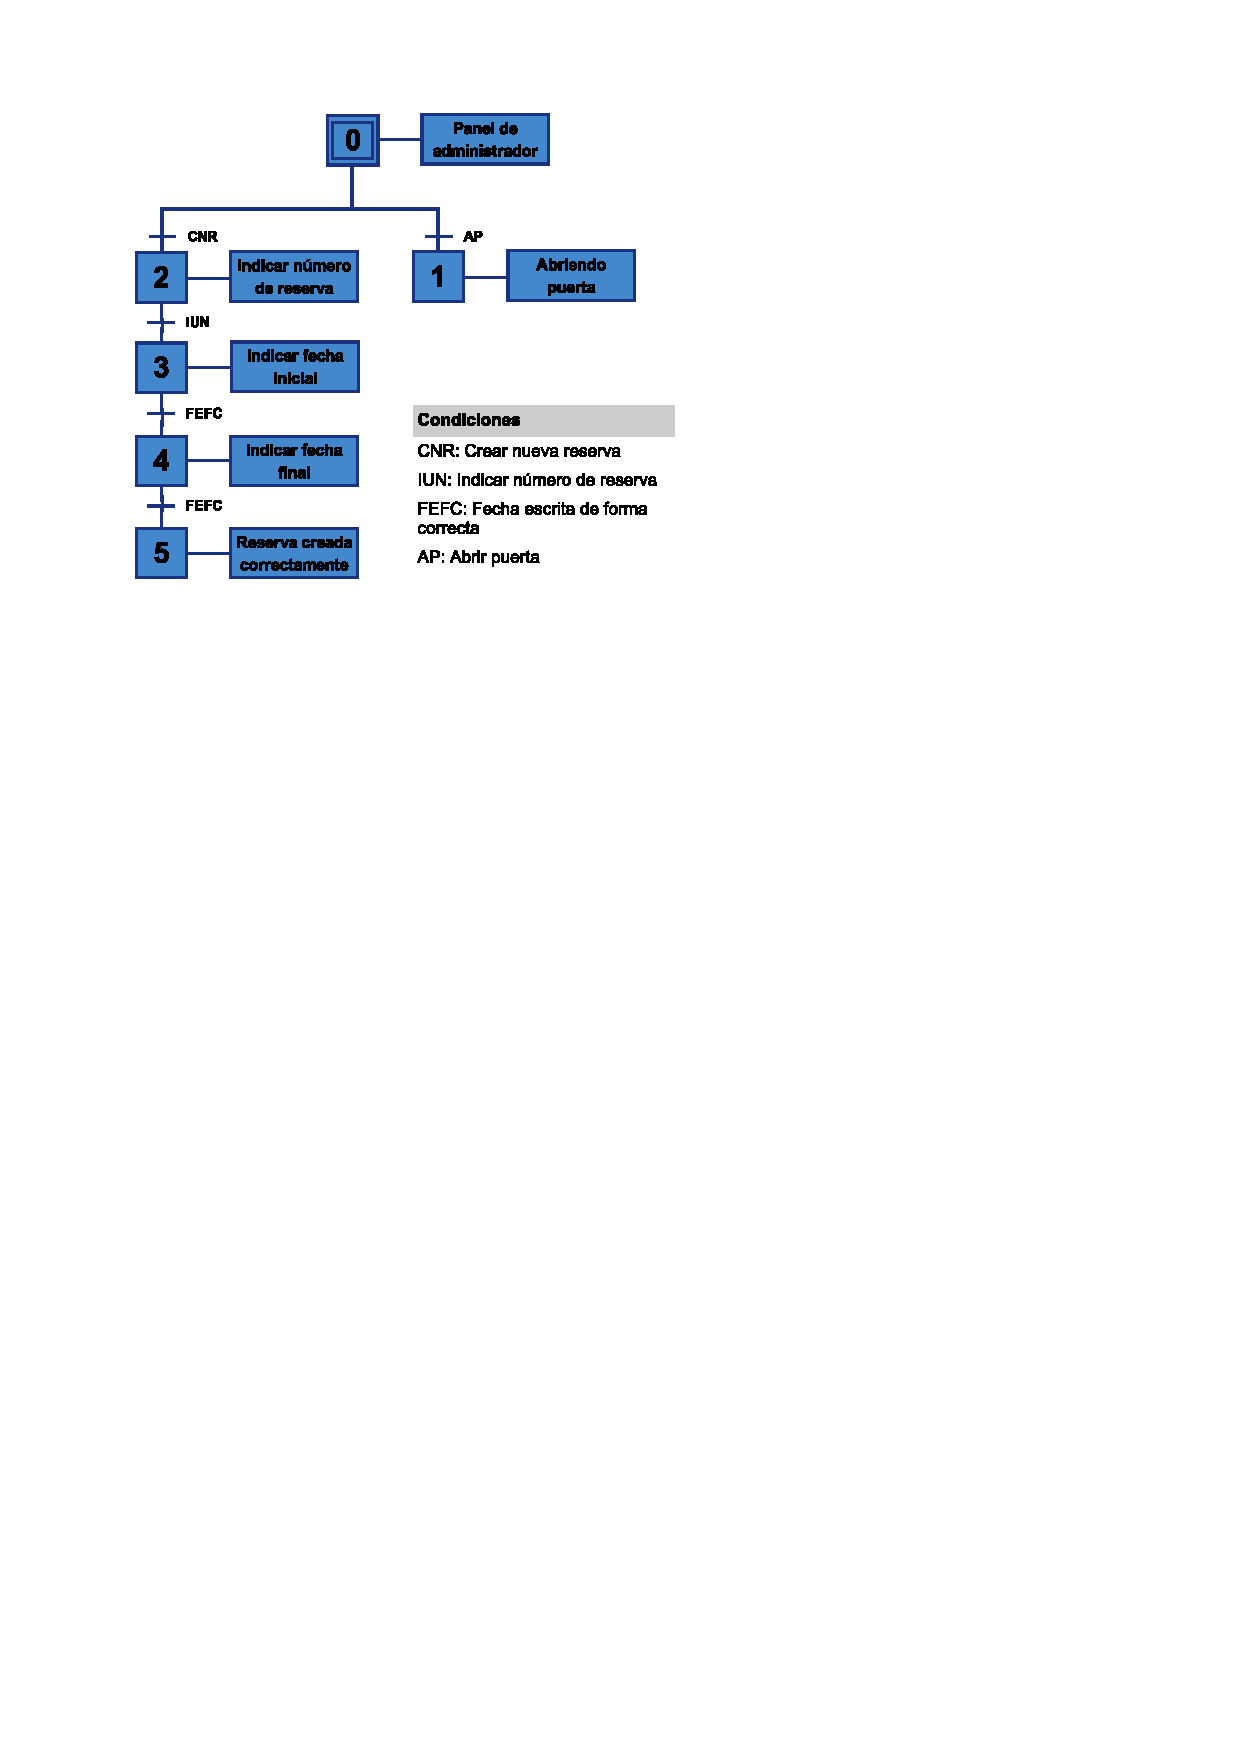
\includegraphics[scale=1]{fig/Grafcet_reserva_y_apertura.pdf}
\caption{Panel de administrador que permite crear reservas y realizar la apertura}
\label{fig:reserva-y-apertura}
\end{figure}

La siguiente opción que ha sido incluida en el panel de administrador es la de ofrecer la posibilidad de dejar de ser administrador. Esta opción puede llevarse a cabo por diferentes razones, como puede ser un administrador temporal (mientras el administrador principal está de vacaciones), para que el administrador principal pruebe el modo usuario, etc. Para conseguir que el bot desarrolle dicha opción, se ha incluido el código que se refleja en el listado 5.13:
\begin{lstlisting}[language=Python,
    caption={Dejar de ser administrador},
    label=src:dejar-de-ser-administrador
]
            elif a == "Dejar de ser administrador":
                if paso2 == True or paso1 == True or paso3 == True:
                    paso1 = False
                    paso2 = False
                    paso3 = False
                administradores.remove(chatod)
                bot.send_message(chatod, "Ya no tienes permisos de administrador")
\end{lstlisting}
En el extracto de código del listado 5.13 puede observarse, al igual que en casos anteriores, como antes de eliminar al usuario de administrador se procede a reinicializar todas las variables del proceso de reserva. Esto se hace con la intención de que no se quede ningún proceso a medias y que, cuando otro administrador trabaje en el bot, no se encuentre ninguna sorpresa.
Para eliminar al usuario como administrador de la propiedad, tan solo ha sido necesario eliminar su número de identificación del vector donde se almacenan los administradores. En la figura~\ref{fig:reserva-apertura-y-dejar-administracion} se muestra el algoritmo que describe el comportamiento del bot tras esta última actualización.
\begin{figure}[tbp]
\centering
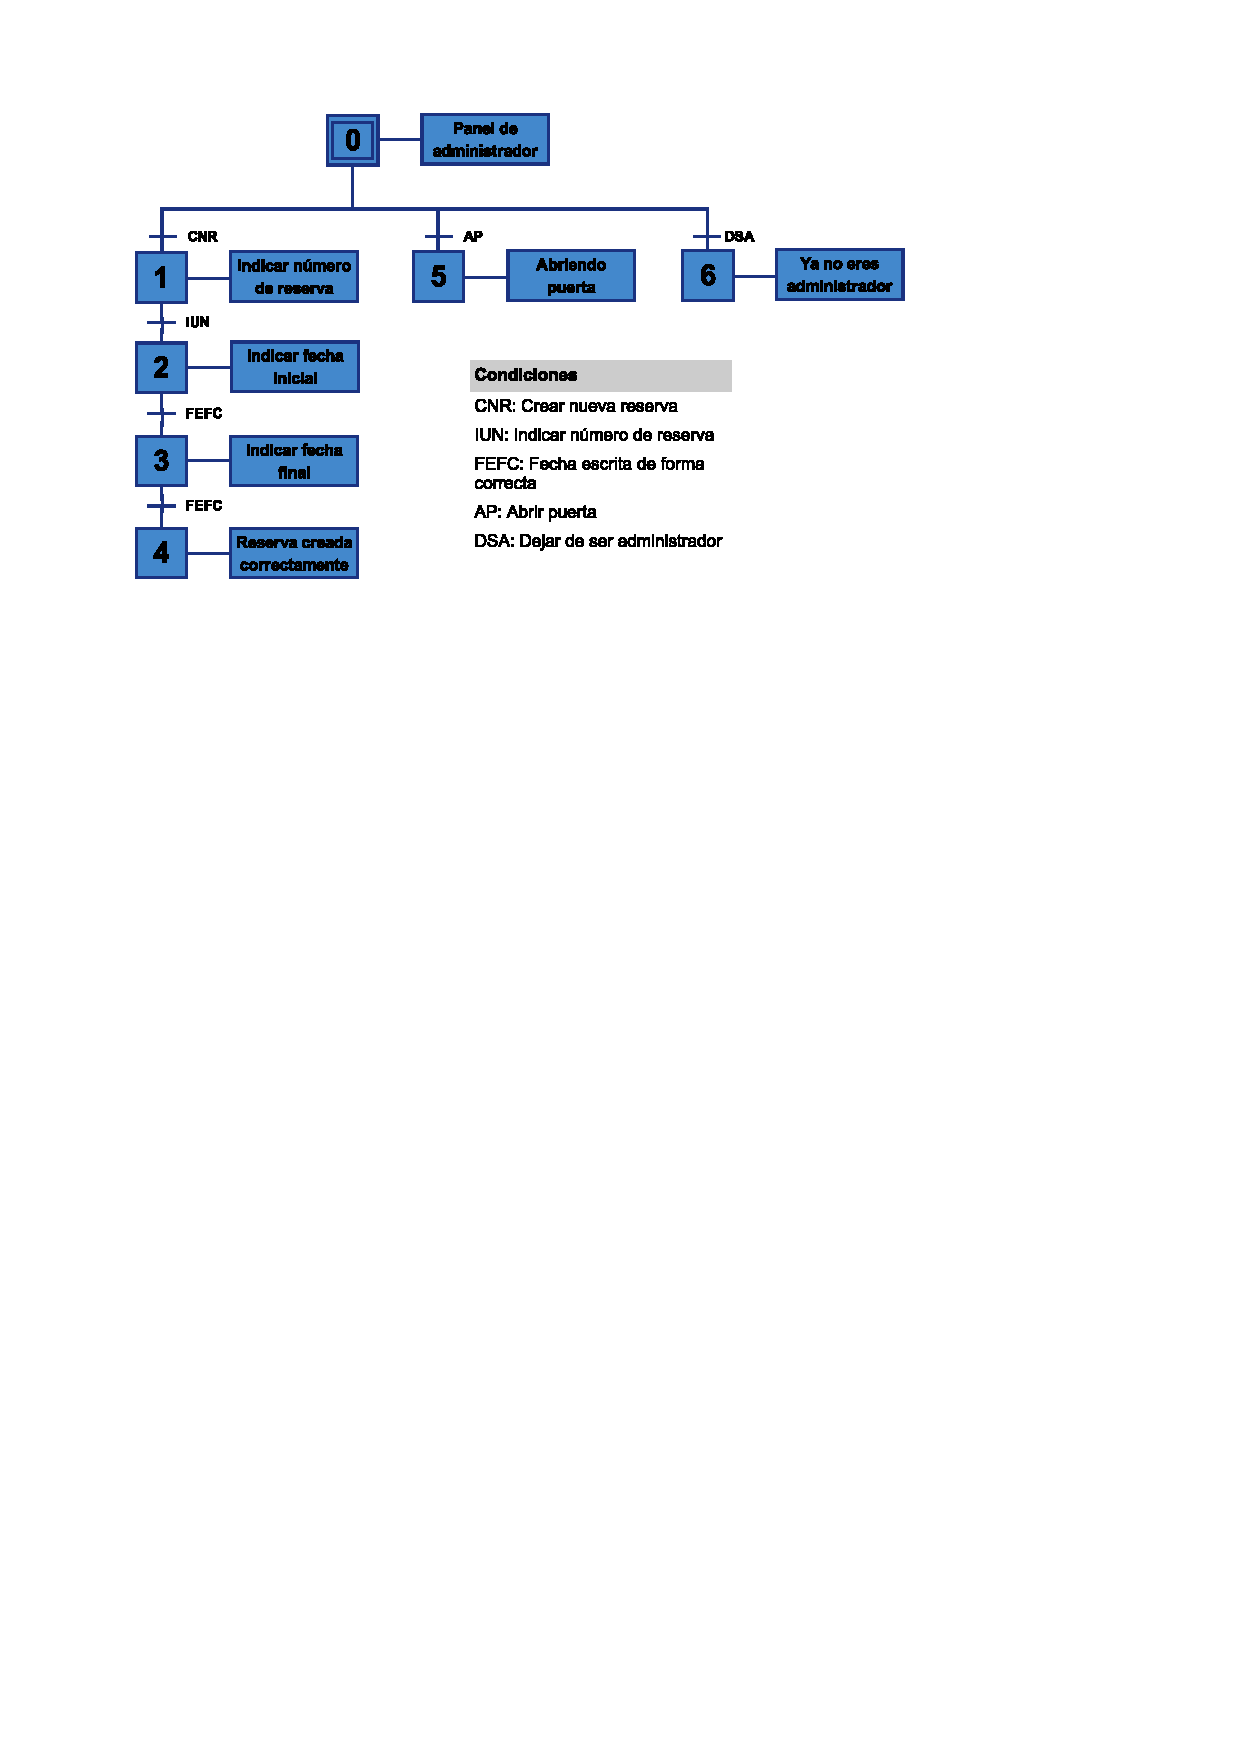
\includegraphics[scale=1]{fig/Grafcet_reserva_apertura_y_dejar_administracion.pdf}
\caption{Panel de administrador que permite crear reservas, realizar aperturas y dejar de ser administrador}
\label{fig:reserva-apertura-y-dejar-administracion}
\end{figure}
Atendiendo a los criterios que fueron definidos en el apartado de planificación del presente proyecto, solo faltaría añadir al panel de administrador la posibilidad de visualizar y/o modificar las reservas activas. El código que se muestra en el listado 5.14 es el encargado de llevar a cabo dicha tarea:
\begin{lstlisting}[language=Python,
    caption={Consulta y modificación de reservas},
    label=src:consulta-y-modificacion-de-reservas
]
                if paso2 == True or paso1 == True or paso3 == True:
                    paso1 = False
                    paso2 = False 
                reservas = ""
                tam = int(len(contrasenas))
                paso3 = True
                f = open ('reservas.txt','r')
                texto = f.read()
                f.close()
                vector = []
                if len(texto) > 0:
                    vector = convierteavector(texto)
                if len(vector)>0:
                    i = 0
                    while i < (len(vector)/4):
                        j=i+1
                        reservas = reservas + (""+str(j)+". Reserva para el día "+str(vector[i*4+2])+"-"+str(vector[i*4+1])+"-"+str(vector[i*4])+" con número de reserva: "+str(vector[i*4+3])+"\n")
                        i+=1
                    bot.send_message(chatod, reservas)
                    bot.send_message(chatod, "Si quieres eliminar alguna reserva, simplemente escribe el número que deseas eliminar")
                else:
                    bot.send_message(chatod, "No hay reservas activas")
            elif paso3 == True:
                paso3 == False
                f = open ('reservas.txt','r')
                texto = f.read()
                f.close()
                comprueba = compruebaentero(a)
                vector = convierteavector(texto)
                cantidad = (len(texto)/4)
                if comprueba == True:
                    if cantidad >= int(a):
                        a = int(a)
                        nr = a
                        a = (a - 1)*4
                        for i in range(4):
                            vector.pop(a)
                        f = open ('reservas.txt','w')
                        f.write(str(vector))
                        f.close()                                                 
                        bot.send_message(chatod, "Se ha borrado la reserva "+str(nr))
                    else:
                        bot.send_message(chatod, "El número no corresponde a ninguna reserva")
                else:
                    bot.send_message(chatod, "Lo siento, pero no entiendo el mensaje")
            else:
                bot.send_message(chatod, "No entiendo el mensaje")
\end{lstlisting}

Las líneas descritas en el listado 5.14 muestran el proceso que sigue el programa a la hora de realizar la consulta de reservas. Para realizar esta tarea de forma correcta, se deben tener en cuenta las dos opciones posibles en la consulta, donde la primera sería que haya reservas y en ese caso mostrarlas, y la segunda consistiría en que no haya reservas, y en ese caso transmitir esa información al administrador.

Solo en el caso de que haya reservas activas, se notificará al usuario la cantidad total de las mismas y se le ofrecerá la posibilidad de eliminar aquellas que desee, simplemente introduciendo el número correspondiente a dicha reserva.

El diagrama que se observa en la figura~\ref{fig:panel-administrador-completo} tiene por objeto mostrar, de forma más gráfica, el funcionamiento del panel de administrador que se ha dispuesto en el bot de Telegram.

\begin{figure}[tbp]
\centering
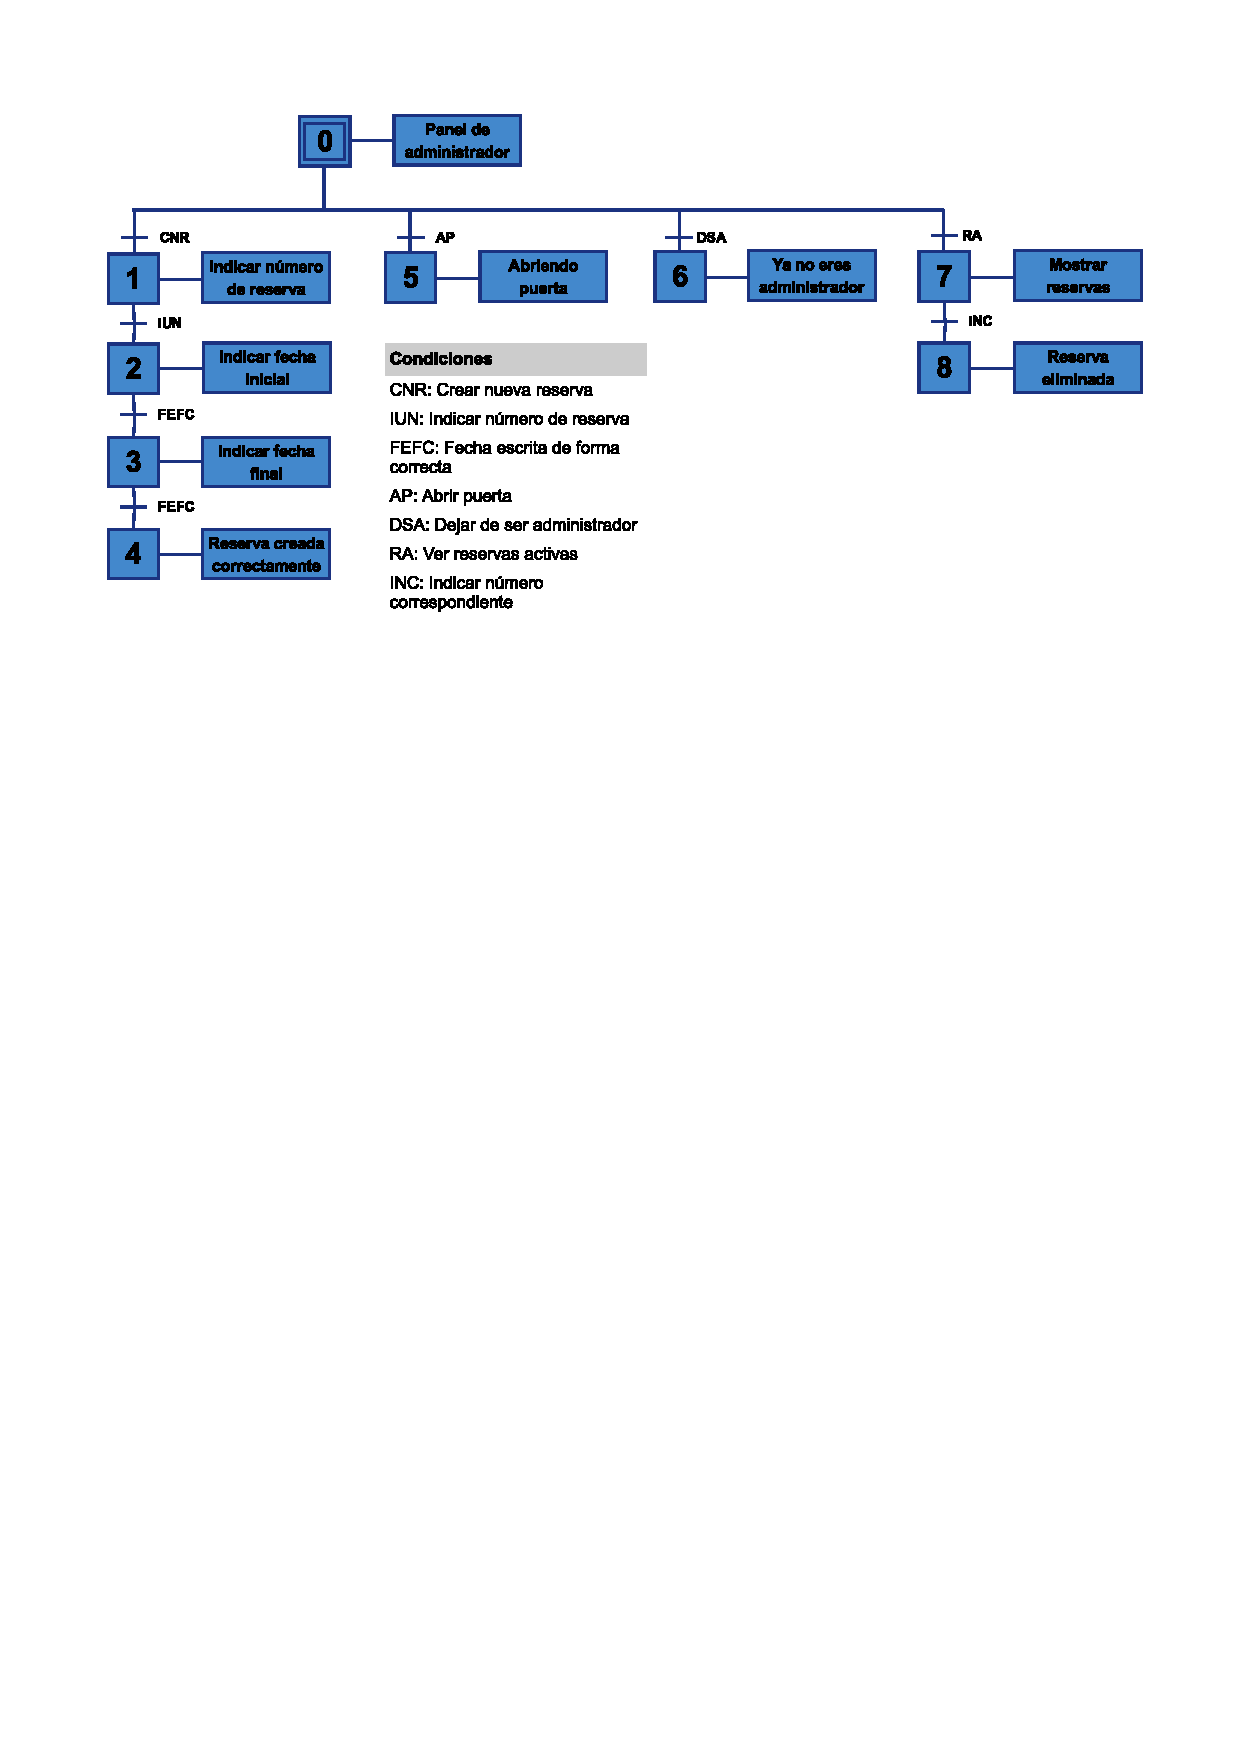
\includegraphics[scale=0.8]{fig/Panel_administrador_completo.pdf}
\caption{Panel de administrador completo}
\label{fig:panel-administrador-completo}
\end{figure}

Habiendo finalizado el proceso de consulta y modificación de reservas, se dan por completados todas las características previas que se definieron anteriormente sobre las opciones del administrador. Es momento, por tanto, de realizar la programación necesaria para autorizar la apertura de puertas a los usuarios finales.
Esta parte del código, a pesar de que se plantea de forma más sencilla que la anterior, debe tener en cuenta también diferentes factores y posibilidades distintas. Un usuario puede hacer una petición de apertura, pero para ello, se debe conocer primero si este usuario esta autorizado o no a llevar a cabo tal acción. Por ello, la primera parte de este código tendrá por objeto identificar si este usuario está activo, y en caso de que lo esté, comprobará si todavía está dentro de fecha para poder realizar aperturas.

En el caso de que el tiempo de estancia del huésped ya haya pasado, será eliminado de forma inmediata del vector de usuarios activos y se le anulará la posibilidad de realizar aperturas.
El código que se muestra en el listado 5.15 tiene por objeto hacer cumplir estas condiciones.

\begin{lstlisting}[language=Python,
    caption={Comprobar huéspedes activos},
    label=src:comprobar-huespedes-activos
]
        else:
            if paso3 == True or paso2 == True or paso1 == True:
                paso3 = False
                paso2 = False
                paso1 = False
            if chatod in usuariosactivos:
                posicion = int(usuariosactivos.index(chatod))
                fechamax = fechafinalusuario[posicion]
                comprobar = comprobarfechamaxima(fechamax)
                if comprobar == False:
                    usuariosactivos.remove(chatod)
                if chatod in usuariosactivos:                    
                    if a == "Abrir" or a == "abrir" or a == "Abrir puerta":            
                        bot.send_message(chatod, "Abriendo puerta...")
                        blink()                        
                    else:
                        bot.send_message(chatod, "Recuerda que para abrir solo necesitas escribir la palabra Abrir o pulsar el boton")
\end{lstlisting}

Puede observarse además, que el usuario tiene tres opciones distintas para realizar la apertura, escribiendo "abrir", "Abrir" o "Abrir puerta", y en caso de que no coincida con ninguna, se le enviarán instrucciones de como realizar la apertura.
Ahora debe tratarse la segunda posibilidad, que sería aquella en la que el usuario todavía no se ha registrado como huésped, y por tanto, debe identificarse para que el bot pueda definir correctamente si este tiene o no permisos de apertura.

Para realizar esta operación de forma correcta, será necesario consultar las reservas activas a través del documento reservas.txt, y en caso de que el número de reserva indicado por el usuario sea correcto, se deberá verificar que se encuentra dentro de plazo. Esta operación se realiza a través del código que se observa en el listado 5.16.
\begin{lstlisting}[language=Python,
    caption={Registrar nuevo huesped},
    label=src:registrar-nuevo-huesped
]
            else:
                f = open ('reservas.txt','r')
                texto = f.read()
                f.close()
                vector = convierteavector(texto)
                if a in vector:
                        posicion=vector.index(a)
                        fechainic=(""+vector[posicion-3]+"-"+vector[posicion-2]+"-"+vector[posicion-1])
                        fechafin = datetime.strptime(fechainic, '%Y-%m-%d')
                        fechafin = fechafin + timedelta(days=1)
                        fechafin = str(fechafin)
                        verificafechainic=comprobarfecha(fechainic)
                        verificafechafin=comprobarfechamaxima(fechafin)
                        if verificafechainic==True and verificafechafin==True:                            
                            mensajetipo="Enhorabuena! Ya puedes acceder a tu vivienda pulsando o escribiendo Abrir. Espero que tengas una gran estancia"
                            markup=types.ReplyKeyboardMarkup()
                            markup.add('Abrir puerta')
                            usuariosactivos.append(chatod)
                            fechafinalusuario.append(chatod)
                            bot.send_message(chatod, mensajetipo, None, None, markup)     
                        else:
                            bot.send_message(chatod, "Su reserva está fuera de fecha, recuerda que esta reserva corresponde al periodo del "+fechainic+"a las 12:00 hasta "+fechafin+" a las 15:00")
\end{lstlisting}
Con esto quedaría definido el papel del usuario final en este programa, tanto en caso de estar registrado, como en el de necesitar su registro en la plataforma.
No obstante, para evitar que, de forma malintencionada, se intente desbloquear el acceso a la vivienda introduciendo miles de números distintos por medio de un ordenador, se ha limitado la posibilidad de equivocarse con el número de reserva a 50 veces. En el código que se muestra a continuación, se puede observar como al alcanzar dicha cifra, el usuario queda registrado en una lista negra que, atendiendo al condicional de la línea 7 en el listado 4.9, no permitirá que pueda seguir intentando acceder a la vivienda. En el listado 5.17 se muestra el código que realiza dicha tarea.
\begin{lstlisting}[language=Python,
    caption={Limitación de intentos para acceder a la vivienda},
    label=src:limite-de-intentos
]
                else:                    
                    bot.send_message(chatod, "El número de reserva que has introducido no es correcto, por favor, inténtelo de nuevo")
                    if chatod in contador_intentos_erroneos:
                        if intentos == 50:
                            listanegra.append(chatod)
                        else:
                            posicion = contador_intentos_erroneos.index(chatod)
                            posicion += 1
                            intentos = contador_intentos_erroneos[posicion]
                            intentos+=1
                            contador_intentos_erroneos[posicion] = intentos
\end{lstlisting}
Una vez llevada a cabo esta acción, el programa central, que tiene por objeto realizar la interacción con los usuarios y el administrador, queda definido correctamente.
Es momento de hacer que, tanto las reservas, como las cancelaciones, se incluyan o excluyan del documento "reservas.txt" del cual recoge la información el programa central.
Para ello, se ejecutará otro programa en paralelo, que tendrá por objeto llevar a cabo la labor de tener en cuenta las reservas y las cancelaciones. Este programa contará con la importación de algunas librerías, tal como puede observarse en el código 5.18.
\begin{lstlisting}[language=Python,
    caption={Importación de librerias para programa de reservas y cancelaciones},
    label=src:importacion-librerias-reservas-y-cancelaciones
]
import time
from itertools import chain
import email
import imaplib
import string
\end{lstlisting}
En este programa se va a trabajar con un correo de gmail. Esto se ha decidido así, ya que gmail es un correo electrónico muy popular en España, y será por tanto, el que más administradores de viviendas utilizarán. No obstante, las librerías importadas permitirían trabajar con cualquier proveedor, como yahoo, hotmail, etc.
Si se observa el listado 5.19, puede verse el proceso que se realiza con el fin de establecer la configuración pertinente que será necesaria para conectar con el correo de gmail.com:
\begin{lstlisting}[language=Python,
    caption={Configuración de gmail},
    label=src:configuracion-de-gmail
]
imap_ssl_host = 'imap.gmail.com'
imap_ssl_port = 993
username = 'correoadministrador@dominio'
password = 'Contrasenacorreo'
criterios-busqueda = {
    'FROM':    'correo_remitente_booking',
    'SUBJECT': 'Aquí se incluye el asunto del correo',
    'BODY':    'Nombre de la vivienda de uso turístico',
}
\end{lstlisting}
En el extracto de código del listado 5.19 puede observarse un apartado llamado "criterios-busqueda". Este apartado tiene por objeto definir aquellos criterios en los que se fijará a la hora de buscar un correo electrónico u otro. Para no trabajar correos que no tengan nada que ver con las viviendas de uso turístico, se puede definir en el subapartado "from" que solo se atenderán aquellos correos provenientes de booking.com, por ejemplo. O se puede incluir en el cuerpo del mensaje el nombre del apartamento, de manera que solo se busquen correos relacionados con ese tema.
A partir de la función que se define en el listado 5.20, se procederá a realizar la búsqueda de aquellos correos que cumplan con los criterios de búsqueda especificados en el punto anterior:
\begin{lstlisting}[language=Python,
    caption={Búsqueda de correos de reservas o cancelaciones},
    label=src:busqueda-de-correos
]
def search_string(uid_max, criterios-busqueda):
    c = list(map(lambda t: (t[0], '"'+str(t[1])+'"'), criterios-busqueda.items())) + [('UID', '%d:*' % (uid_max+1))]
    return '(%s)' % ' '.join(chain(*c))
}
\end{lstlisting}
También será necesaria una función que se encargue de extraer el bloque de texto de cada correo. En el listado 5.21 se lleva a cabo la definición de dicha función.
\begin{lstlisting}[language=Python,
    caption={Extracción de texto del correo},
    label=src:extraccion-del-texto-del-correo
]
def get_first_text_block(msg):
    type = msg.get_content_maintype()
    if type == 'multipart':
        for part in msg.get_payload():
            if part.get_content_maintype() == 'text':
                return part.get_payload()
    elif type == 'text':
        return msg.get_payload()
\end{lstlisting}
Una vez definidas las funciones, se procede a la creación de un código que reciba las nuevas reservas y cancelaciones, y actualice el sistema en coherencia. El código elaborado para tal efecto está definido de forma integral en el listado 5.22.
\begin{lstlisting}[language=Python,
    caption={Recepción de reservas y cancelaciones},
    label=src:recepcion-de-reservas-y-cancelaciones
]
server = imaplib.IMAP4_SSL(imap_ssl_host, imap_ssl_port)
server.login(username, password)
server.select('INBOX')
result, data = server.uid('search', None, search_string(uid_max, criterios-busqueda))
uids = [int(s) for s in data[0].split()]
if uids:
    uid_max = max(uids)
server.logout()
while 1:
    server = imaplib.IMAP4_SSL(imap_ssl_host, imap_ssl_port)
    server.login(username, password)
    server.select('INBOX')
    result, data = server.uid('search', None, search_string(uid_max, criterios-busqueda))
    uids = [int(s) for s in data[0].split()]
    for uid in uids:
        if uid > uid_max:
            result, data = server.uid('fetch', uid, '(RFC822)')
            msg = email.message_from_string(data[0][1])            
            uid_max = uid     
            text = get_first_text_block(msg)
            print 'New message :::::::::::::::::::::'
            buscareserva = str(msg)
            if "t_new_reservation" in buscareserva:                
                pos = buscareserva.index("t_new_reservation")
                pos = pos + 21
                posfinal = pos + 10
                numreserva = buscareserva[pos:posfinal]
                print ("El numero de reserva es el "+numreserva)
                print("es reserva")
            if "Cancelaci" in buscareserva:
                pos = buscareserva.index("res_id=")
                pos = pos + 9
                posfinal = pos + 10
                numreserva = buscareserva[pos:posfinal]
                print ("El numero de cancelacion es el "+numreserva)
            for i in range(200):
                ano = str(anos[i])
                if (" de "+ano+")") in buscareserva:
                    pos = buscareserva.index((" de "+ano+")"))
                    posfinal = pos + 8
                    bucleinf = True
                    while bucleinf == True:
                        pos = pos - 1
                        if buscareserva[pos] == ",":
                            bucleinf = False
                    pos = pos + 2
                    buscafecha = buscareserva[pos:posfinal]
                    buscafecha = buscafecha.split(' de ')
                    buscafecha = conviertefecha(buscafecha)
                    buscafecha.append(numreserva)
                    f = open ('reservas.txt','r')
                    texto = f.read()
                    f.close()
                    if len(texto) > 0:
                        vector = convierteavector(texto)
                    if "Cancelaci" in buscareserva:
                        if numreserva in vector:
                            pos = vector.index(numreserva)
                            pos = pos -3
                            for i in range(4):
                                vector.pop(pos)
                                print(vector)
                    else:
                        for i in range(4):
                            vector.append(buscafecha[i])
                    f = open ('reservas.txt','w')
                    f.write(str(vector))
                    f.close()          
    server.logout()
    time.sleep(1)
\end{lstlisting}
Para realizar de forma correcta la clasificación de reservas y cancelaciones, se ha decidido analizar el contenido de cada correo recibido. Para ello, se convierte la información en una cadena de texto con la que poder trabajar y se ha estudiado, por medio de diferentes correos reales de Booking.com, las coincidencias que aparecen siempre. El fin es extraer, a partir de esa información, los datos necesarios para crear las reservas y las cancelaciones.
Cada correo, dependiendo de si es una cancelación o una reserva, tiene unas características particulares que permiten diferenciarlo a nivel de código. Una vez que se sabe que tipo de correo es el recibido, y que se extrae la información de número de reserva y fecha, tan solo queda guardarla en el archivo "reservas.txt" compartido con el programa central realizado al comienzo de esta sección.
\subsection{Seguridad del dispositivo}
Aunque esta sección trata de forma específica las medidas de seguridad que se han considerado integrar en el prototipo, la seguridad es un aspecto que se ha tenido en cuenta a lo largo de todo el proyecto.
Se pueden encontrar muchas razones, a todos los niveles, por las cuales crear un dispositivo seguro:
\begin{itemize}
\item{Proporcionará a los anfitriones la garantía de que su vivienda se encuentra protegida, fomentando así el uso de esta herramienta.}
\item{Los usuarios tendrán la garantía de que el sistema no les dejará abandonados en ningún momento, generando así confianza en los mismos.}
\item{Fomentará la confianza en posibles inversores que quieran interesarse por el producto, al ver que se han tenido en cuenta las diferentes situaciones problemáticas que pueden surgir de forma natural.}
\end{itemize}
Estas son solo algunas de las razones por las cuales este punto es uno de los más importantes en el desarrollo de este trabajo de fin de grado. La seguridad debe ir dirigida, no solo a la defensa ante posibles ataques externos, si no también al hecho de responder ante posibles fallos del propio sistema que no hayan sido identificados con anterioridad.

En la planificación del proyecto se establecen los pasos a seguir en cuanto a la seguridad del dispositivo, por lo que a continuación se describen las tareas realizadas en cada uno de dichos pasos:

El primer punto que se trataba en el apartado 1.2.3, referido a las tareas orientadas a la seguridad del dispositivo, era el de crear un programa capaz de prevenir manipulaciones malintencionadas. Para ello, la solución que se ha propuesto es la de incluir un sistema que sea capaz de avisar al usuario en el caso de que alguien abra la caja donde se encuentra el dispositivo. 

Para llevar a efecto dicha propuesta, se ha hecho uso de un sensor de ultrasonidos, modelo HC-SR04, el cual puede observarse en la figura~\ref{fig:sensor-detector-distancia} y permite obtener en todo momento la distancia a la que se encuentra un objeto. En este caso, la distancia que se medirá será la tapa de la caja, de manera que, en el momento en el que aumente, se dará por hecho que la caja ha sido abierta. Al detectarse dicha situación, el mismo software que controla el sensor será el encargado de enviar un correo electrónico al anfitrión, avisándole de lo ocurrido, con el fin de que pueda tomar las medidas pertinentes.

\begin{figure}[tbp]
\centering
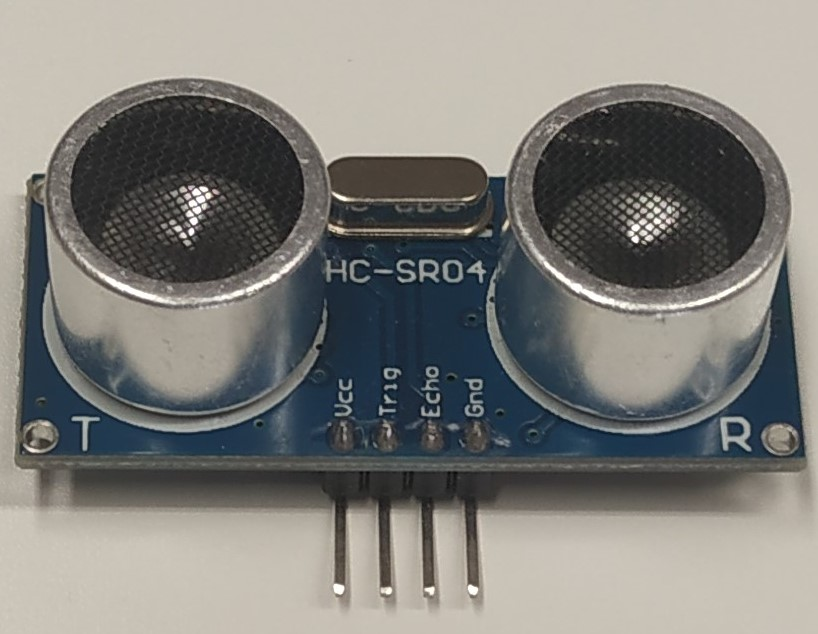
\includegraphics[height=4.5cm]{fig/Sensor-HC-SR04.jpg}
\caption{Sensor de distancia modelo HC-SR04}
\label{fig:sensor-detector-distancia}
\end{figure}

En el listado 5.23 se puede observar el código definido para realizar las tareas mencionadas.

\begin{lstlisting}[language=Python,
    caption={Alarma ante posibles manipulaciones},
    label=src:alarma-ante-posibles-manipulaciones
]
import RPi.GPIO as GPIO
import time
import smtplib
from email.mime.text import MIMEText
from email.mime.multipart import MIMEMultipart
GPIO.setmode(GPIO.BCM)
GPIO_TRIGGER = 17        
GPIO_ECHO    = 4      
GPIO.setup(GPIO_TRIGGER,GPIO.OUT) 
GPIO.setup(GPIO_ECHO,GPIO.IN)  
GPIO.output(GPIO_TRIGGER,False) 
destinatario = "correo del anfitrion"
def alarma(destinatario):   
    mailServer = smtplib.SMTP('smtp.gmail.com',587)
    mailServer.ehlo()
    mailServer.starttls()
    mailServer.ehlo()
    mailServer.login("correoremitente","contr_correo_remitente")
    print (mailServer.ehlo())
    mensaje = MIMEMultipart()
    mensaje['From']="correo_remitente"
    mensaje['To']=destinatario
    mensaje['Subject']="Atencion: la caja ha sido abierta"
    # Adjuntamos el texto
    mensaje.attach(MIMEText("Por seguridad, te avisamos de que alguien ha abierto la caja de tu dispositivo Keyhome."))
    mailServer.sendmail("keyhomeproject@gmail.com",
                    destinatario,
                    mensaje.as_string())
    mailServer.close()
try:
    while True:
        GPIO.output(GPIO_TRIGGER,True)
        time.sleep(0.001)
        GPIO.output(GPIO_TRIGGER,False)
        start = time.time()  
        while GPIO.input(GPIO_ECHO)==0:
            start = time.time() 
        while GPIO.input(GPIO_ECHO)==1: 
            stop = time.time()       
        elapsed = stop-start     
        distance = (elapsed * 34300)/2  
        print (distance)  
        if distance > 5:
            alarma(destinatario)
            break
        time.sleep(1)
except KeyboardInterrupt:
    print ("sesion finalizada")
    GPIO.cleanup()
\end{lstlisting}

En el código del listado 5.23 puede observarse la coordinación de dos tareas independientes. En primer lugar, se define una función que envía un correo electrónico al administrador avisándole de una posible manipulación, y en segundo lugar, se ejecuta un programa que mide en todo momento la distancia con el sensor de proximidad, realizando un condicional para que en caso de que la distancia aumente de 5cm, se active la función definida anteriormente que avisará al administrador.

Para alcanzar un resultado óptimo en lo relativo a la seguridad del dispositivo, se continúa con las tareas programadas, integrando un programa que avise al anfitrión en caso de una interrupción sobre el correcto funcionamiento del dispositivo. La función principal que desarrollará esta aplicación integrada, será la de avisar al anfitrión si cualquiera de los programas que actúan en conjunto deja de funcionar.

Para llevar a efecto tal misión, se ha hecho uso de un repositorio de Github\footnote{\url{https://github.com/initialstate/pi-process-dashboard/wiki}}, el cuál permite, a través de la integración de ciertos programas en la Raspberry Pi, monitorizar el funcionamiento de aquellos que se encuentran en ejecución.

La primera tarea a llevar a cabo será la de crear un programa que permita realizar la monitorización de la aplicación central que realiza la apertura de las puertas. Para ello, lo primero que se hace es registrarse en la plataforma\footnote{\url{https://iot.app.initialstate.com/}} que ofrecen en el propio repositorio, donde se obtienen una serie de claves, necesarias para la ejecución del programa.

Una vez realizada dicha acción, se procede a crear un archivo de python que contenga el código que se indica en listado 5.24.

\begin{lstlisting}[language=Python,
    caption={Monitorización de un proceso},
    label=src:monitorizacion-de-un-proceso
]
import psutil
import time
import sys
from ISStreamer.Streamer import Streamer
from subprocess import PIPE, Popen
BUCKET_NAME  =  " :Nombre_Monitorizacion" 
BUCKET_KEY  =  "pr1208"
ACCESS_KEY  =  "CLAVE DE ACCESO OBTENIDA"
PROCESS_NAME =  "PONGA EL NOMBRE DE SU PROCESO AQUI" 
MINUTES_BETWEEN_READS  =  1
def main():
	if len(sys.argv) != 2:
		print "Usage: " + sys.argv[0] + " <pid>"
		exit()
	pid = sys.argv[1]
	streamer = Streamer(bucket_name=BUCKET_NAME, bucket_key=BUCKET_KEY, access_key=ACCESS_KEY)
	if psutil.pid_exists(int(pid)) == False:
		print "Error: That process doesn't exist! Exiting ..."
		exit()
	else:
		streamer.log(PROCESS_NAME,"Running")
		streamer.flush()

	while True:
		if psutil.pid_exists(int(pid)) == False:
			streamer.log(PROCESS_NAME,"Exited")
			streamer.flush()
			exit()
		else:
			streamer.log(PROCESS_NAME,"Running")
			process = Popen(['hostname', '-I'], stdout=PIPE)
			output, _error = process.communicate()
			streamer.log(PROCESS_NAME + " IP Address", output.rstrip())
			streamer.flush()
		time.sleep(60*MINUTES_BETWEEN_READS)

if __name__ == "__main__":
    main()
}
\end{lstlisting}

La siguiente acción a realizar se basa en el lenguaje Bash, a través de un archivo de extensión .sh, que será el encargado de encontrar el PID (Process ID) o identificación del proceso que se pretende analizar. Una vez que se disponga de esta identificación, hará que se ejecute el programa de monitorización. El archivo de extensión .sh que se creará, será tal como se observa en el listado 5.25.

\begin{lstlisting}[language=Bash,
    caption={Monitorización de un proceso en archivo .sh},
    label=src:monitorizacion-de-un-proceso-en-archivo-sh
]
PROGRAMA_A_MONITORIZAR = "Ruta hacia el programa que se pretende monitorizar" 
PROGRAMA_QUE_MONITORIZA = "Ruta hacia el programa creado anteriormente para monitorizar" 
nohup $ PROGRAMA_A_MONITORIZAR  & 
VAR = ` pgrep -f " $ PROGRAMA_QUE_MONITORIZA " `
 echo  $ VAR 
nohup python $ MONITOR_SCRIPT  $ VAR  &
\end{lstlisting}

Al haber completado esta acción, solo queda definir en que momentos se pretende crear un aviso hacia el anfitrión de la vivienda. En este caso, con el fin de informar ante posibles interrupciones del funcionamiento, se avisará al anfitrión en los siguientes casos:
\begin{itemize}
\item{En el caso de que el programa encargado de realizar la apertura de puertas deje de estar operativo.}
\item{En el caso de que el programa encargado de atender las nuevas reservas y cancelaciones deje de estar operativo.}
\item{En el caso de que el programa encargado de avisar ante posibles manipulaciones deje de estar operativo.}
\end{itemize}

Para recibir estos avisos, es necesario acceder a la plataforma de InitialState\footnote{\url{https://iot.app.initialstate.com/}}, donde se permite crear avisos personalizados, tal como puede observarse en la figura~\ref{fig:aviso-personalizado}.

\begin{figure}[tbp]
\centering
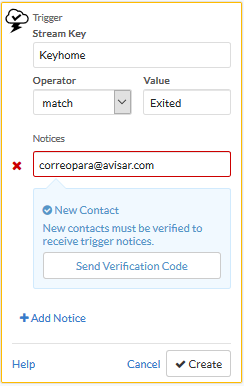
\includegraphics[scale = 0.8]{fig/Configuracion-de-aviso.PNG}
\caption{Configuración de aviso en la plataforma InitialState}
\label{fig:aviso-personalizado}
\end{figure}

En la figura~\ref{fig:sensor-detector-distancia} puede observarse como se crea un aviso, en el caso de que en la monitorización llamada Keyhome, se produzca una interrupción del funcionamiento (Exited), se informará del suceso al correo que se indica. De esta manera, el anfitrión tendrá la seguridad, en todo momento, de que su sistema se encuentra en funcionamiento, y de que, en caso de que algún programa falle, tendrá conocimiento de ello y podrá actuar en consecuencia.

Una vez que todas las debilidades tenidas en cuenta han sido consideradas a nivel de software, llega el momento de realizar un diseño que convierta este proyecto en un prototipo también a nivel físico. Para ello, se ha llevado a cabo el desarrollo de una caja donde se almacenará el circuito electrónico que incluye la Raspberry Pi, el sensor de proximidad, el conversor de niveles lógicos y el relé.

Para llevar a cabo el diseño de este prototipo, se ha hecho uso de la aplicación Autodesk Fusion 360\footnote{\url{https://www.autodesk.com/products/fusion-360/overview}}, la cual permite realizar diseños en tres dimensiones que posteriormente pueden ser impresos.

La función de este dispositivo es, principalmente, garantizar los niveles mínimos de seguridad a nivel físico, evitando que la Raspberry Pi o cualquier otro elemento pueda ser manipulado. Además, esta proporciona un mayor atractivo visual al dispositivo, haciendo que resulte más llamativo a nivel comercial.

En las figuras ~\ref{fig:imagen-1-diseno-3d}, ~\ref{fig:imagen-2-diseno-3d}, ~\ref{fig:imagen-3-diseno-3d}, ~\ref{fig:imagen-4-diseno-3d} y ~\ref{fig:imagen-5-diseno-3d} puede observarse, en distintos ángulos, el aspecto físico que se ha proporcionado a este dispositivo.

\begin{figure}[tbp]
\centering
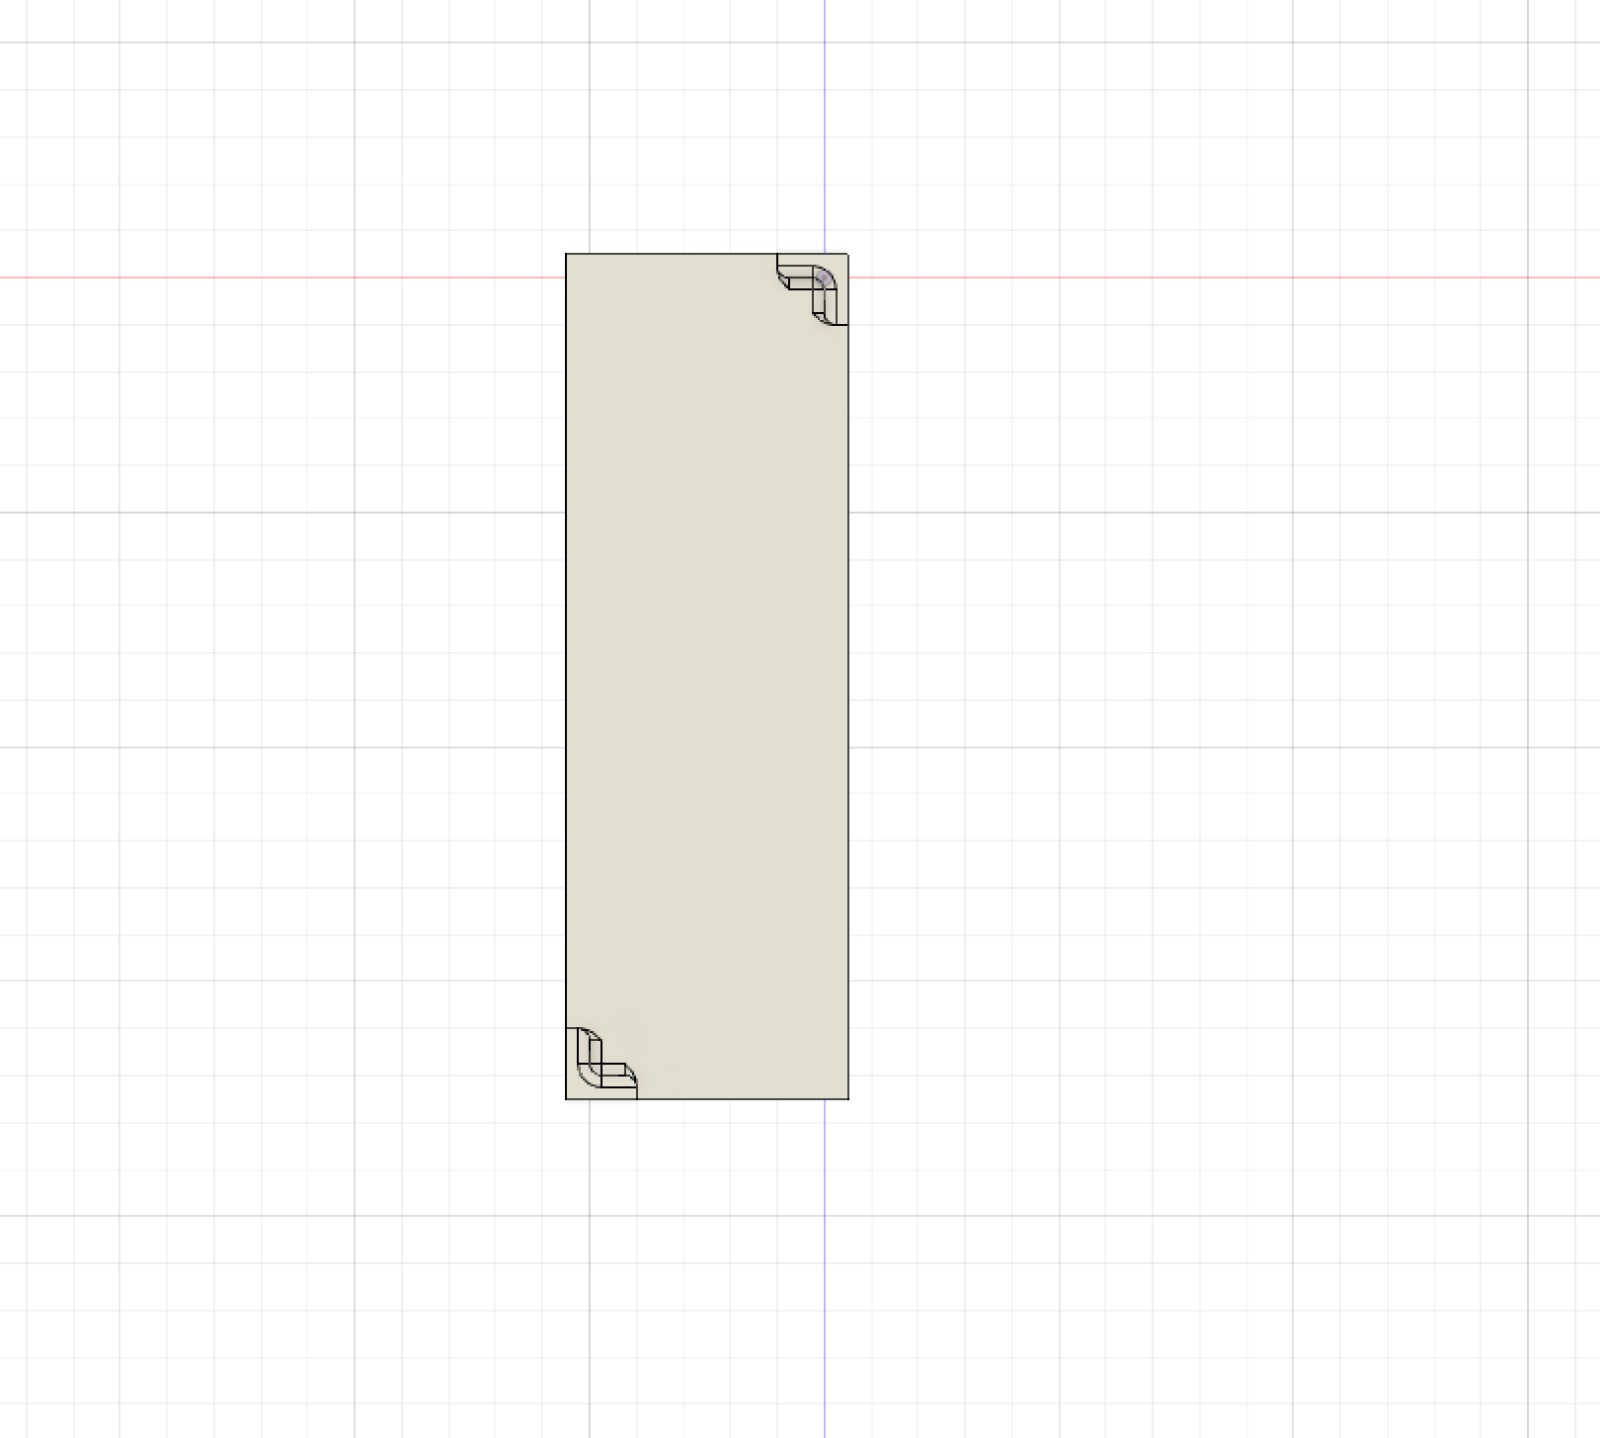
\includegraphics[scale = 0.2]{fig/Imagen_1_diseno_3D.jpeg}
\caption{Imagen 1 del diseño en 3D}
\label{fig:imagen-1-diseno-3d}
\end{figure}

\begin{figure}[tbp]
\centering
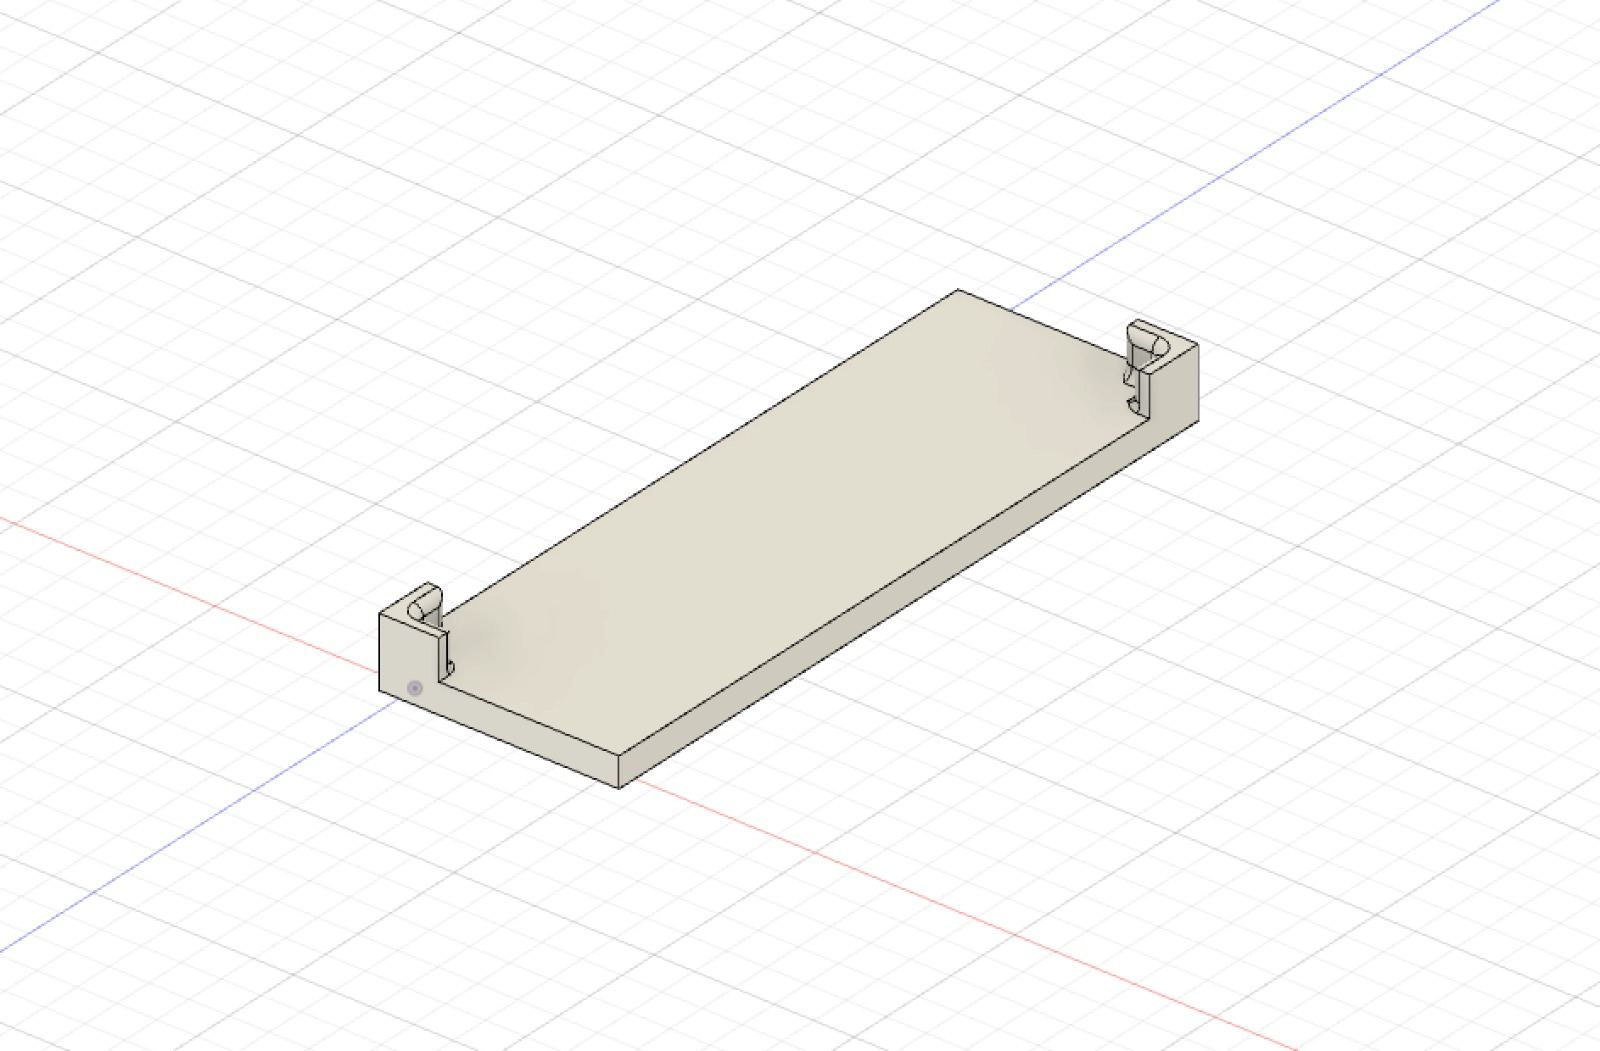
\includegraphics[scale = 0.2]{fig/Imagen_2_diseno_3D.jpeg}
\caption{Imagen 2 del diseño en 3D}
\label{fig:imagen-2-diseno-3d}
\end{figure}

\begin{figure}[tbp]
\centering
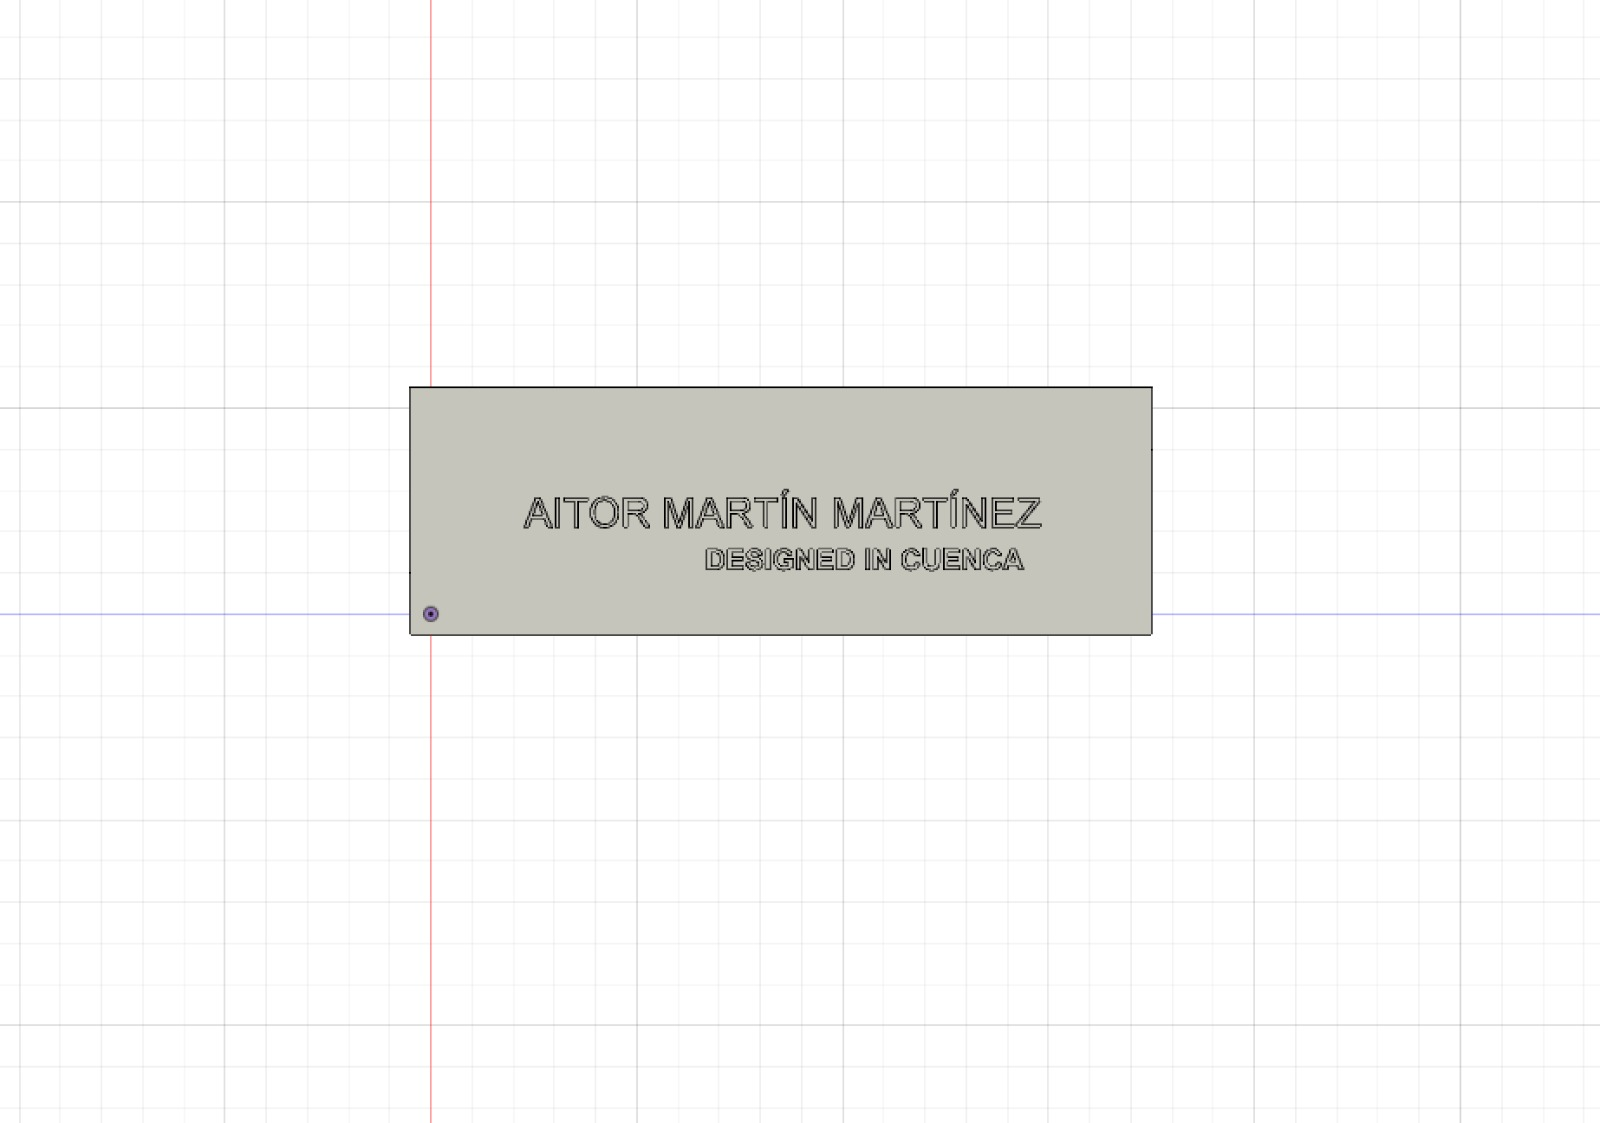
\includegraphics[scale = 0.2]{fig/Imagen_3_diseno_3D.jpeg}
\caption{Imagen 3 del diseño en 3D}
\label{fig:imagen-3-diseno-3d}
\end{figure}

\begin{figure}[tbp]
\centering
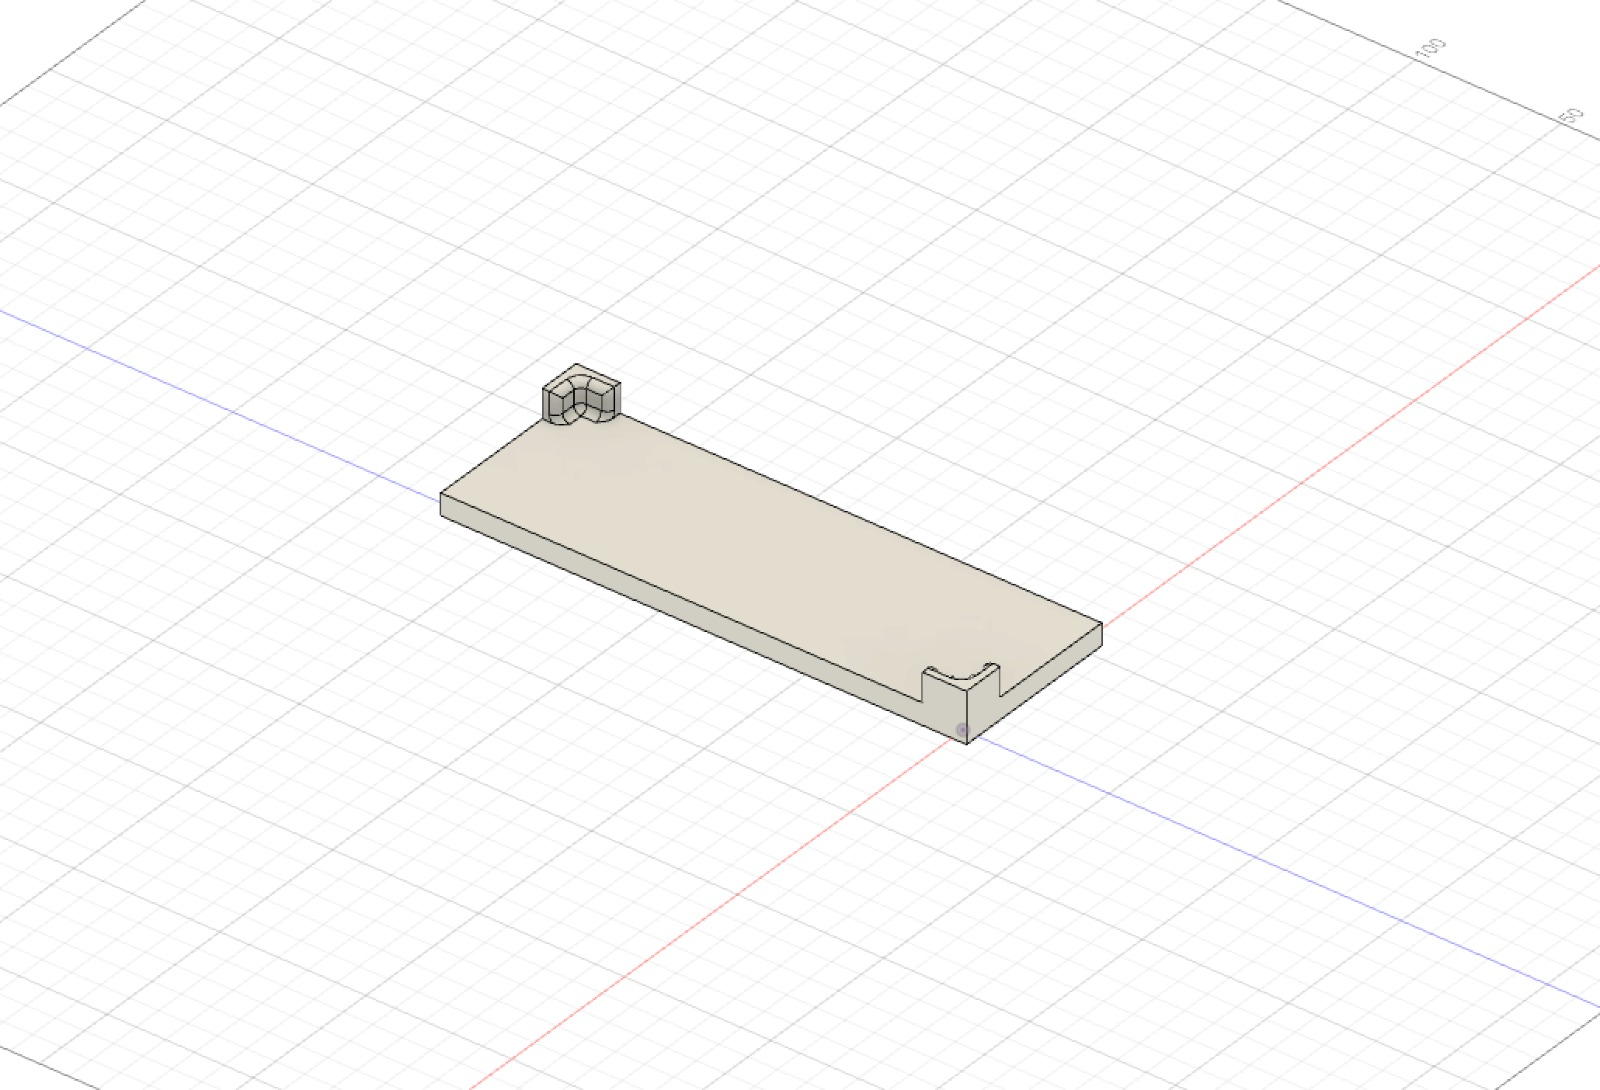
\includegraphics[scale = 0.2]{fig/Imagen_4_diseno_3D.jpeg}
\caption{Imagen 4 del diseño en 3D}
\label{fig:imagen-4-diseno-3d}
\end{figure}

\begin{figure}[tbp]
\centering
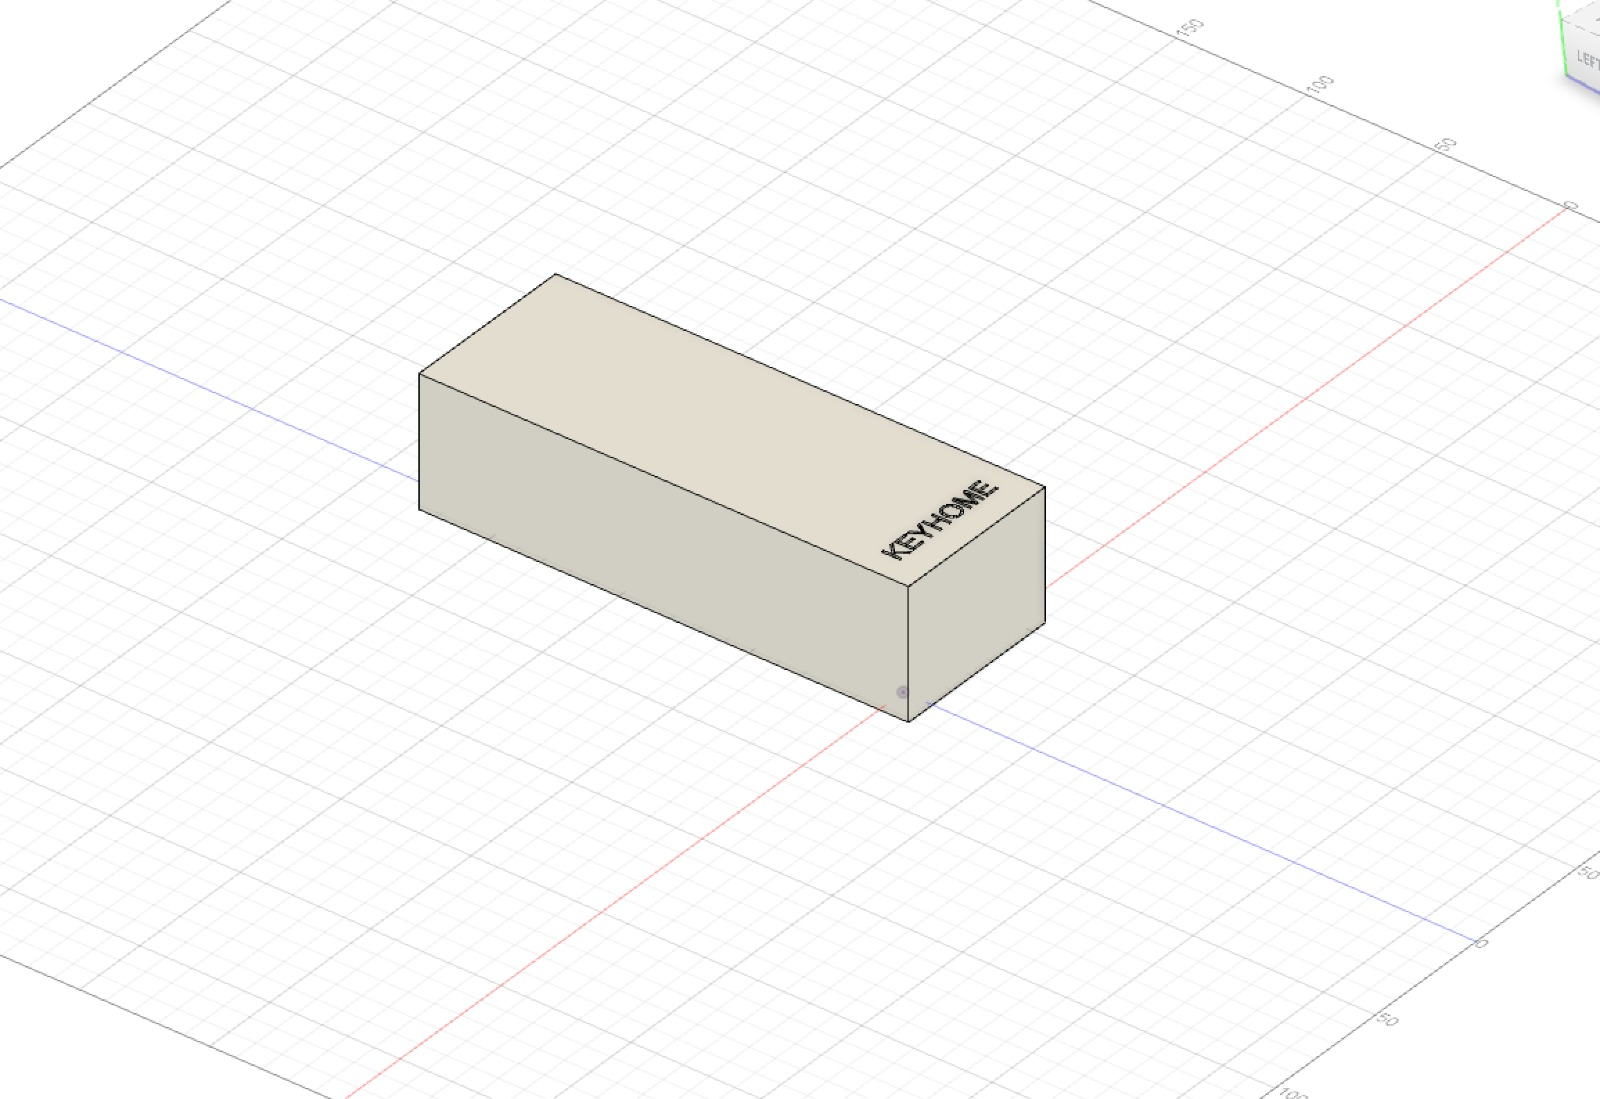
\includegraphics[scale = 0.2]{fig/Imagen_5_diseno_3D.jpeg}
\caption{Imagen 5 del diseño en 3D}
\label{fig:imagen-5-diseno-3d}
\end{figure}

Para que el proyecto funcione de forma correcta, este prototipo que contiene el circuito electrónico en su interior, deberá ser conducido hacia las conexiones realizadas en el portero automático que fueron explicadas en el primer apartado de este capitulo. Para conectar el interior del prototipo con el exterior, se hará uso de unos micro insertos roscados, que tienen un coste muy bajo y permiten incorporar estas conexiones de forma posterior a la impresión del prototipo.

Prestando atención a la figura~\ref{fig:imagen-2-diseno-3d}, puede observarse como la base de este dispositivo cuenta con dos esquinas ligeramente levantadas respecto al nivel del resto de la base. Con el fin de evitar, en la medida de lo posible, que intrusos abran el dispositivo, estos puntos serán perforados, junto con la tapa, por medio de un taladro que permitirá anclar un candado y cerrar de forma segura el dispositivo final. En la figura~\ref{fig:imagen-5-diseno-3d} se observa el aspecto visual que tendrá este dispositivo, una vez instalado en la vivienda.
\fi

\if00
\chapter{Resultados}
\label{ch:resultados}

La propia estructuración de los objetivos definidos para este trabajo de fin de grado servirá como base para la exposición de los resultados. De esta manera, se obtendrá un enfoque global, y a la vez, detallado, de cada una de las partes que componen el proyecto.

Para ello, al igual que en puntos anteriores, esta sección se dividirá en tres partes bien diferenciadas: Desarrollo del circuito electrónico, diseño de algoritmos y programación y tareas orientadas a la seguridad del dispositivo.
\section{Construcción del circuito electrónico}

La construcción del circuito electrónico definida en la fase de planificación contaba con dos objetivos principales, que eran los de realizar las conexiones necesarias para el correcto funcionamiento del dispositivo y fijar los elementos de manera segura y firme.

\begin{figure}[tbp]
\centering
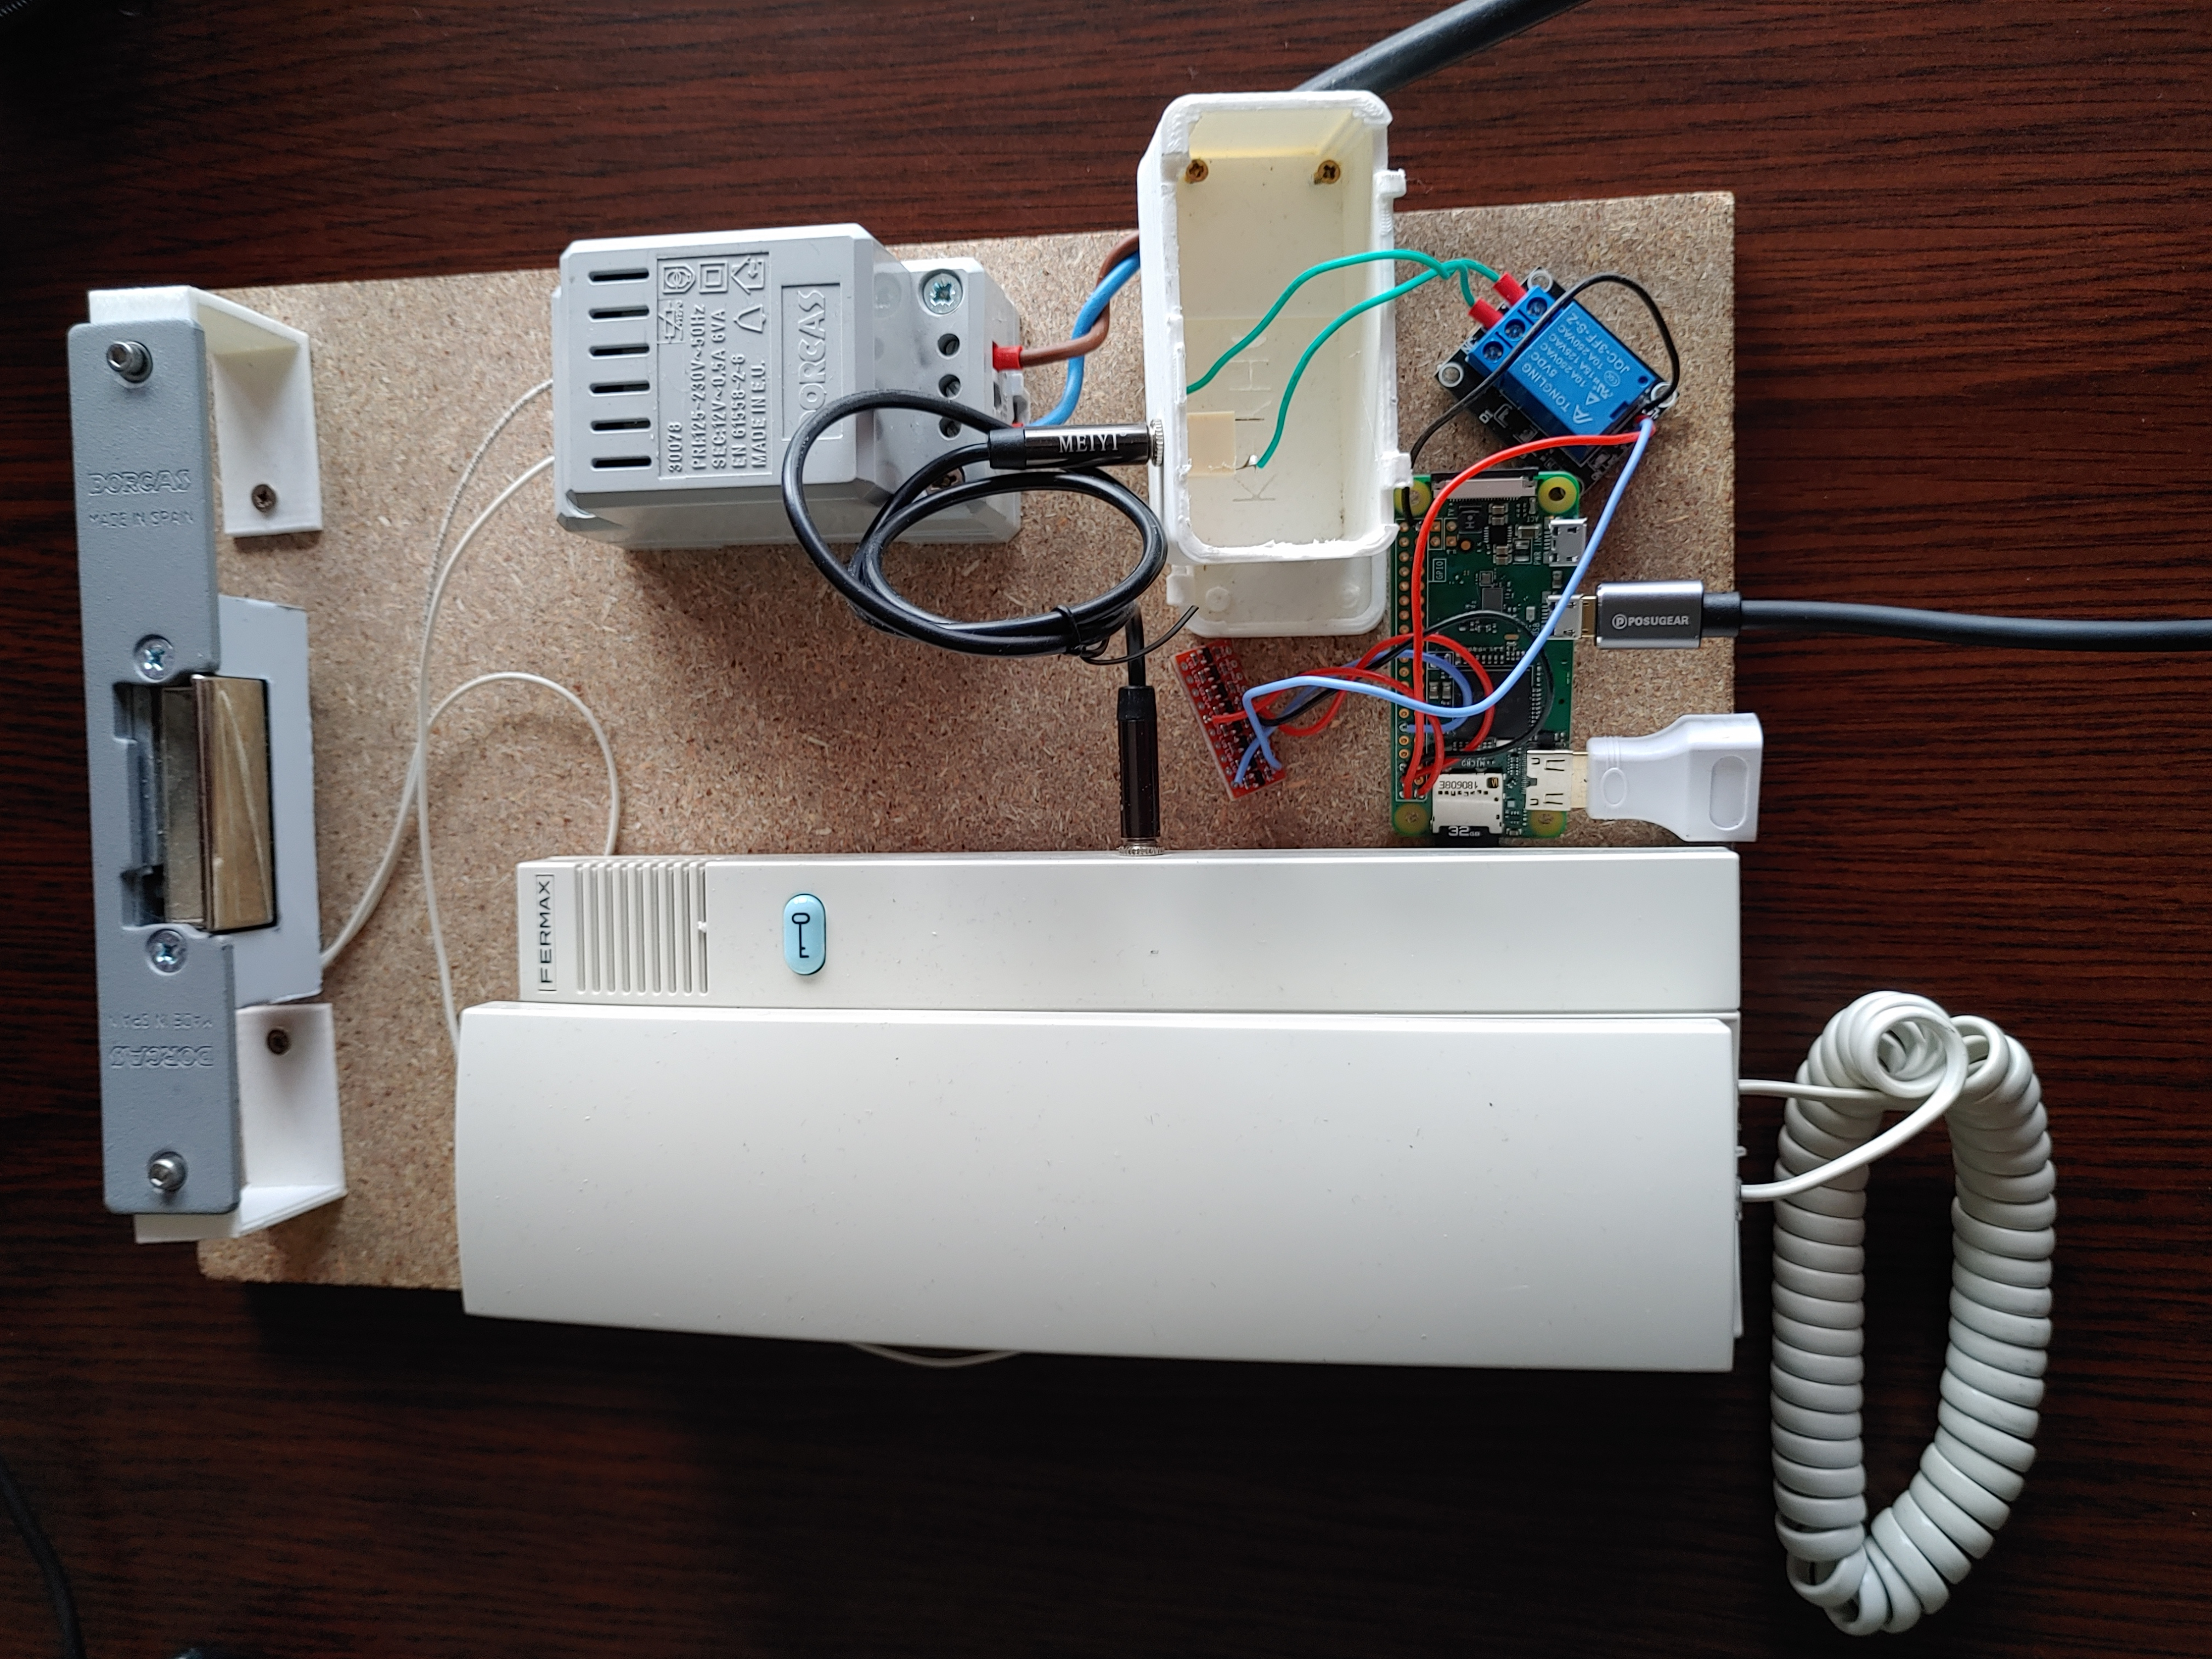
\includegraphics[scale = 0.1]{Prototipo_Completo.jpg}
\caption{Prototipo completo con todas las conexiones}
\label{fig:prototipo-completo}
\end{figure}
\begin{figure}[tbp]
\centering
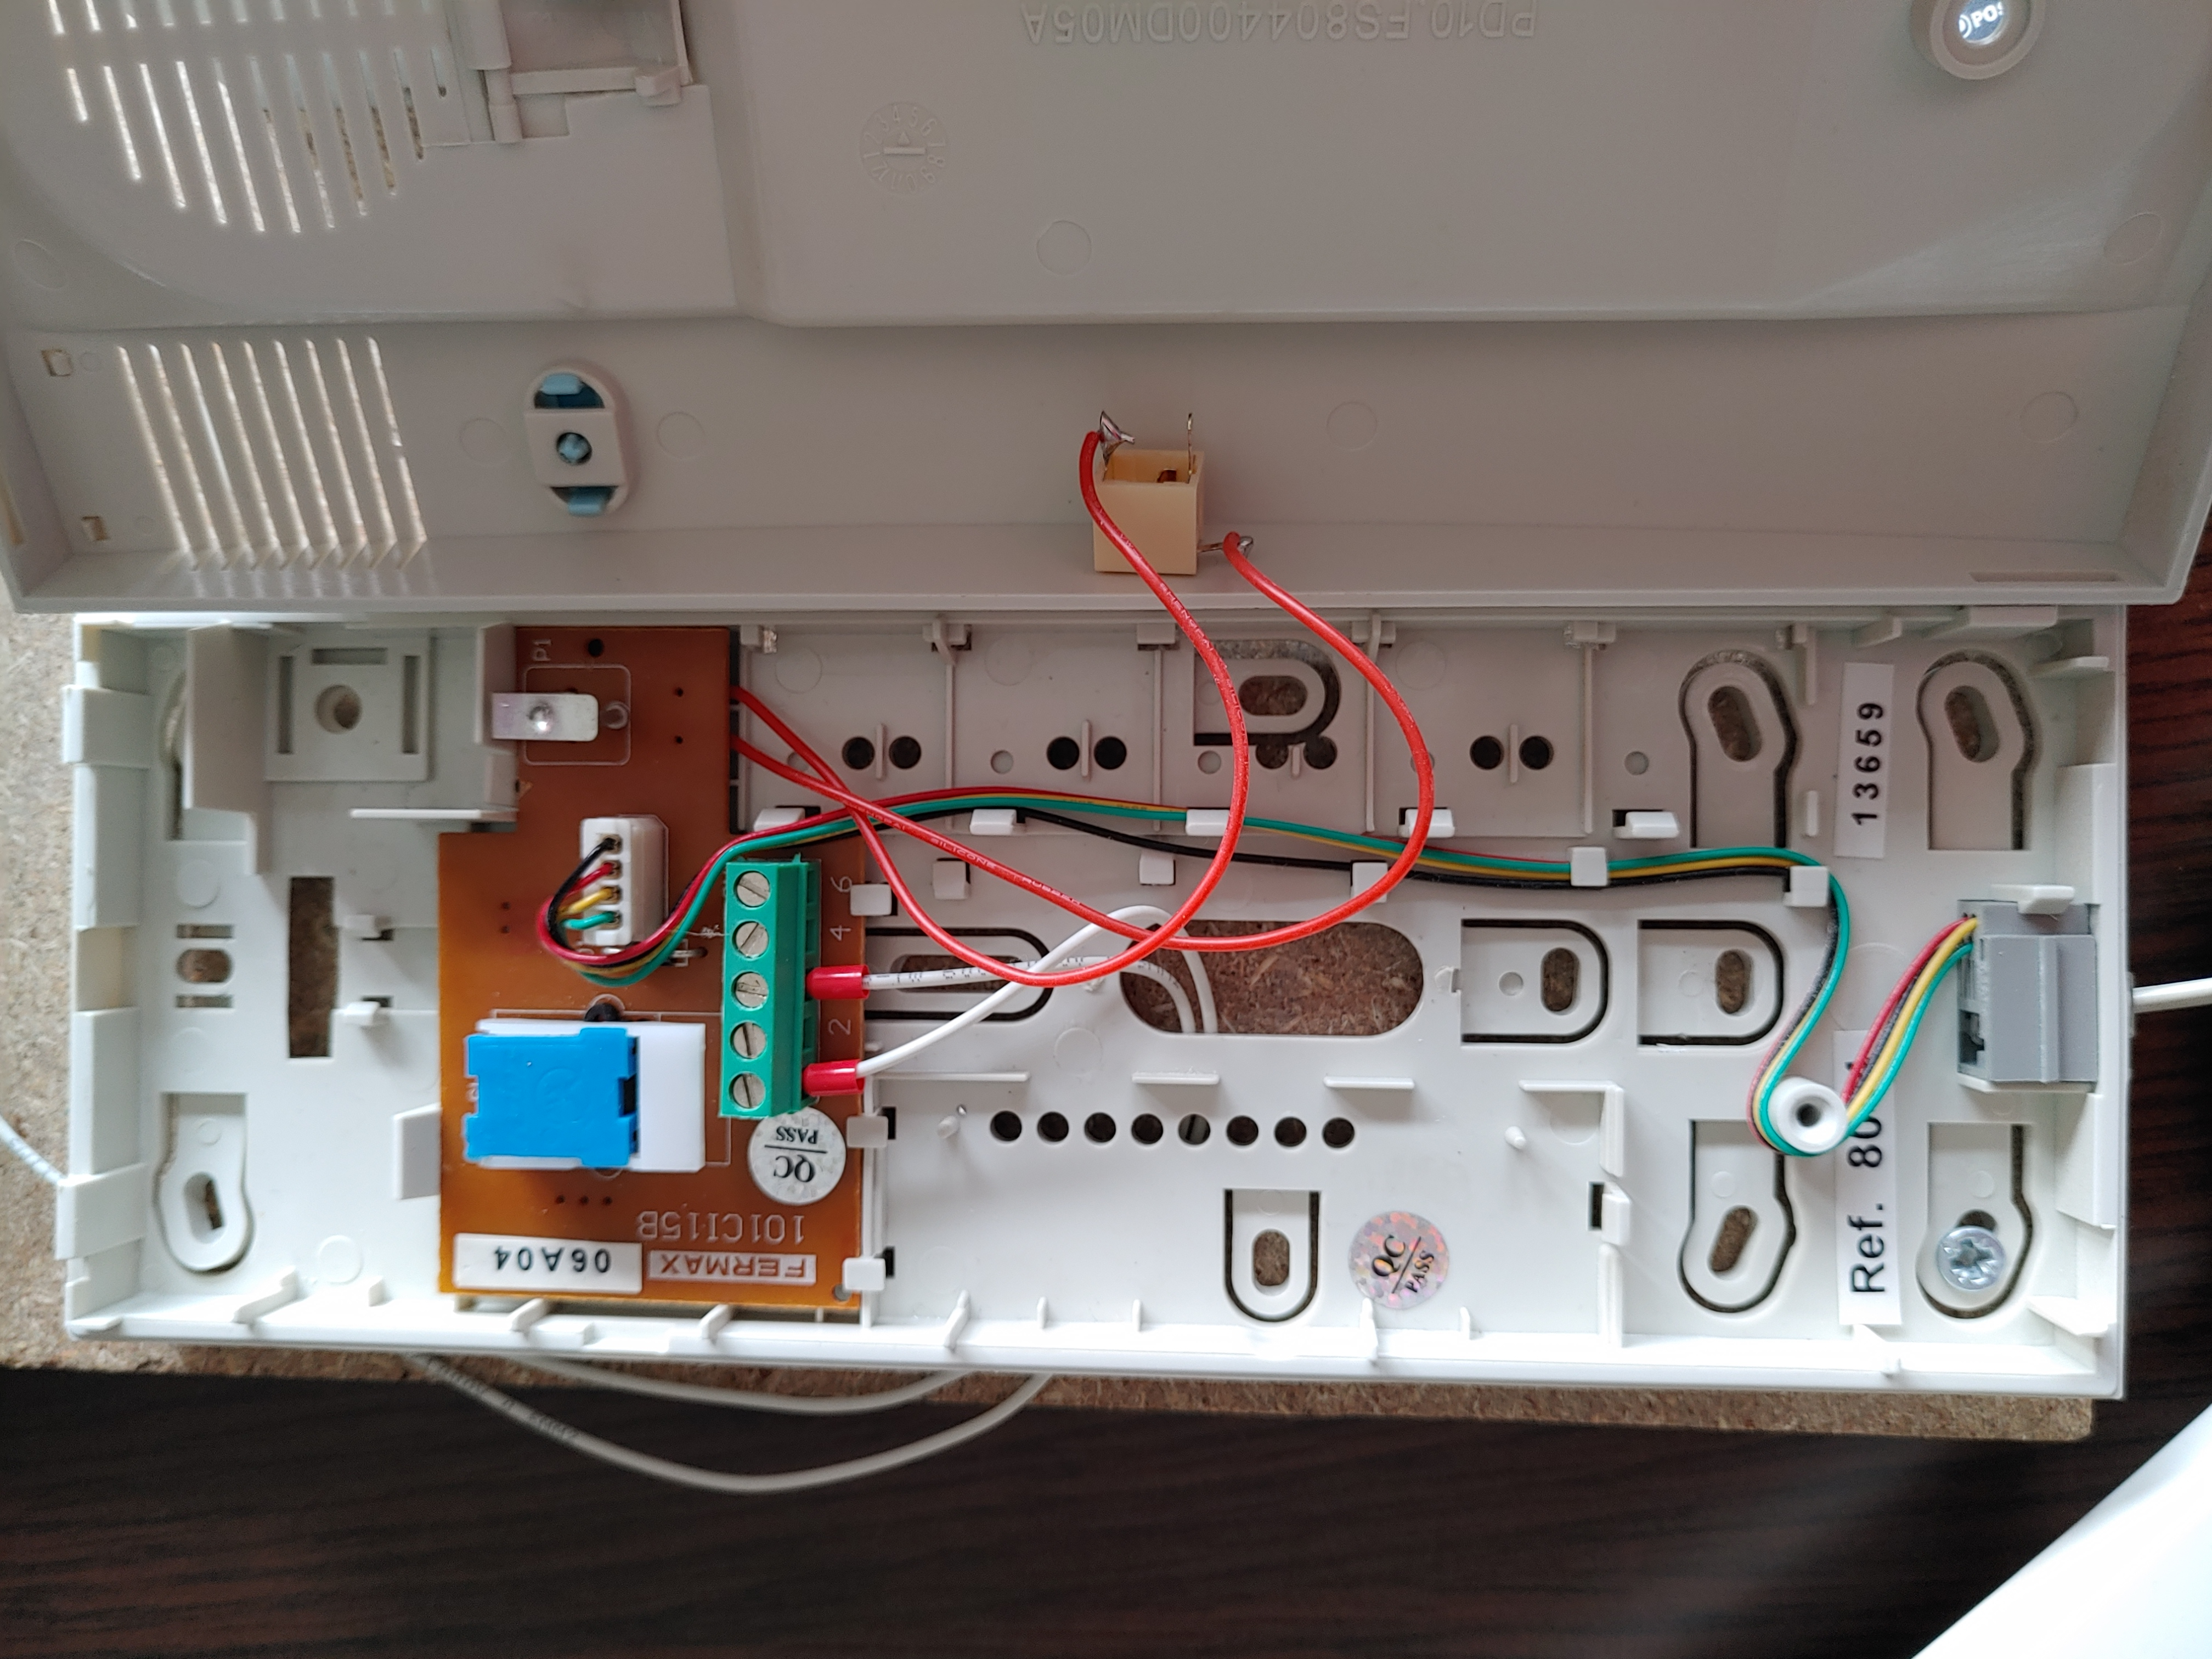
\includegraphics[scale = 0.1]{Interior_Portero_Automatico.jpg}
\caption{Conexiones en el interior del portero automático}
\label{fig:interior-portero-automatico}
\end{figure}

En las figura~\ref{fig:prototipo-completo} y ~\ref{fig:interior-portero-automatico} se puede observar el prototipo con todos los elementos que lo forman interconectados entre sí, tal como se definió en la fase de desarrollo. Tanto el portero automático, como la cerradura eléctrica y el transformador, han sido fijados por medio de tornillería a un tablón de madera que permite realizar, de forma segura y compacta, el transporte del prototipo.

Junto a estos elementos, puede observarse la interconexión de la Raspberry Pi Zero W con el conversor de nivel lógicos y el relé, que permiten el correcto funcionamiento de este prototipo.

La interconexión que adapta el sistema con el portero automático se ha hecho por medio de un conector tipo mini jack, con la intención de hacer que sea más intuitivo para el usuario final.

Queda expuesto por tanto, de forma gráfica, como los dos puntos principales que quedaron definidos para esta fase inicial han sido cumplidos de forma exitosa.

\section{Diseño de algoritmos y programación}
En el apartado de planificación del presente trabajo queda constancia de las diferentes materias que debían tenerse en cuenta en lo referente al diseño de algoritmos y programación.

\subsection{Programa capaz de activar la cerradura en los momentos precisos}

La primera característica que se implementa en el proyecto es la de hacer un programa capaz de activar una señal que permita realizar la apertura de la cerradura, ayudándose para ello del circuito construido previamente. Este programa debía poder estar controlado por un administrador que contara con la posibilidad de crear y anular reservas, realizar la apertura de la puerta y dejar las tareas de administración.

Una vez realizada la integración de los códigos implementados en la fase de desarrollo, y ejecutados por medio de la Raspberry Pi, se obtienen los resultados esperados, dando lugar a un panel de administración como el que se observa en la figura~\ref{fig:panel-de-administrador}.
\begin{figure}[tbp]
\centering
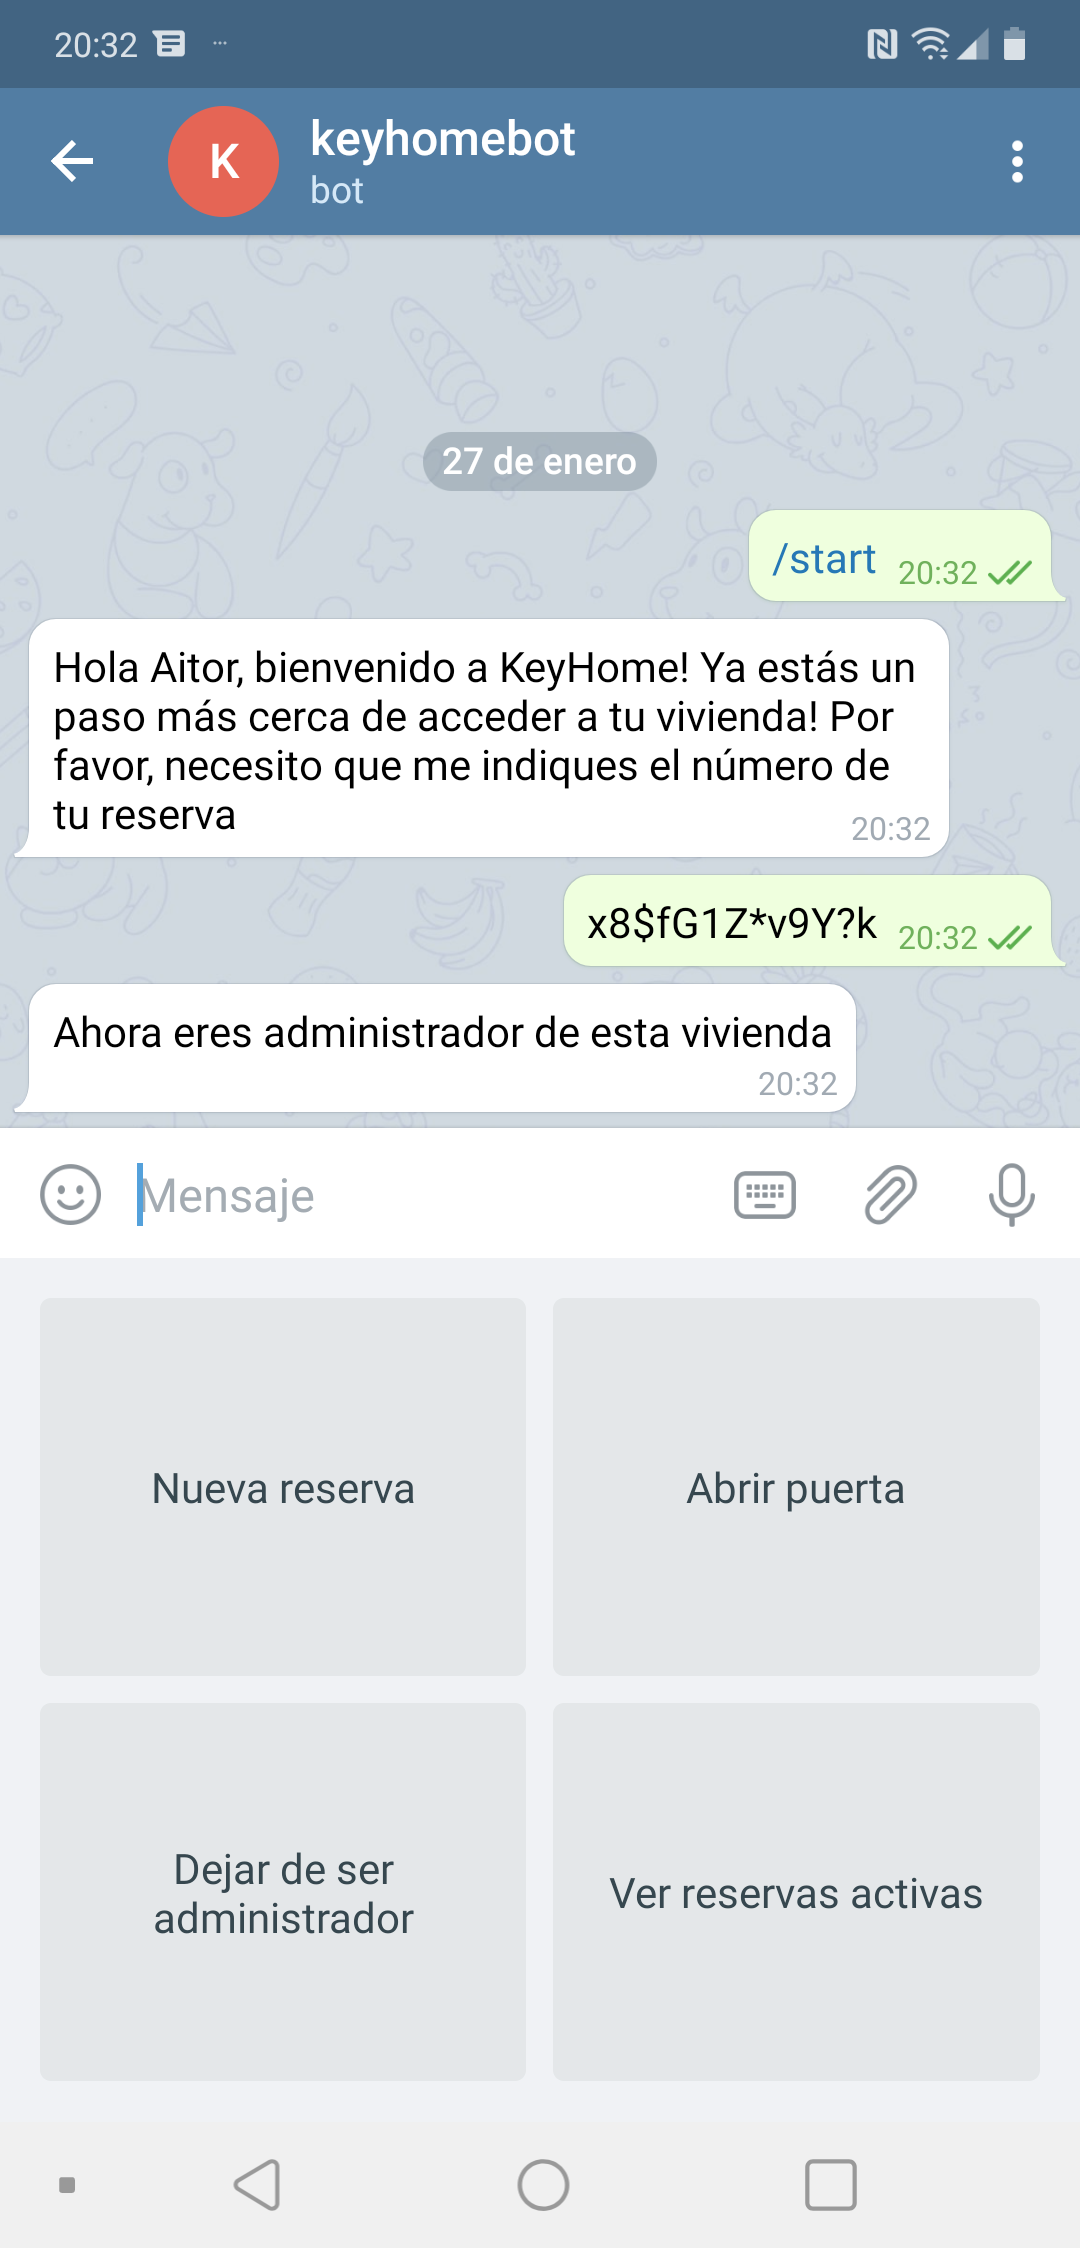
\includegraphics[scale = 0.15]{fig/Panel_de_administrador.png}
\caption{Panel de administrador}
\label{fig:panel-de-administrador}
\end{figure}

\subsubsection{Creación de nuevas reservas}

Entre las tareas de este apartado, destacan aquellas que tienen por objeto automatizar la entrada de nuevas reservas en el sistema. Sin embargo, por diferentes razones, es recomendable incluir la posibilidad al administrador de que él mismo pueda añadir estas reservas. Para ello, en la figura~\ref{fig:panel-de-administrador} se puede observar como se ha creado un apartado de crear reservas. Si hacemos uso de esta opción, el bot pedirá, en primer lugar, que se indique el número de reserva, tal como se puede observar en la figura~\ref{fig:introduccion-del-numero-de-reserva}. Este número de reserva será aquel con el que el huésped podrá acceder a la vivienda el día en que comience su estancia.
\begin{figure}[tbp]
\centering
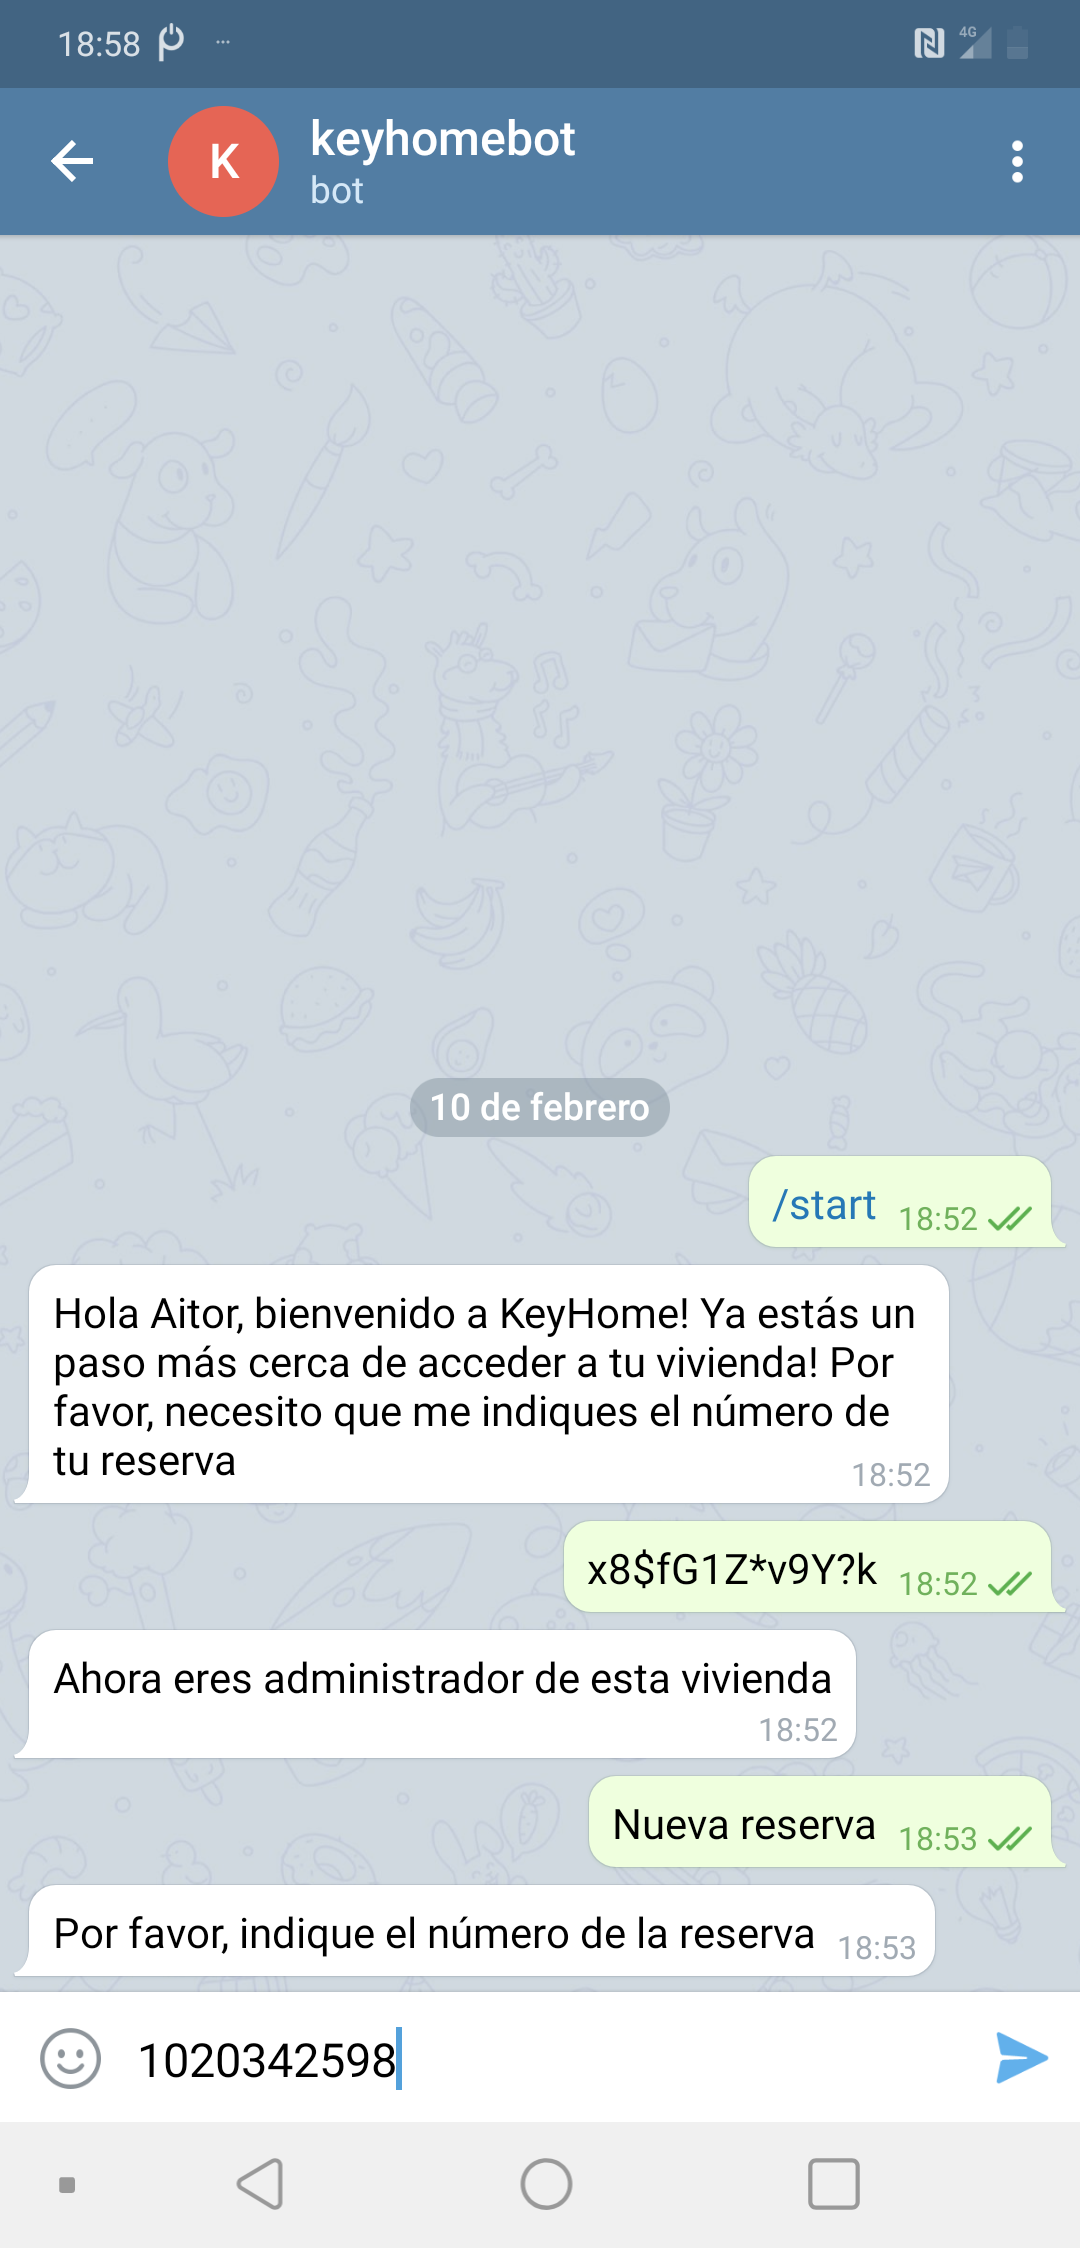
\includegraphics[scale = 0.15]{fig/Numero-de-reserva.png}
\caption{Introducción del número de reserva}
\label{fig:introduccion-del-numero-de-reserva}
\end{figure}

Una vez que el administrador introduzca el número de reserva, lo siguiente que le es exigido por parte del bot son las fechas de entrada y de salida del cliente, tal como puede observarse en la figura~\ref{fig:introduccion-de-las-fechas-de-reserva}, donde se establecen las fechas en las que el cliente podrá acceder a la vivienda.

\begin{figure}[tbp]
\centering
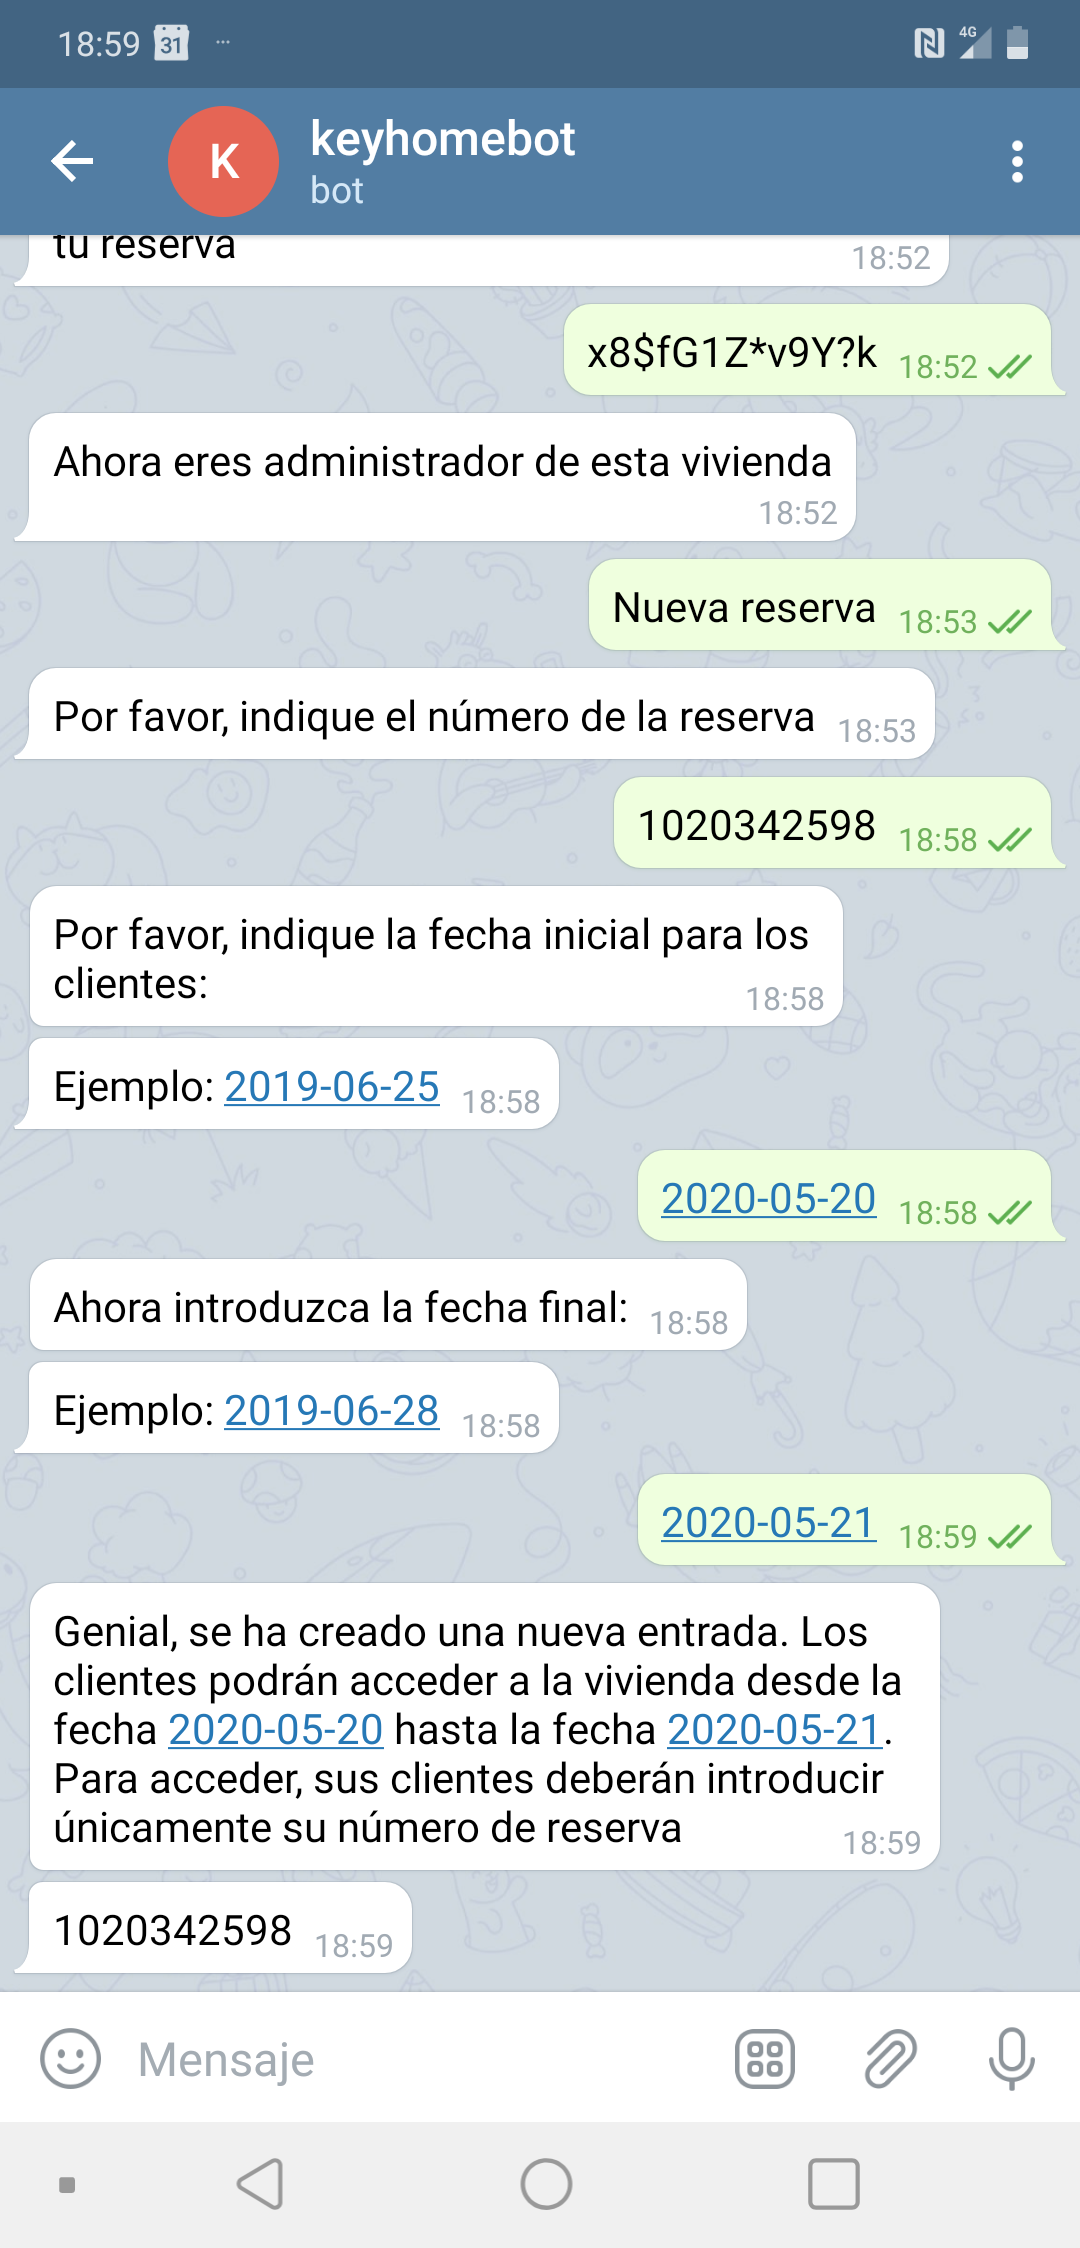
\includegraphics[scale = 0.15]{fig/Fechas-de-reserva.png}
\caption{Introducción de las fechas de reserva}
\label{fig:introduccion-de-las-fechas-de-reserva}
\end{figure}

\subsubsection{Apertura de la cerradura por parte del administrador}

La siguiente función que debe cumplirse, siguiendo la programación de las tareas, sería la de permitir que el administrador de la vivienda tuviese la posibilidad de abrir la puerta. Esta posibilidad queda habilitada en el programa central definido en el apartado de desarrollo de este documento, a través del cual se crea el resultado que se muestra en la figura~\ref{fig:apertura-de-puerta-por-parte-del-administrador}, donde un administrador activa la apertura de la cerradura desde su panel de control.

\begin{figure}[tbp]
\centering
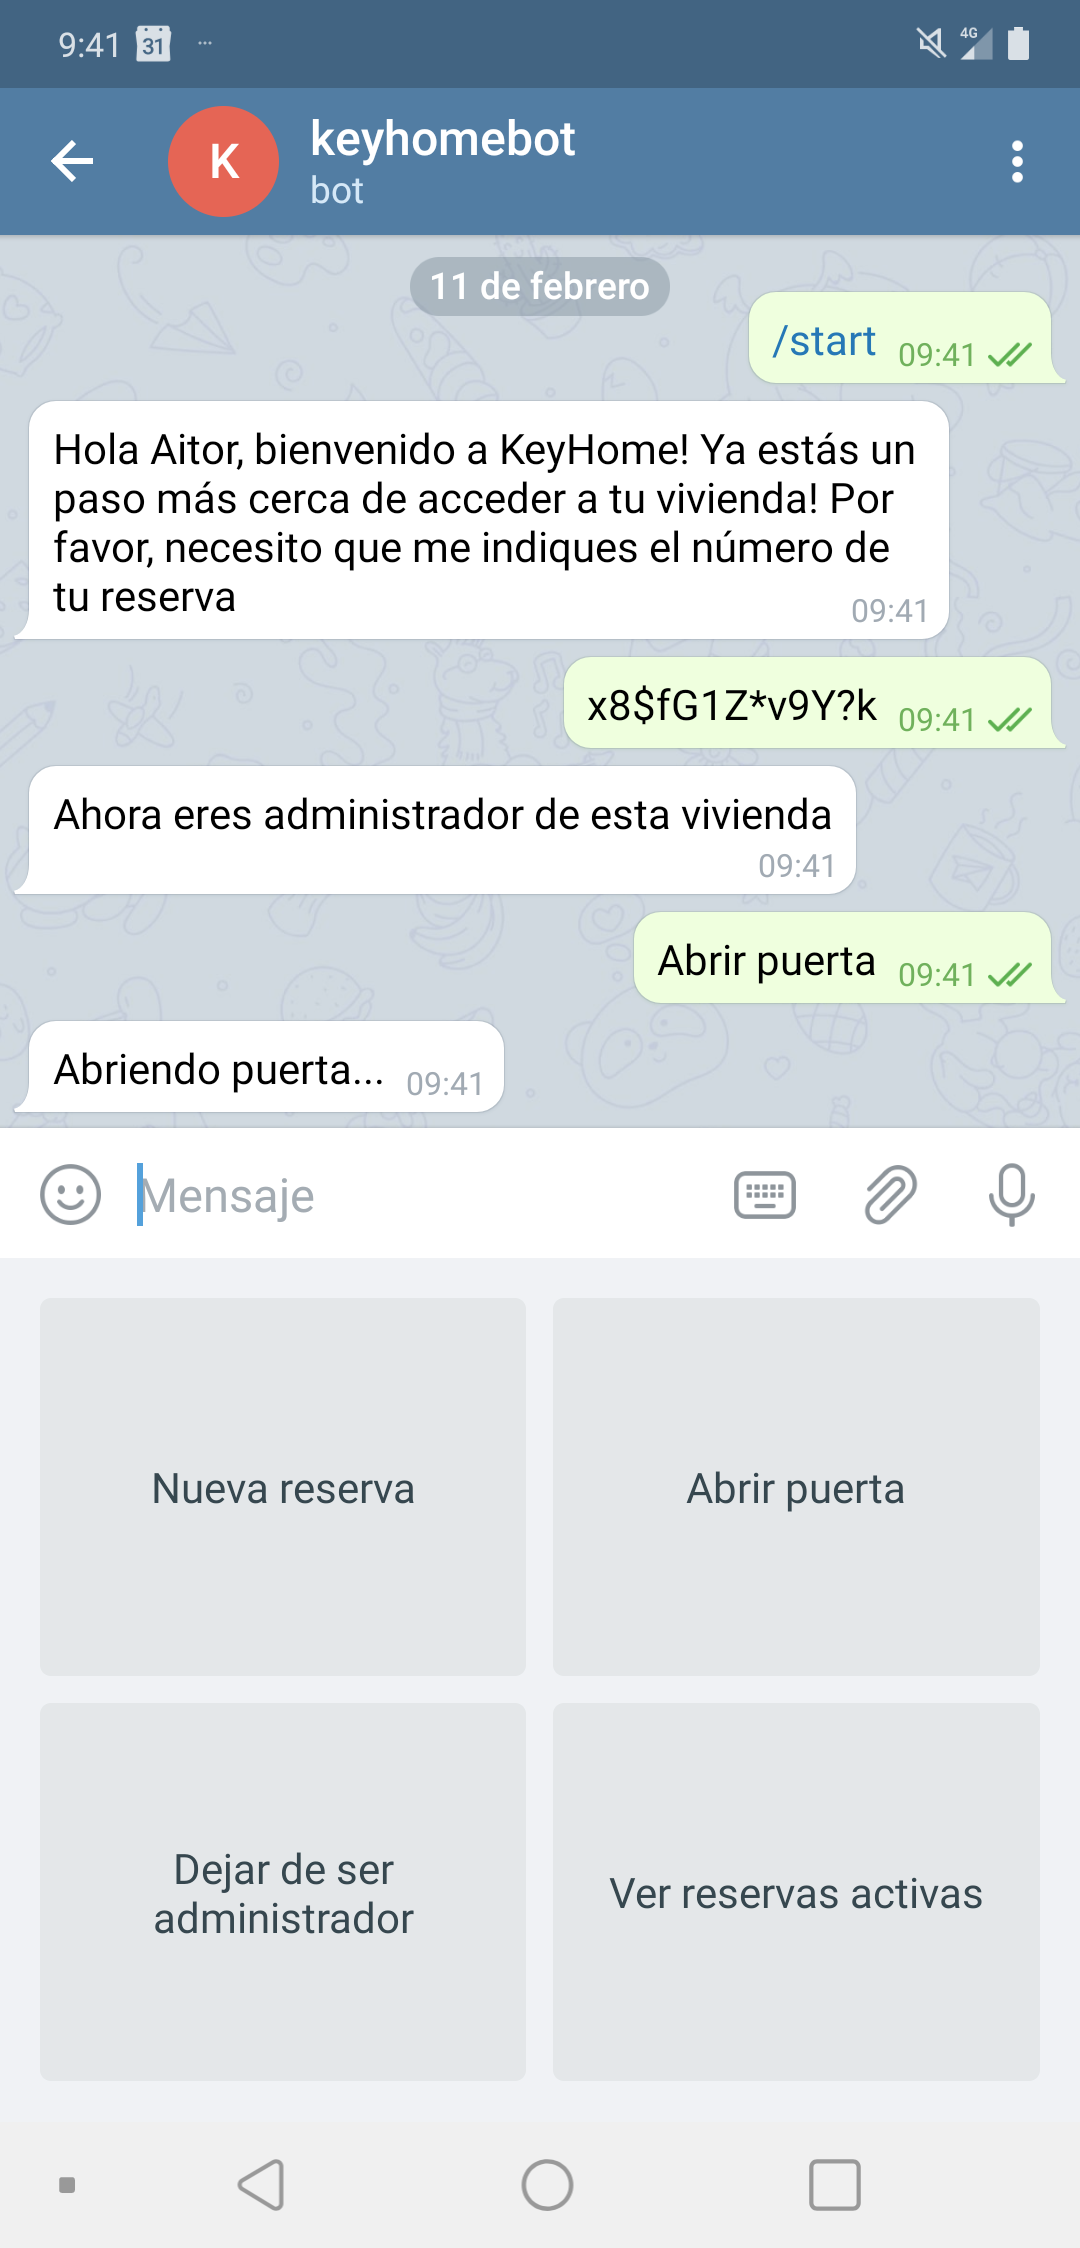
\includegraphics[scale=0.15]{fig/Apertura-de-puerta-administrador.png}
\caption{Apertura de puerta por parte del administrador}
\label{fig:apertura-de-puerta-por-parte-del-administrador}
\end{figure}

\subsubsection{Dejar permisos de administrador}

Por diferentes razones, se puede dar la situación de que una persona que ha sido administradora de la vivienda durante un tiempo, no deba continuar ejerciendo como tal. Para ello, se decidió habilitar esta aplicación con la posibilidad de dejar ese cargo, tal como puede observarse en la figura~\ref{fig:administrador-dejando-sus-permisos-de-administracion}, donde un administrador deja los permisos como administrador.

\begin{figure}[tbp]
\centering
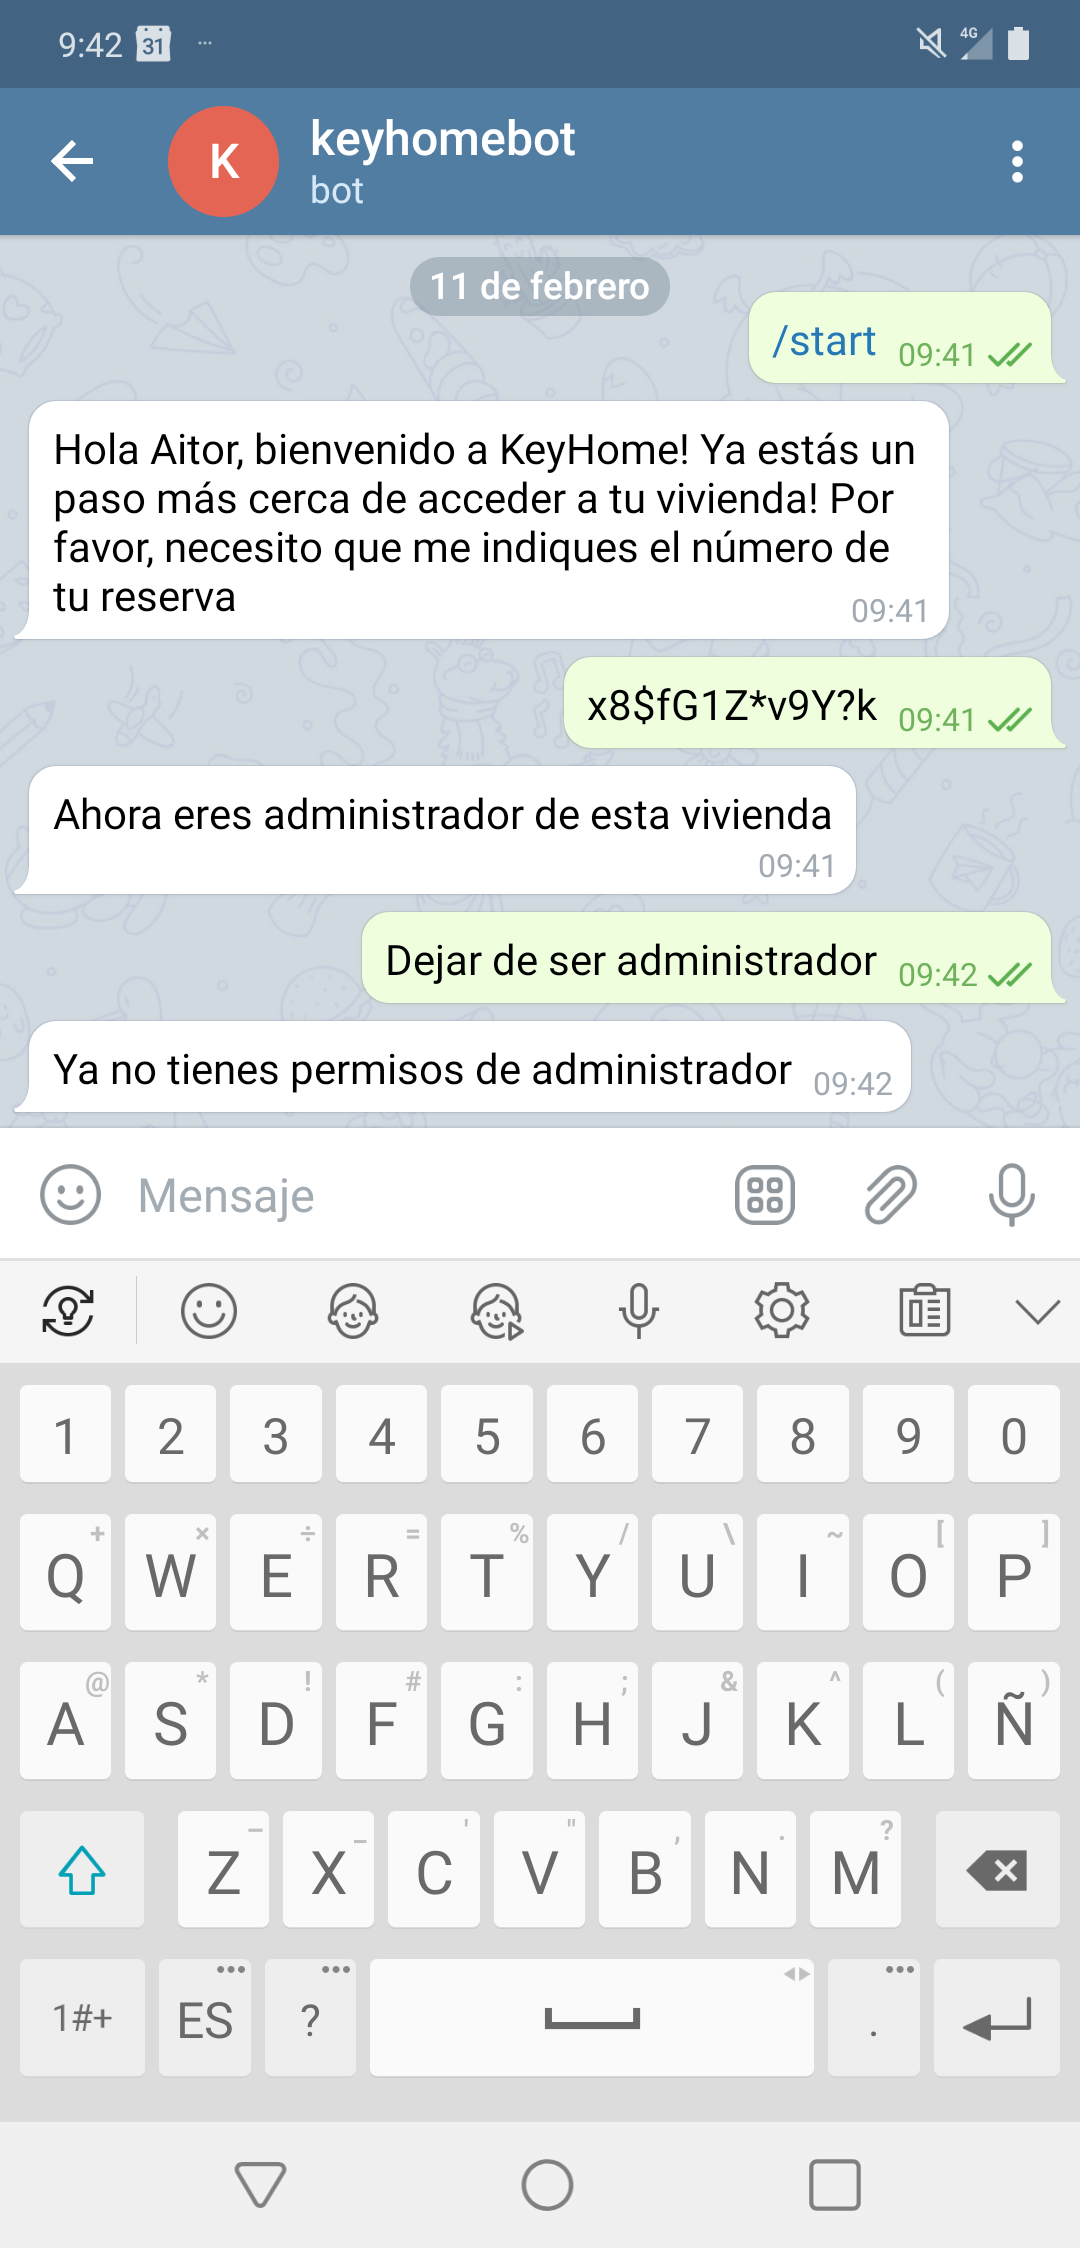
\includegraphics[scale=0.15]{fig/Dejar-de-ser-administrador.png}
\caption{Administrador dejando sus permisos de administración}
\label{fig:administrador-dejando-sus-permisos-de-administracion}
\end{figure}

\subsubsection{Consulta y modificación de reservas}

El último punto que se determinó añadir a los poderes de administrador, fue el de incluir la posibilidad de consultar las reservas, y además, poder anular aquellas que se considere. Es en la figura~\ref{fig:consulta-y-moficicacion-de-reservas}, donde se observa como el administrador de la vivienda consulta las diferentes fechas que hay disponibles, eliminando una de ellas a modo de ejemplo.

\begin{figure}[tbp]
\centering
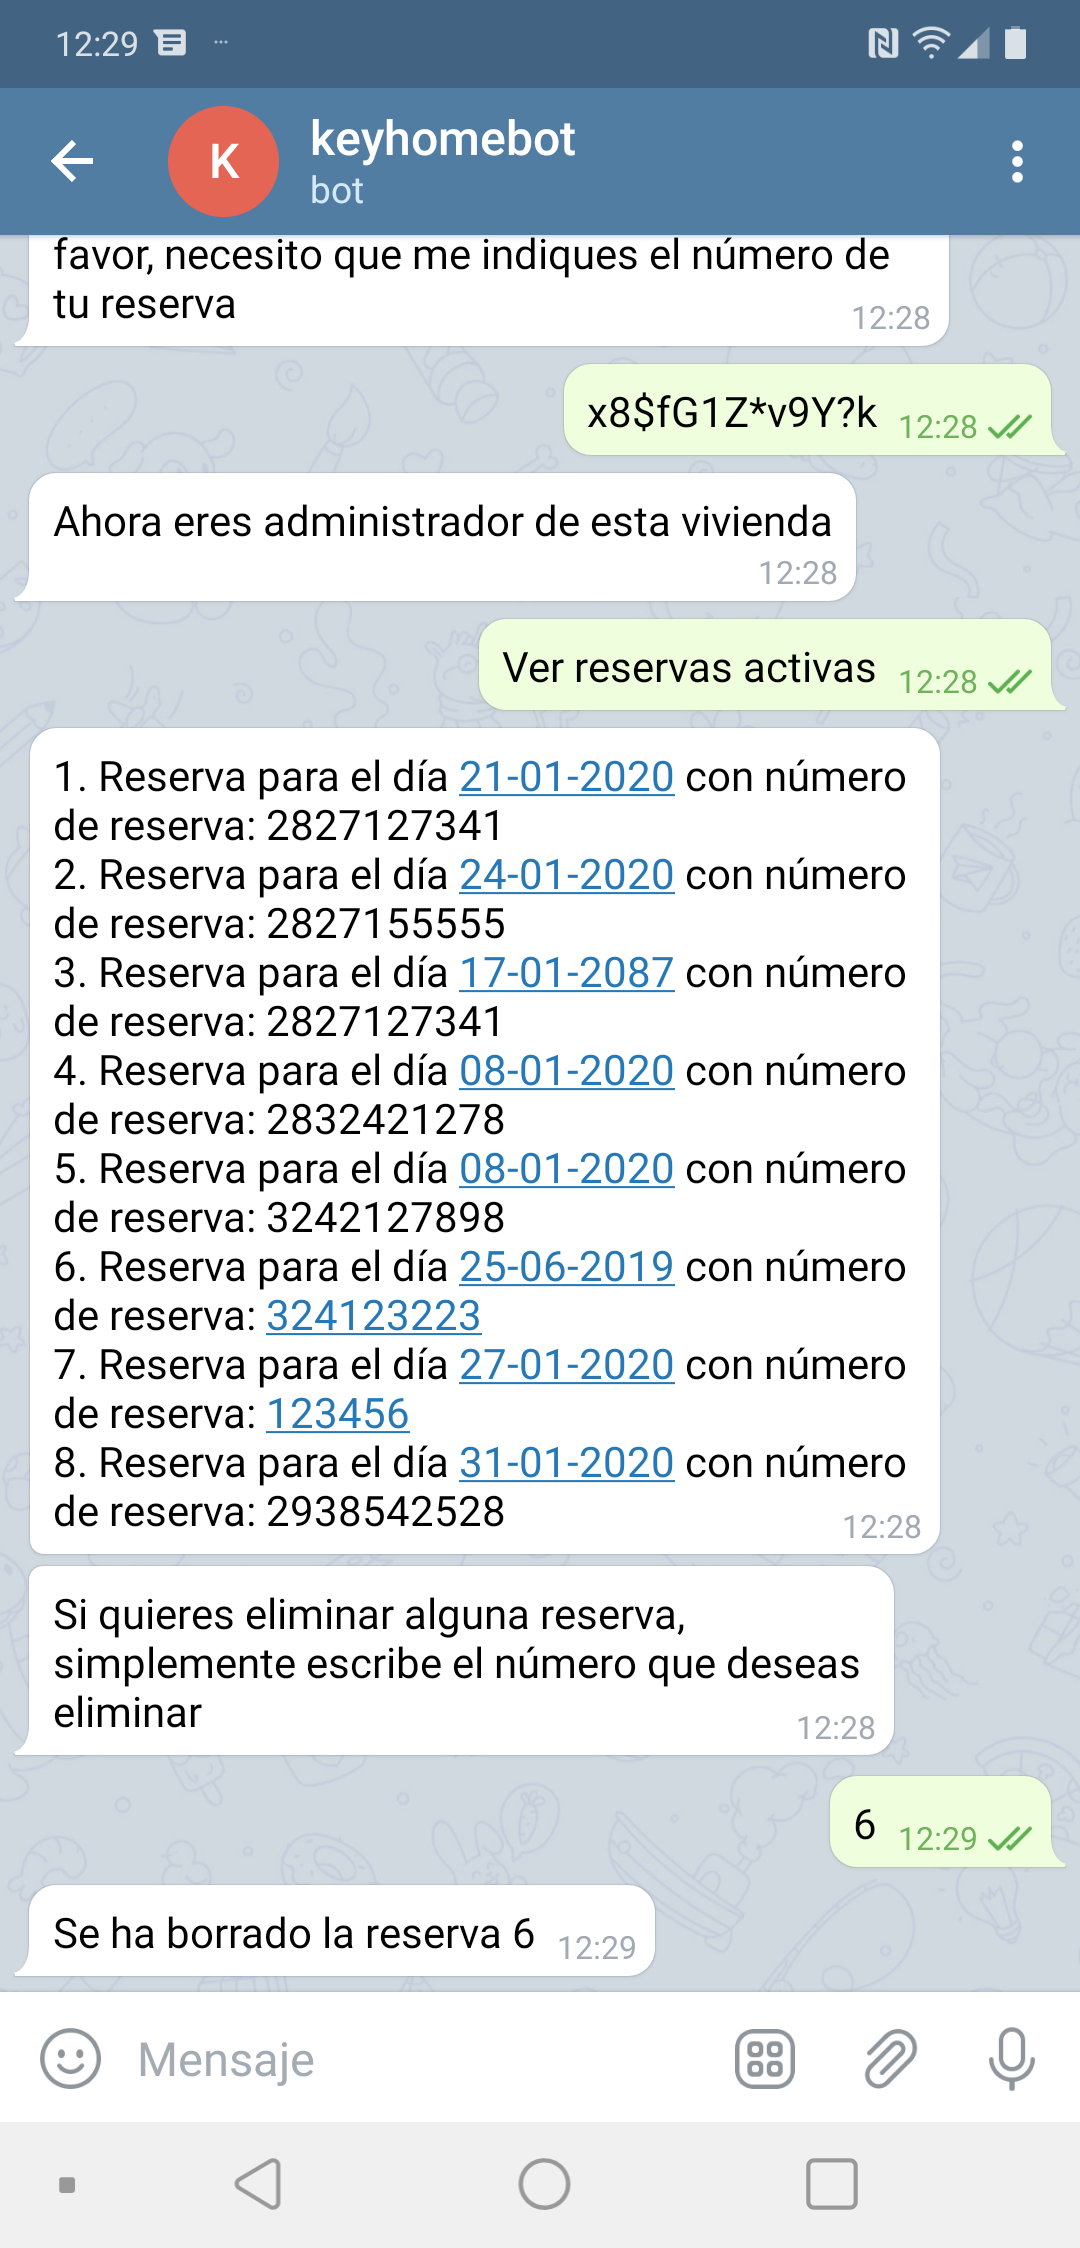
\includegraphics[scale=0.15]{fig/Consulta-y-modificacion-reservas.png}
\caption{Consulta y modificación de reservas}
\label{fig:consulta-y-moficicacion-de-reservas}
\end{figure}

A parte del administrador, la única figura que forma parte de este proyecto es la del usuario final o huésped de la vivienda, el cual debe tener a su disposición la posibilidad de abrir la puerta en el momento de su llegada. En la figura~\ref{fig:apertura-de-puerta-por-parte-del-huesped} puede observarse como este usuario final introduce su número de reserva, y al estar activo en ese momento, se le permite acceder a la vivienda realizando la apertura automática de la cerradura.

\begin{figure}[tbp]
\centering
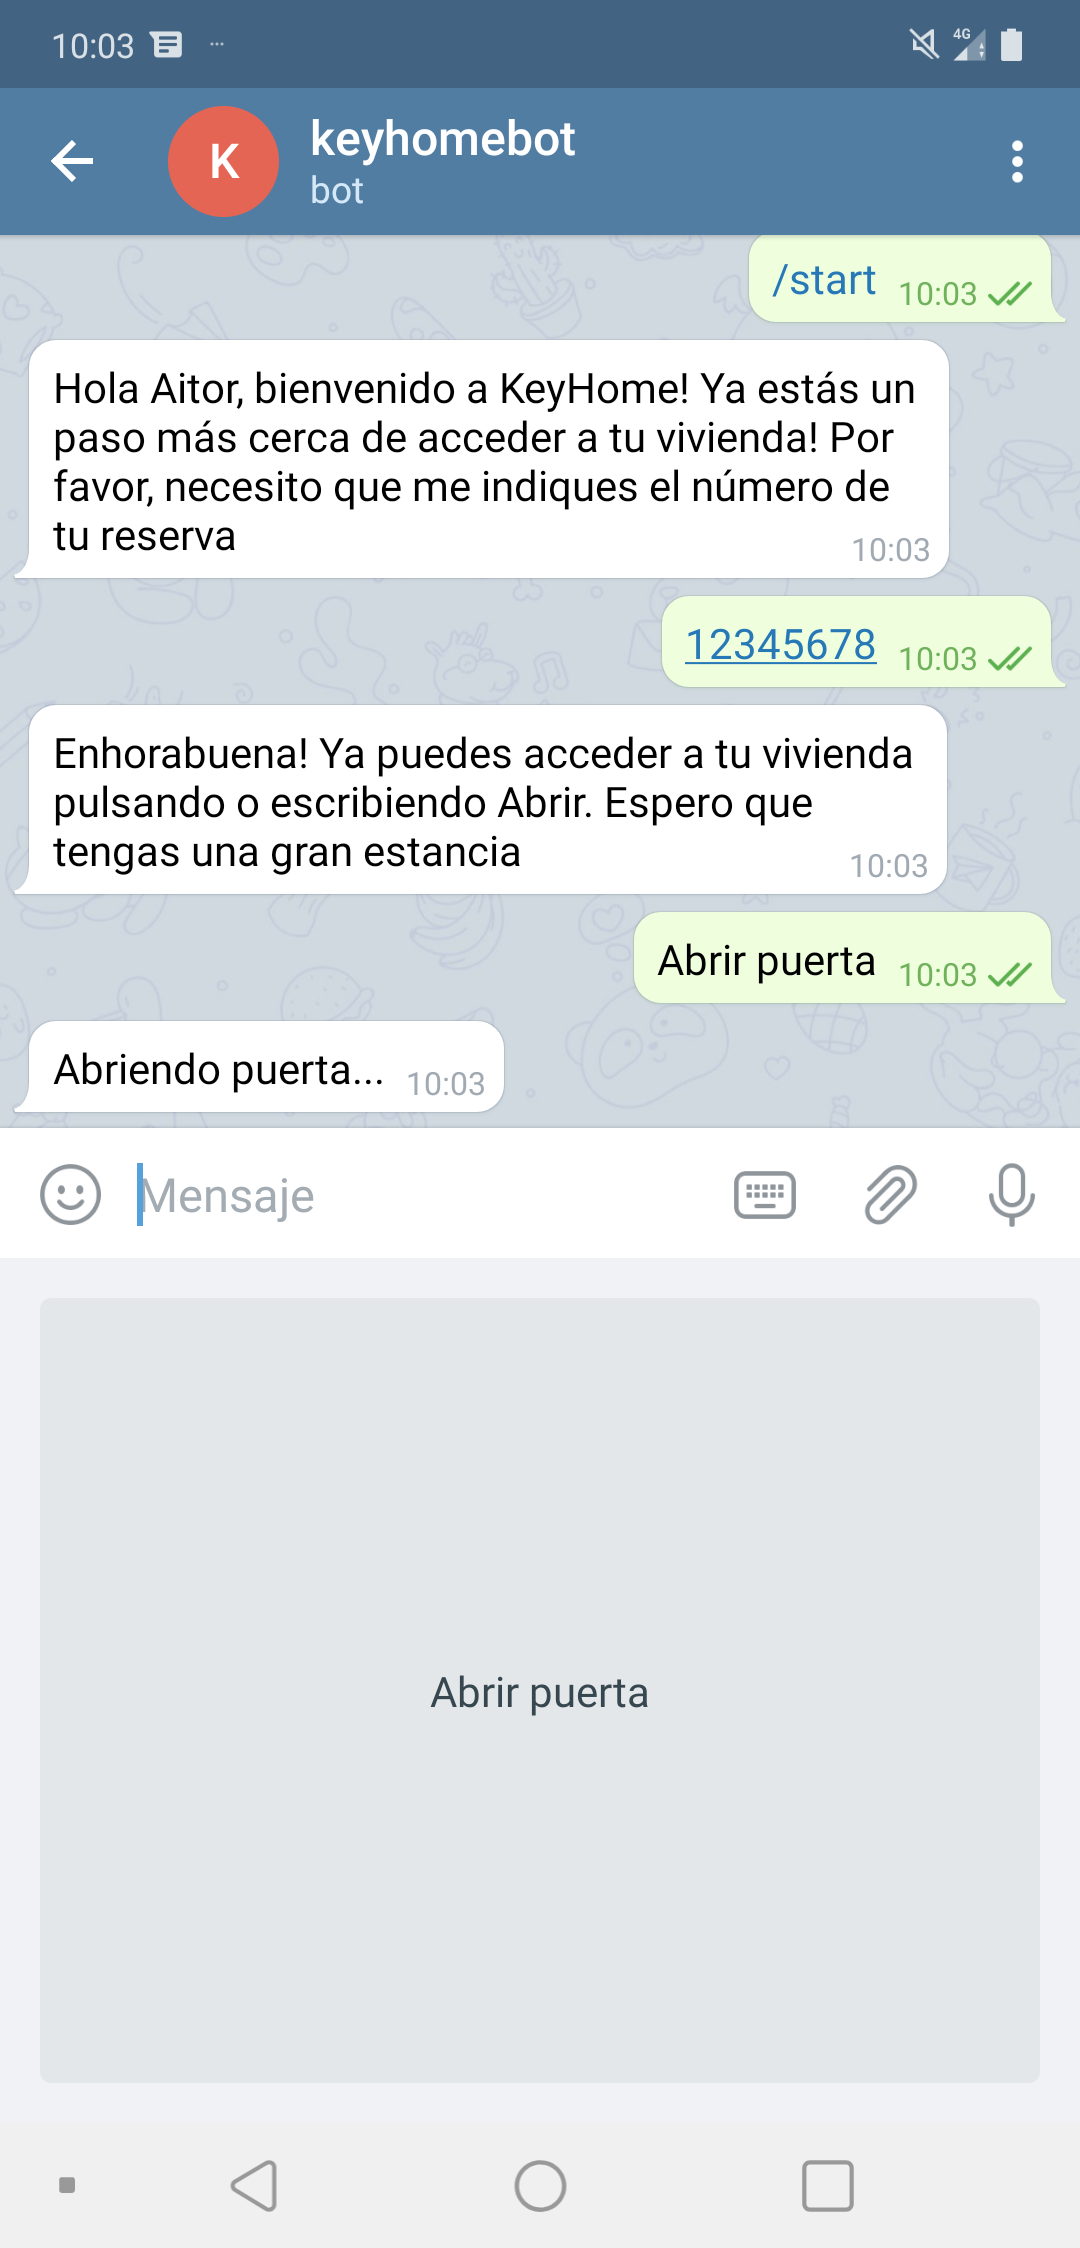
\includegraphics[scale=0.15]{fig/Apertura-de-puerta-por-parte-del-huesped.png}
\caption{Apertura de la cerradura por parte del huésped}
\label{fig:apertura-de-puerta-por-parte-del-huesped}
\end{figure}

\subsubsection{Automatización de la entrada y cancelación de reservas}

Existen muchas plataformas de alquiler vacacional. Para la elaboración de este sistema automático de recepción de reservas se ha hecho un programa, descrito en el apartado de desarrollo del presente documento, que automatiza las reservas de la plataforma Booking. Se ha tomado esta decisión, en base a dos razones principales:
\begin{enumerate}
\item Es la plataforma más utilizada en la actualidad.
\item Para la elaboración de este programa se ha podido utilizar el modelo de correo que envía Booking en la actualidad, con lo que la automatización descrita en este punto es completamente funcional.
\end{enumerate}

El resultado obtenido en este apartado ha sido el esperado, ya que ante una entrada de nueva reserva, notificada a la aplicación por medio de correo electrónico recibido de Booking, se ha conseguido incorporar dicha reserva en el historial de reservas que pueden ser consultados y modificados por el anfitrión. De igual manera, cuando Booking informa de una cancelación, por medio de un correo electrónico, este es recibido por el programa descrito en el apartado de desarrollo, el cual se encarga de eliminar dicha reserva del sistema incorporado en la Raspberry Pi, eliminando así toda posibilidad de acceso para el cliente que ha cancelado.

\subsection{Seguridad del dispositivo}
Al igual que en los puntos que preceden a este, la metodología de análisis de resultados consistirá en evaluar los frutos que han sido obtenidos del trabajo desempeñado en la fase de desarrollo.

El primer programa que se realizó consistía en un sistema de detección que avisara al propietario en caso de que alguien abriera la caja donde se encuentra el circuito.
El funcionamiento de este programa es correcto, actuando de manera que, en caso de que alguien abra la caja, el detector de distancia ofrecerá una medida mayor, y ante tal suceso, el programa enviará un correo electrónico como el que puede verse en la figura~\ref{fig:aviso-ante-posible-manipulacion}.

\begin{figure}[tbp]
\centering
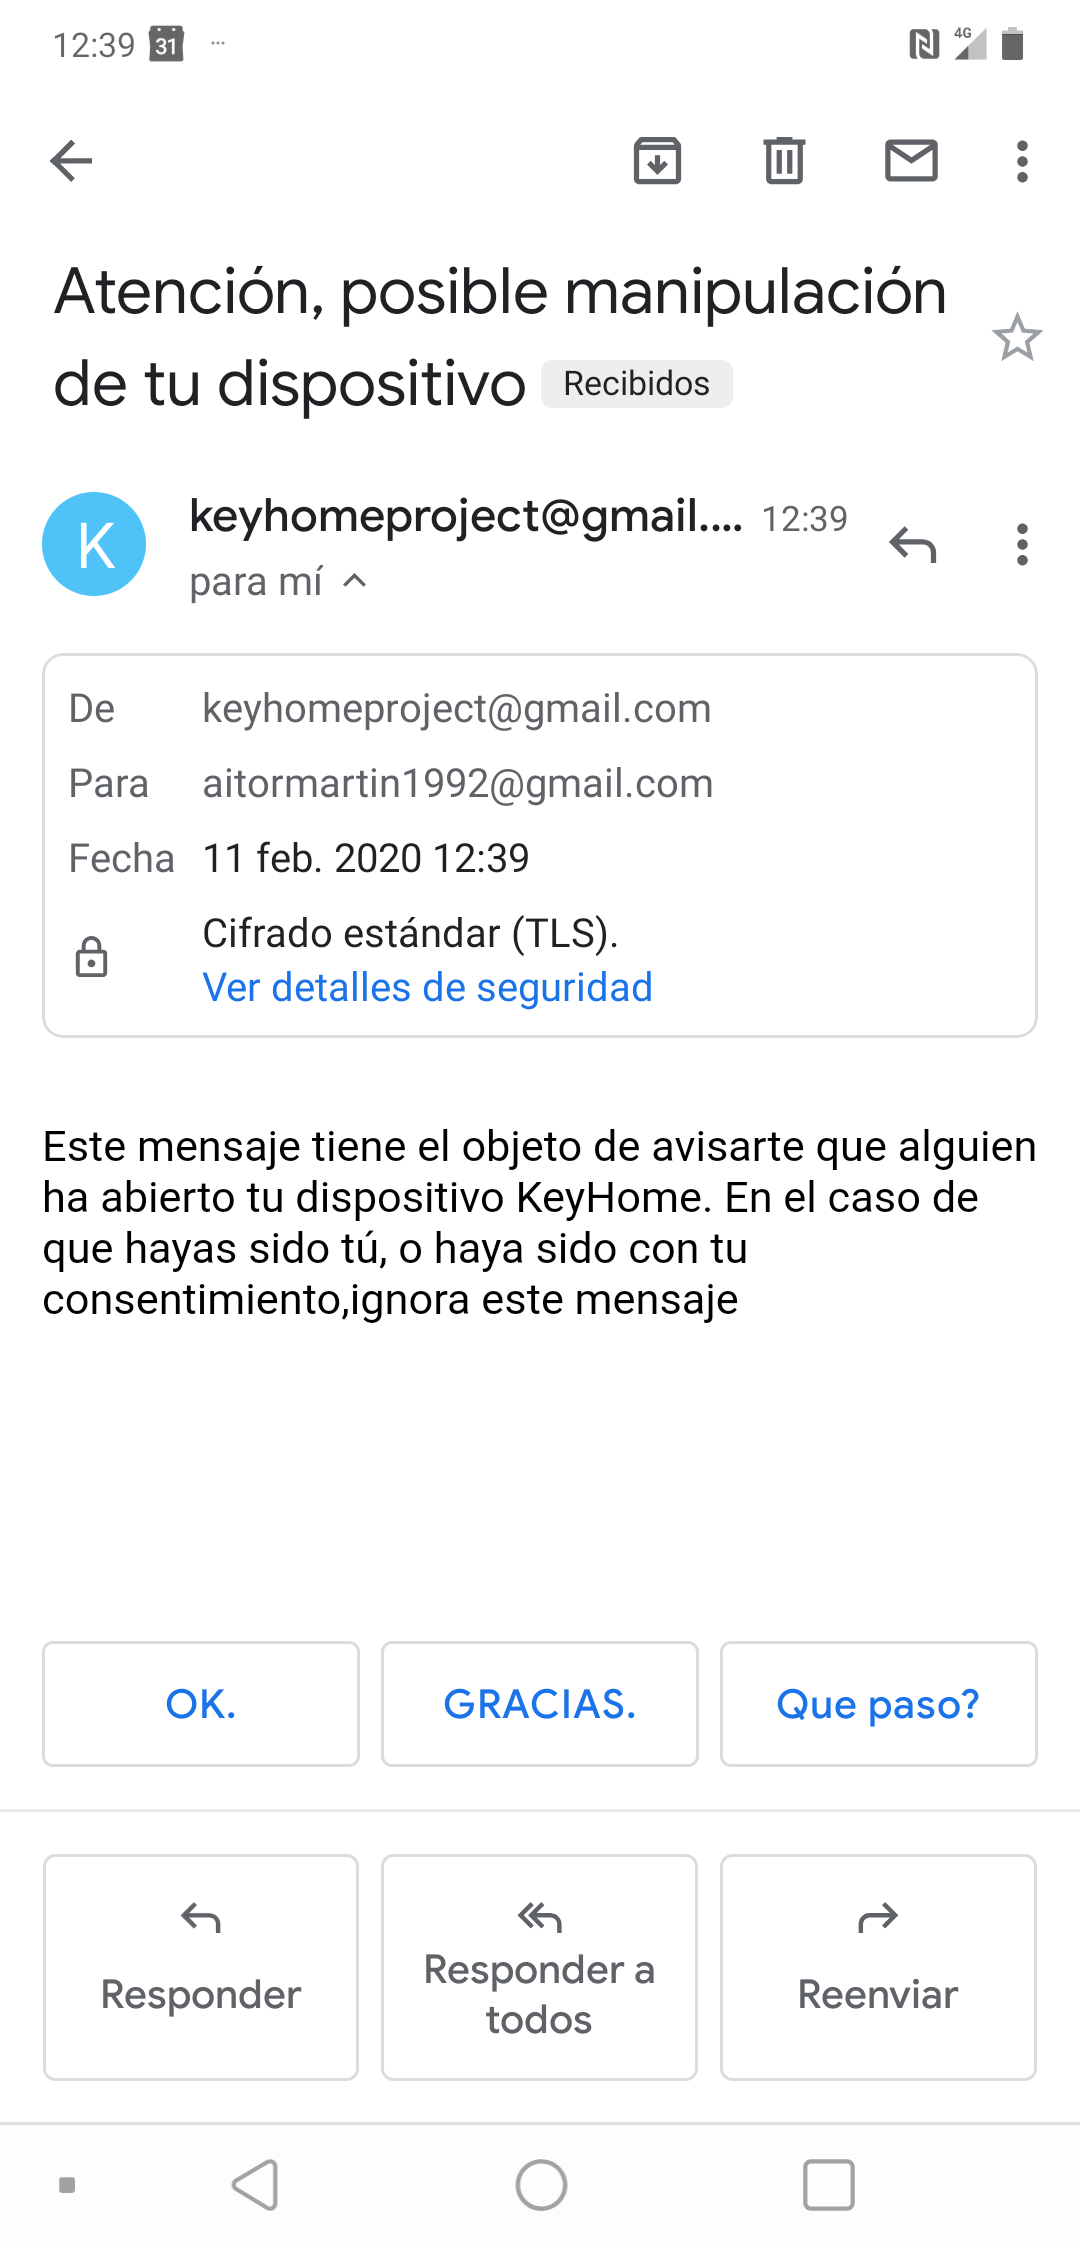
\includegraphics[scale=0.15]{fig/Aviso-ante-posible-manipulacion.png}
\caption{Aviso ante posible manipulación del dispositivo}
\label{fig:aviso-ante-posible-manipulacion}
\end{figure}

La desconexión, tanto a nivel eléctrico como de internet, del dispositivo, podría provocar múltiples situaciones negativas, como una posible manipulación o un cliente que no pudiera acceder a su vivienda. Para corregir esta situación, en la fase de desarrollo se decidió incluir un apartado en el que se avisara al propietario de forma remota. Para ello, se ha hecho uso de una plataforma llamada InitialState, que, tras la inclusión de ciertos scripts en la Raspberry Pi, recibe de forma continua señales de la ejecución del programa o programas que se deseen analizar. En la figura~\ref{fig:monitorizacion} puede observarse como, desde el ordenador, puede observarse de forma gráfica la frecuencia de trabajo de un programa en la Raspberry Pi.

\begin{figure}[tbp]
\centering
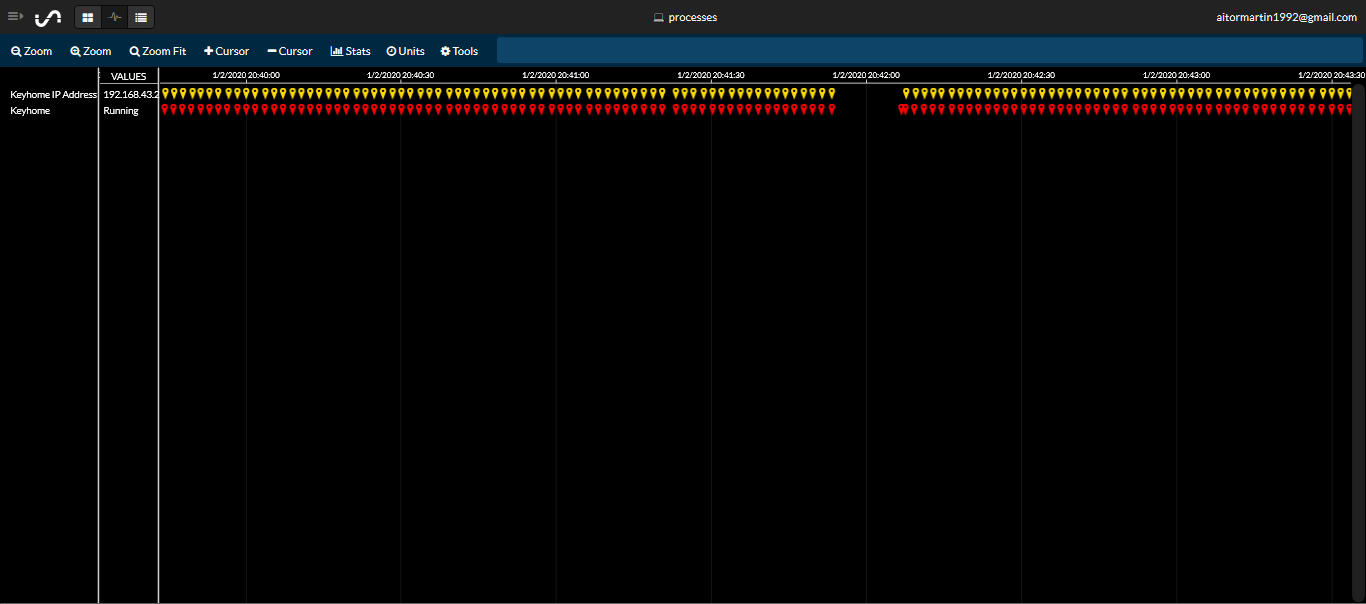
\includegraphics[scale=0.4]{fig/Monitorizacion.PNG}
\caption{Monitorización de la ejecución de un programa en la Raspberry Pi}
\label{fig:monitorizacion}
\end{figure}

En el caso de que se produzca una interrupción en el funcionamiento, el sistema de aviso alertará al propietario de la vivienda advirtiéndole de lo sucedido, tal como puede observarse en la figura~\ref{fig:aviso-ante-interrupcion-del-funcionamiento}. De esta manera, el anfitrión tendrá constancia de lo sucedido y podrá tomar las medidas que considere oportunas, como puede ser intercambiar la microSD de la Raspberry Pi para salvar posibles manipulaciones que pudieran haber ocurrido, o incluir por medio de su panel de control en Telegram las reservas que hubieran llegado en ese periodo de inactividad.

\begin{figure}[tbp]
\centering
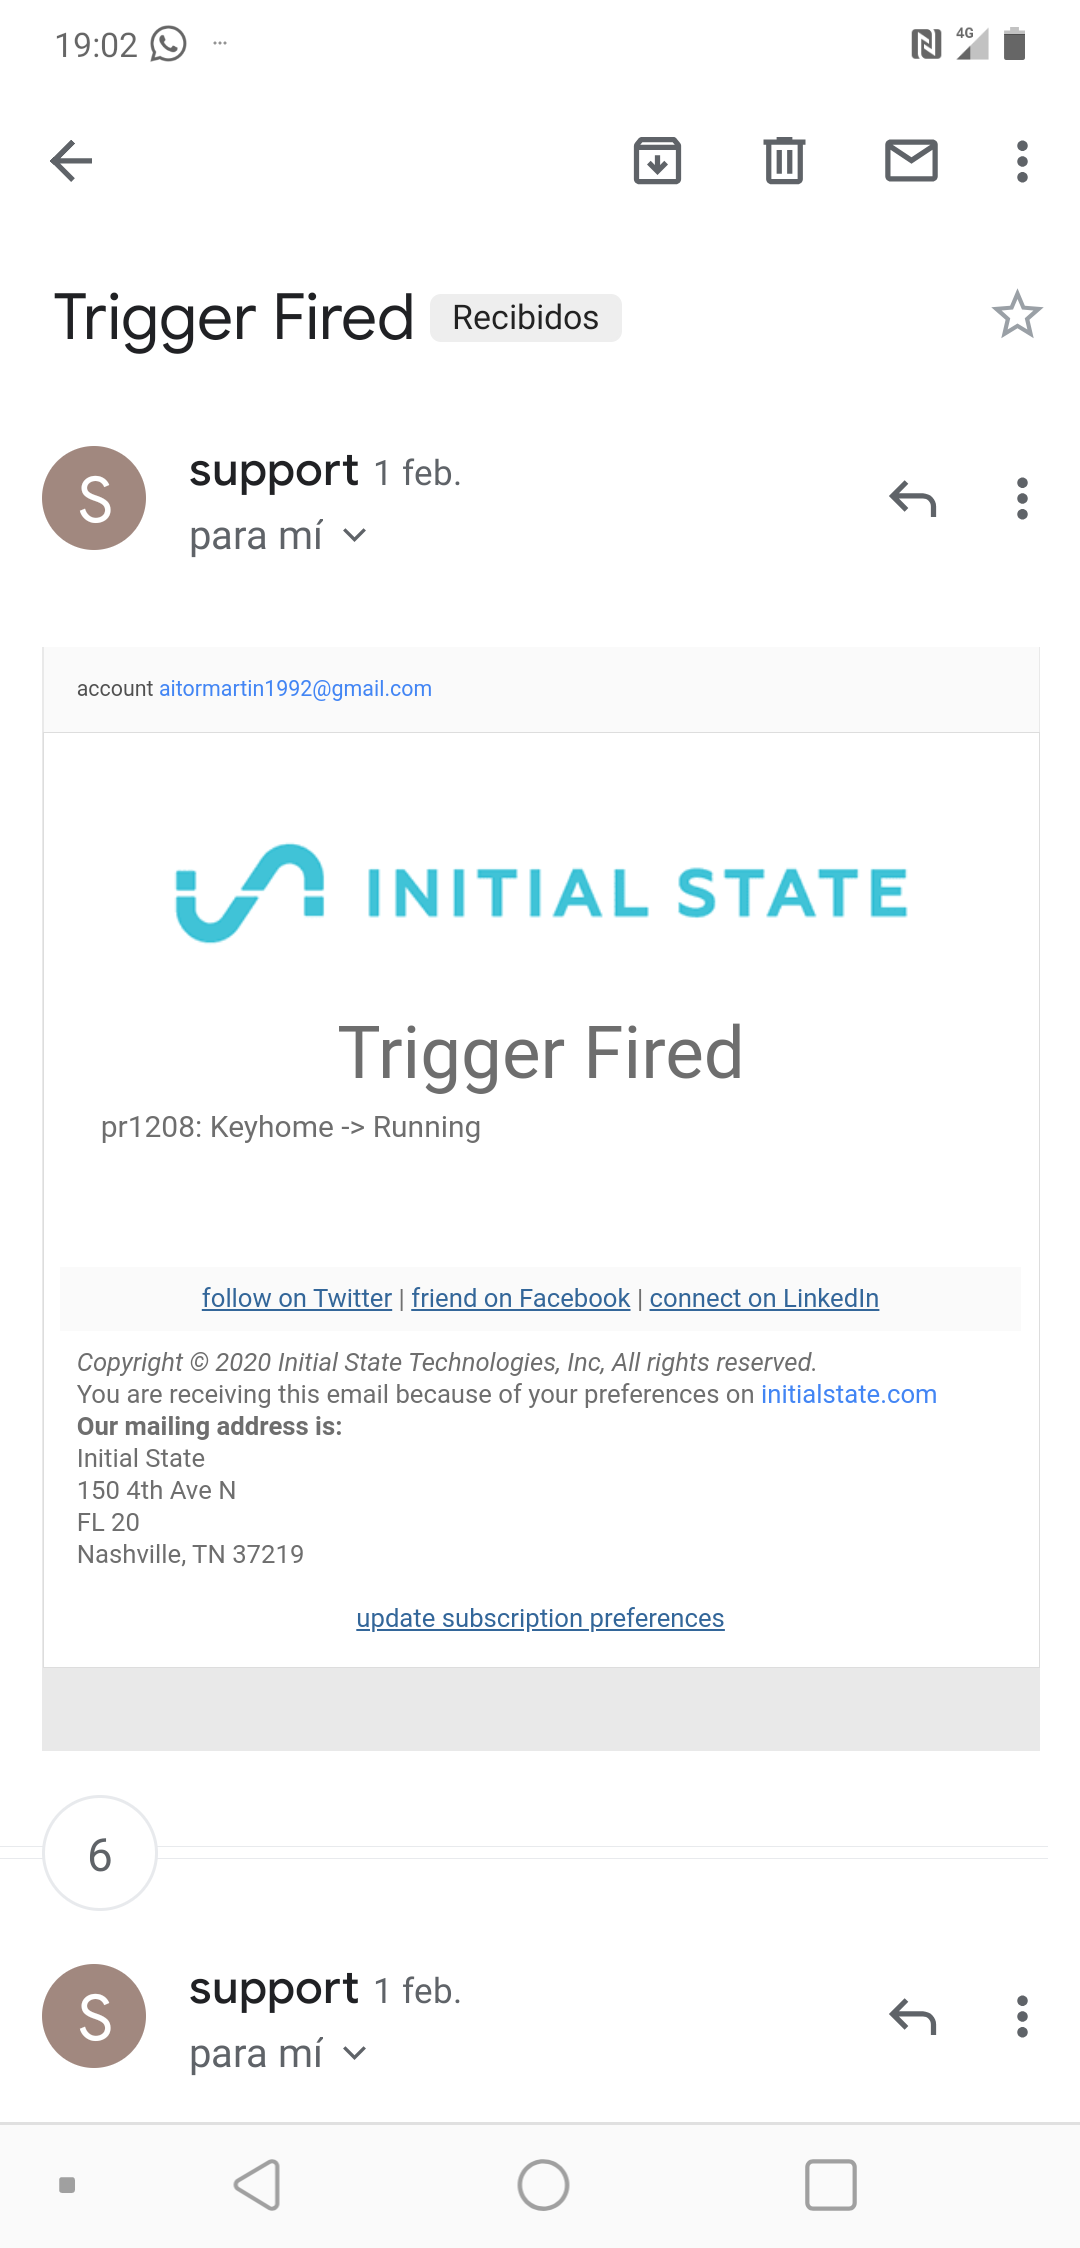
\includegraphics[scale=0.15]{fig/aviso-ante-interrupcion-del-funcionamiento.png}
\caption{Aviso ante una interrupción del funcionamiento}
\label{fig:aviso-ante-interrupcion-del-funcionamiento}
\end{figure}

\fi

\if00
\chapter{Discusión de resultados}
\label{ch:discusion-resultados}

Los resultados obtenidos a lo largo del desarrollo de este trabajo de fin de grado han sido en gran medida satisfactorios. El objetivo de automatizar por completo la reserva de un apartamento turístico ha sido llevado a cabo con éxito. Se presenta como resultado, por tanto, un producto funcional que ofrece un servicio adecuado y seguro para llevar a cabo la labor que es objeto de este proyecto.

No obstante, como todo avance tecnológico, la investigación y el desarrollo se han encontrado con aspectos positivos y también negativos, que vale la pena mencionar para poner en situación al lector y hacer que tenga una comprensión más profunda sobre el tema que se está tratando.

\section{Aspectos positivos}
\subsection{Instalación sencilla}
Uno de los aspectos positivos que vale la pena considerar es el hecho de que la instalación para el usuario final del dispositivo resultante de este proyecto tiene un carácter bastante sencillo. Únicamente deberá instalarse el aparato junto al portero automático conectado a un enchufe por medio de un cargador tipo USB micro B, disponible en multitud de comercios. El resto de la instalación consiste tan solo en conectar la hembra del conector mini jack en el telefonillo y poner cada uno de sus bornes en contacto con los puertos que permitan la apertura de la cerradura eléctrica desde el portero automático. Por ello, se obtiene un producto que puede instalarse en pocos minutos sin necesidad de conocimientos profundos en materia eléctrica o informática.
\subsection{Uso intuitivo}
El proyecto se ha desarrollado con éxito permitiendo tanto la gestión de la vivienda como el acceso a usuarios finales desde la aplicación de mensajería instantánea Telegram. El hecho de que sea la mensajería instantánea la que intermedie en todo momento hace que se presente un producto intuitivo y fácil de usar para multitud de usuarios que, en su vida diaria ya están acostumbrados a tratar con este tipo de aplicaciones.
\subsection{Producto seguro}
El resultado que se expone en este documento ha trabajado la seguridad en todos los aspectos posibles, desde su nivel más físico, impidiendo el acceso a la Raspberry Pi por medio de un diseño de impresión 3D protegido con candado, hasta sus niveles más sofisticados, avisando al administrador en caso de que se produzca una apertura o de que cualquier programa interrumpa su correcto funcionamiento. Este punto pone de manifiesto la importancia que se le da a la hora de proteger las residencias de aquellas personas que puedan interesarse por el producto.
\section{Aspectos negativos}
\subsection{Un mercado hermético}
Cabe destacar, sin embargo, que las posibilidades de aplicaciones que ampliarían la escalabilidad de este proyecto se ven comprometidas por la propia forma en que se estructura el mercado de las vivienda de uso turístico. En España, este negocio multimillonario es controlado y dirigido principalmente por 2 empresas (Booking y Airbnb) las cuales son bastante restrictivas a la hora de permitir trabajar con sus APIs.

Tan solo unas pocas empresas, que actúan como channel managers, tienen la posibilidad de trabajar con estos gigantes haciendo aplicaciones que actualicen los precios, gestionen las reservas, automaticen los registros de huéspedes para la policía, y otras muchas actividades que resultan de gran utilidad para los anfitriones. 

Este hecho provoca que la manera de trabajar para coger las reservas haya consistido, tal como se explica en el apartado de desarrollo del presente trabajo de fin de grado, en extraer la información necesaria de los correos electrónicos que notifican la información a los anfitriones. Este método, aunque se ha podido comprobar en este trabajo que funciona de manera correcta, no es la forma más eficiente de hacerlo, ya que podrían surgir problemas como el hecho de que las empresas de alquiler vacacional oculten información como las fechas de reserva o el número de reserva en los correos electrónicos, permitiendo tan solo acceder a los mismos desde el panel de administración de cada plataforma.

\subsection{Adaptación con cerraduras electromecánicas}
Una característica adicional que, por razones principalmente de coste, habría sido interesante llevar a cabo, sería la adaptación del sistema desarrollado con cerraduras inteligentes motorizadas. Activar la apertura con este tipo de cerraduras permitiría que no solo se emplearan cerraduras eléctricas en las viviendas donde se desee adaptar este sistema, si no que podría adaptarse a todo tipo de puertas y cerraduras, ofreciendo de esa manera, mayor seguridad ante robos o posibles allanamientos al usar infraestructuras más seguras.



\fi

\if00
\chapter{Conclusiones}
\label{ch:conclusiones}

Este trabajo de fin de grado ha concluido con éxito todos los objetivos propuestos en su apartado correspondiente. A nivel físico, se ha creado un circuito electrónico básico que, con la incorporación del software desarrollado, es capaz de cumplir con su cometido realizando la apertura de la cerradura eléctrica en los momentos que han sido planteados.

Adicionalmente, se han desempeñado exitosamente todas las tareas de desarrollo de software que se habían propuesto, tanto a nivel de funcionalidad, permitiendo la gestión integral de la vivienda y el acceso de los huéspedes, como a nivel de seguridad, teniendo en cuenta todos los posibles peligros que se consideraron en el análisis de este proyecto.

Como conclusión, se expone de este trabajo un proyecto completamente funcional que resuelve las tareas descritas y ofrece un servicio de utilidad a los posibles anfitriones que deseen hacer uso del mismo.

No obstante, este trabajo también cuenta con mejoras que no han sido tratadas, por cuestiones de tiempo y económicas, como son la implantación de este sistema en cerraduras inteligentes motorizadas o la integración de servicios de cálculo de precios, unificación de calendarios y otros servicios que pudieran hacer todavía más integral y útil este proyecto. Estas funcionalidades podrían ser tenidas en cuenta en una posible línea de investigación futura, que se apoye sobre el trabajo de este documento y la tecnología del momento.

Otros aspectos que serían relevantes para la evolución de este sistema a la hora de llevarlo a la realidad, sería la respuesta del propio público a la hora de utilizar estos sistemas automatizados. Todas las aplicaciones tecnológicas tienden a evolucionar con diferentes versiones, adaptándose a las necesidades del mercado según se van conociendo. En este caso no sería distinto, y la única forma de ver las mejoras que se deberían incluir, y los aspectos que se deberían considerar, sería probándolo directamente con clientes reales, que ayudarían a mejorar significativamente el valor de este producto.
\fi


% Los anexos pueden ir en la misma carpeta que el cuerpo del documento 
% porque eso facilita la migración de partes de un capítulo a un anexo.
\appendix\cleardoublepage
\if0
\hypertarget{ch:anexos}{%
    \chapter{Chuleta de \LaTeX{}}
\label{ch:latex}

\LaTeX{} es un formato textual para construir documentos complejos, cualquier tipo de documento complejo.  No es difícil, y de hecho está pensado para que personas sin formación en tipografía y composición puedan redactar documentos estéticamente impecables.  Pero necesita algo de tiempo para acostumbrarse a la filosofía.

Puedes acabar tu TFG simplemente imitando la redacción de este documento, pero seguro que puedes sacar más partido si aprendes algo de \LaTeX{}.  Hay muchas guías sencillas para empezar. Por ejemplo,~\cite{ernestoaranda2013} o~\cite{gastonsimone2002} son resúmenes suficientemente completos y sencillos.  En caso de que quieras ampliar tus conocimientos tendrás que empezar por el libro de Leslie Lamport~\cite{leslielamport1994}, el creador de \LaTeX{}.  Procura complementarlo con~\cite{latexcompanion2004} y, especialmente, navegar por el \href{https://ctan.org}{CTAN} (\emph{Comprehensive \TeX{} Archive Network}).  CTAN es un repositorio enorme de paquetes, que facilitan la edición de todo tipo de detalles.  Desde las cabeceras de página, hasta la creación de enlaces hipertexto o el manejo de colores.

En este anexo se incluye un pequeño recetario, extraído de la plantilla de Fernando Castillo, que puedes usar a modo de recordatorio rápido, pero procura utilizar una referencia más completa cuando empieces a editar el documento.

\warning{Este recetario no es un libro de \LaTeX{}, ni es para sentarse a leerlo, es para usarlo cuando lo necesites.  No te mostramos cómo se escribe en \LaTeX{} cada ejemplo, sino que directamente lo hacemos.  Cuando necesites hacer algo semejante, mira el código de este documento en \url{https://github.com/FranciscoMoya/eii-tfg}}

\section{Texto} 
\label{sec:texto}

\noindent En esta sección se muestran ejemplos de efectos de texto.

\begin{description}
\item[\texttt{textbf}] \textbf{Texto en negrita.}

\item[\texttt{textit}] \textit{Texto en cursiva.}

\item[\texttt{underline}] \underline{Texto subrayado.}

\item[\texttt{large}] {\large Texto grande}

\item[\texttt{Large}] {\Large Texto más grande}

\item[\texttt{LARGE}] {\LARGE Texto mucho más grande}

\item[\texttt{textsc}] \textsc{Texto en versalitas}

\item[\texttt{textsf}] \textsf{Texto en fuente sans-serif}

\item[\texttt{texttt}] \texttt{Texto en fuente mono-espaciada}
\end{description}

A veces resulta útil este tipo de texto para funciones de programación o código fuente. Por ejemplo:

\begin{verbatim}
    [x,y]=function(t,z) 
\end{verbatim}

\subsection{Listas numeradas y con viñetas} 

Listas numeradas. Se utilizan cuando la posición que ocupan los elementos es importante, para contar los elementos, o cuando se necesita añadir referencias a algunos de los elementos.

\begin{enumerate}
\item diodos
\item transistores
    \begin{enumerate}
    \item transistores pnp
    \item transistores npn
    \item operacionales
    \end{enumerate}
\item operacionales
\end{enumerate}

Listas con viñetas. Se utilizan cuando la posición concreta de los elementos no es importante:

\begin{itemize}
\item diodos
\item transistores
    \begin{itemize}
    \item transistores pnp
    \item transistores npn
    \item operacionales
    \end{itemize}
\item operacionales
\end{itemize}

\subsection{Acrónimos}

Si quieres lista de acrónimos debes marcar los acrónimos con una etiqueta especial.  Por ejemplo, así se pondría la primera vez un \ac{CD}.  Una vez que se ha usado el acrónimo, ya se puede usar en forma abreviada, como en~\acs{CD}.  Marca incluso en este caso los acrónimos, porque así el PDF permitirá navegar a la definición pinchando sobre él.

\section{Figuras}
\label{sec:figuras}

En esta sección se muestran algunos ejemplos de figuras.  La fig.~\ref{fig:figurita-ejemplo} es un ejemplo de \emph{Encapsulated PostScript}.  Se trata de un formato vectorial, que no se degrada al escalarlo.  Este tipo de formatos son los ideales para usar con \LaTeX{}.  Utiliza siempre que puedas imágenes en formato EPS o PDF.

\begin{figure}[hbtp]
\centering
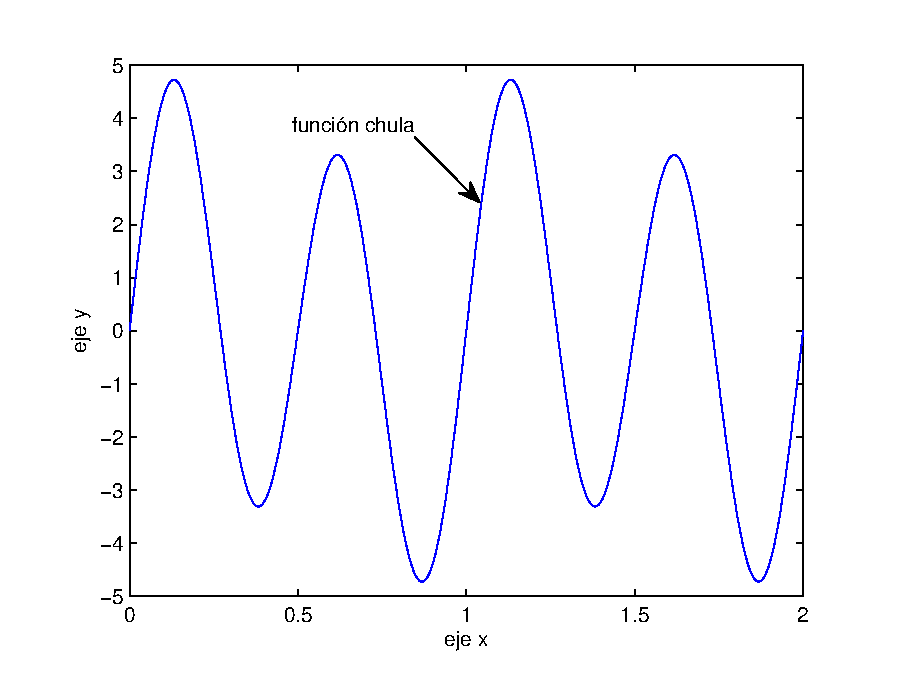
\includegraphics[scale=0.5]{ejemplo.eps}
\caption{Figurita ejemplo}
\label{fig:figurita-ejemplo}
\end{figure}

La forma de incluir la figura es simple:

\begin{lstlisting}[language={[LaTeX]TeX},frame=none,numbers=none]
\begin{figure}
\centering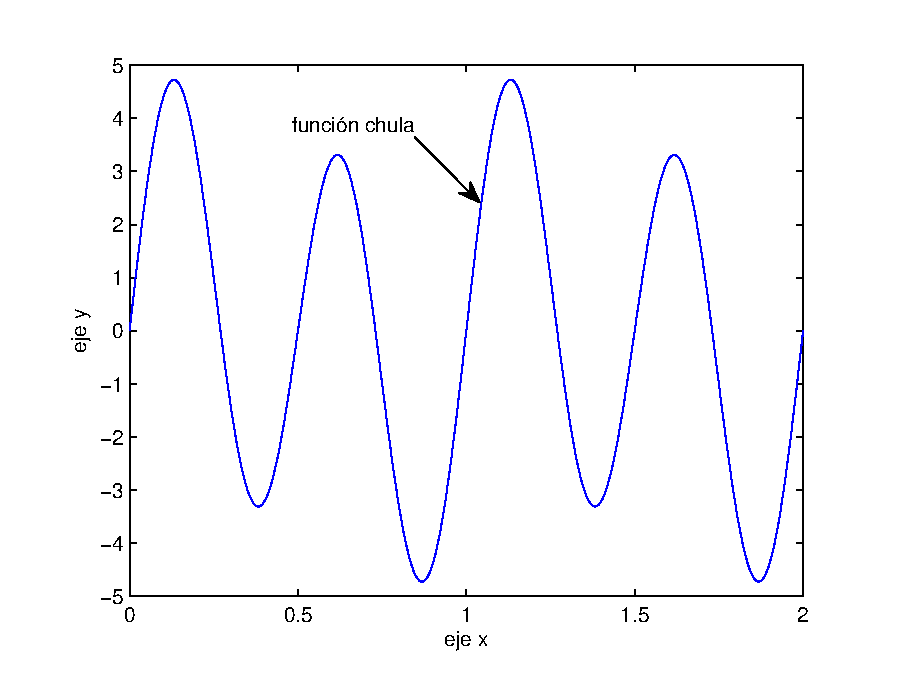
\includegraphics[width=6cm]{ejemplo.eps}
\caption{Figurita ejemplo}
\label{fig:figurita-ejemplo}
\end{figure}
\end{lstlisting}

El entorno \texttt{figure} crea un cuadro flotante, con todo el contenido de la figura, que \LaTeX{} coloca en el sitio menos malo.  La \texttt{caption} es el pie de la figura y la \texttt{label} es la etiqueta que nos permitirá referirnos a ella en el texto (con la orden \texttt{ref}).

\LaTeX{} utiliza un algoritmo nada evidente para colocar las figuras de manera que sea estéticamente agradable.  Pero tú puedes influir en las preferencias de colocación.  El entorno \texttt{figure} tiene un parámetro opcional entre corchetes que indica las opciones de colocación.  Por defecto es \texttt{[tbp]}, que equivale a \emph{top, bottom, page}.  Eso quiere decir que intenta primero ponerla a comienzo de página.  Si no lo consigue, al final de una página.  Y si así tampoco lo consigue, en una página entera, solo para la figura.  En este ejemplo utilizo las opciones \texttt{[hbtp]} para que intente la secuencia \emph{here, bottom, top, page}.  En este caso prefiero que la ponga debajo antes que arriba, para que no aparezca en una sección anterior.

Con \LaTeX{} puedes conseguir que las figuras no se muevan en absoluto, pero eso deja documentos extremadamente descompensados.  No lo hagas nunca.  Es mejor mover ligeramente la figura en el texto o incluso re-escribir parte del texto, antes de forzar la posición.  De todas formas, si no me quieres hacer caso, en la fig.~\ref{fig:figurita-ejemplo-2}  tienes un ejemplo que fuerza la posición.

\begin{figure}[H]
\centering
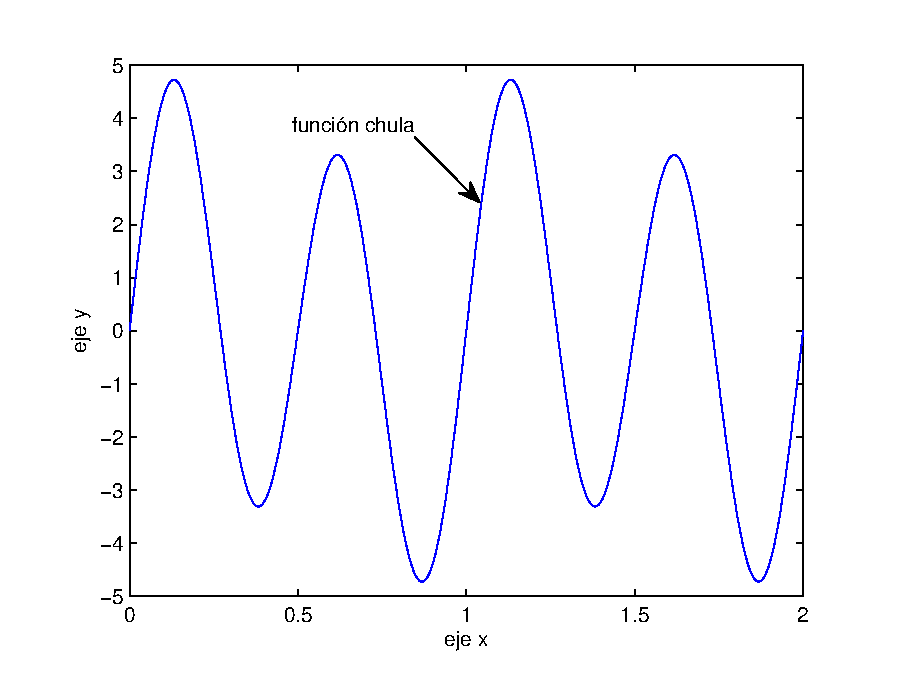
\includegraphics[scale=0.5, angle=15]{ejemplo.eps}
\caption{Figurita ejemplo 2}
\label{fig:figurita-ejemplo-2}
\end{figure}

Para poder poner figuras que no son de elaboración propia es necesario primero obtener permiso del autor y, además, añadir la fuente al pie de foto. Hay muchas guías de estilo que explican en detalle cómo hacerlo. Por ejemplo, la \emph{American Psychological Association} tiene un \href{https://www.lib.sfu.ca/help/research-assistance/format-type/online-images/citing#citing-images-in-apa}{capítulo específico de su manual de publicaciones}.  El manual de la APA se usa extensivamente en todo tipo de literatura científica.

\begin{figure}[htb]
\centering
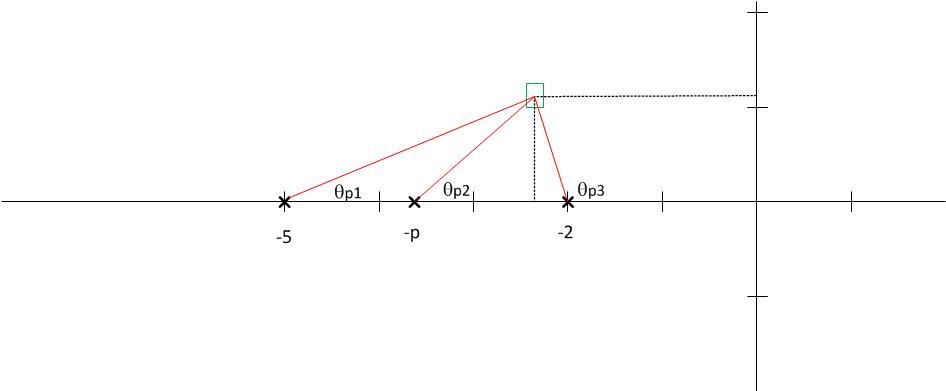
\includegraphics[scale = 0.5]{ejemplo2.jpg}
\caption{Figurita ejemplo 3. Extraída de la plantilla de TFG de Fernando Castillo. \copyright 2018 Fernando Castillo. Reproducida con permiso.}
\label{fig:figura-ejemplo-3}
\end{figure}

\warning{Fíjate bien.  No se citan las imágenes como si se tratara de referencias bibliográficas.  No debe haber pie de página (orden \texttt{footnote}) ni cita (orden \texttt{cite}) en un pie de foto (\texttt{caption}).  La atribución de la obra debe estar al mismo nivel que la obra usada.  Por eso debe atribuirse completamente en el pie de foto.  Si no te gusta como queda haz tus propias imágenes.}

Se puede controlar el escalado de la imagen y el ángulo de forma muy sencilla, con las opciones de la orden \texttt{includegraphics}.  En la fig.~\ref{fig:figura-ejemplo-3} se muestra un ejemplo de figura escalado a un 30\%.  La orden \texttt{includegraphics} ajusta los parámetros de la imagen para mantener la relación de aspecto original, si esto es posible.  Esto hace que podamos especificar simplemente el ancho o el alto deseado, que va a ser lo más habitual.  En mi opinión, las opciones más frecuentes de \texttt{includegraphics} son, por orden:

\begin{figure}
\centering
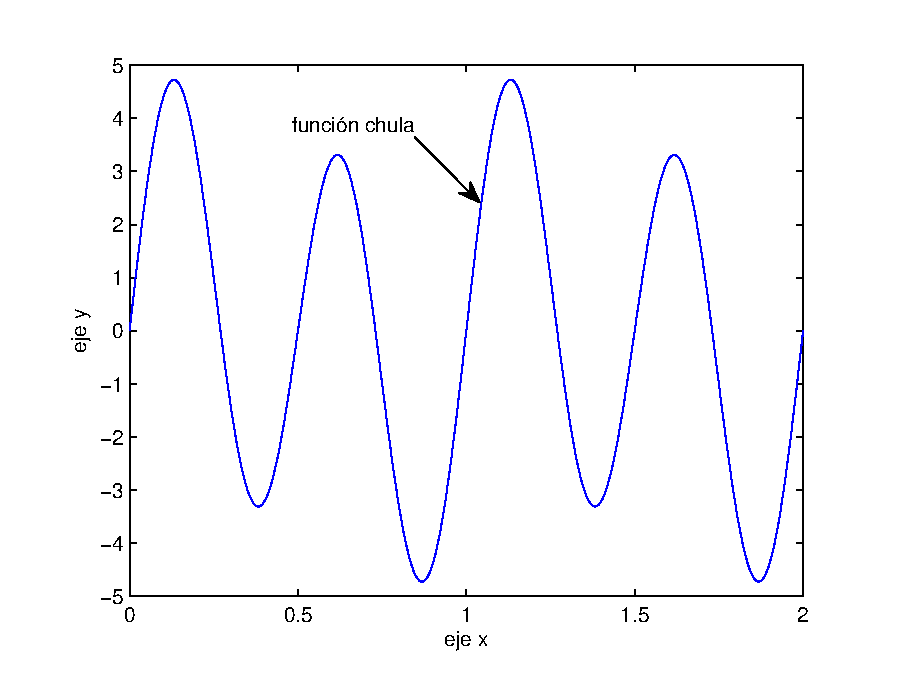
\includegraphics[width=\textwidth]{ejemplo.eps}
\caption{Figura ejemplo que ocupa todo el ancho del texto.}
\label{fig:figura-ejemplo-4}
\end{figure}

\begin{description}
\item[\texttt{width}]  Fija el ancho de la imagen.  Puede ser un tamaño absoluto en centímetros (\texttt{cm}), milímetros (\texttt{mm}) o puntos PostScript (\texttt{pt}).  Por ejemplo,  \verb|width=1.5cm|.  También puede ser un tamaño relativo a cualquier medida del documento.  Por ejemplo, \verb|width=0.5\textwidth| sería una figura que ocupe la mitad del ancho del texto.

\item[\texttt{height}] Fija la altura de la imagen.  Es similar a \texttt{width} pero con la altura.  Se puede especificar tanto altura como anchura, de manera que se modifica la relación de aspecto original.

\item[\texttt{scale}] Utiliza un factor de escala para la imagen.  Puede ser mayor de 1 para ampliar la imagen.

\item[\texttt{angle}] Gira la imagen un número de grados determinado.  Si el número es negativo el giro es en sentido horario.  Si es positivo el giro es antihorario.
\end{description}


En la fig.~\ref{fig:figura-angulo-30} se muestra un ejemplo de figura girada 30.

\begin{figure}[btp]
\centering
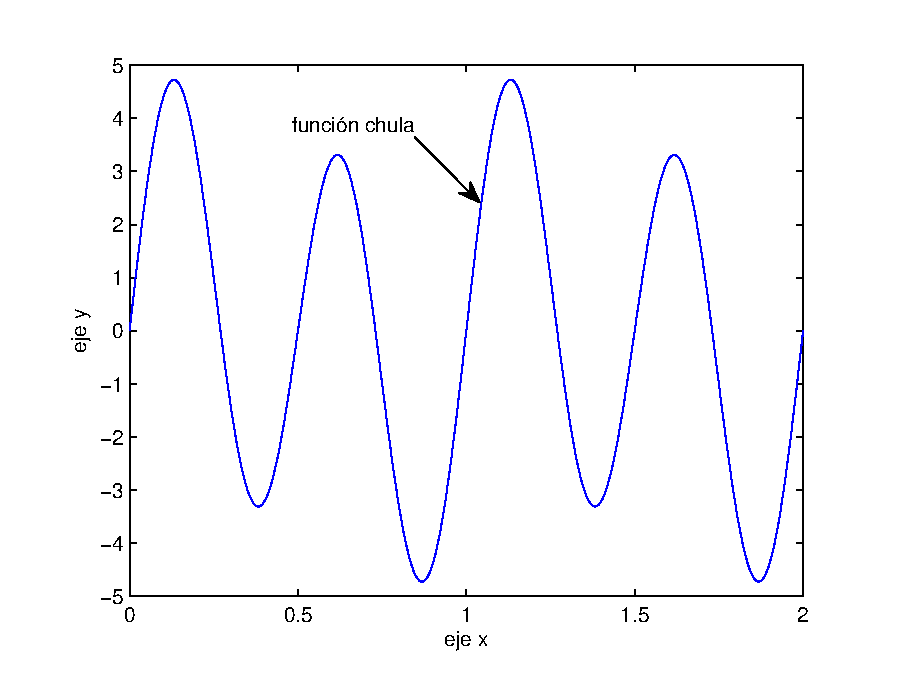
\includegraphics[width=.3\textwidth,angle=-30]{ejemplo.eps}
\caption{Figura ejemplo de rotación.}
\label{fig:figura-angulo-30}
\end{figure}

Una característica interesante del entorno \texttt{figure} es que permite definir sub-figuras con la orden \texttt{subfigure} o el entorno del mismo nombre.  La colocación de las sub-figuras es prácticamente automática.  Un ejemplo puede verse en la figura~\ref{fig:matriz-figuras}.

\begin{figure}[htbp]
\centering
\subfigure[figurita1]{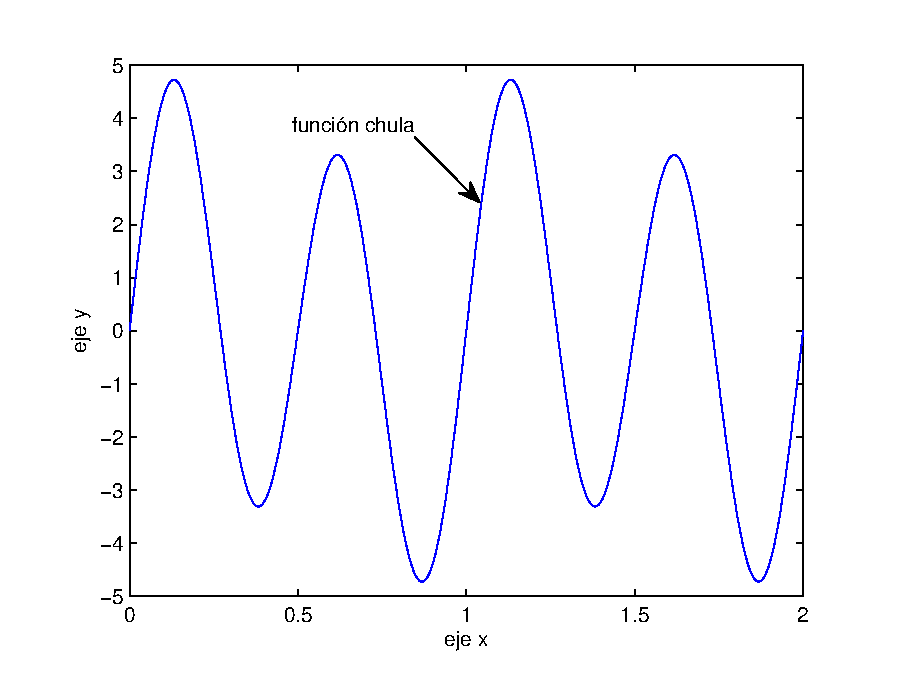
\includegraphics[width=40mm]{ejemplo.eps}}
\subfigure[figurita2]{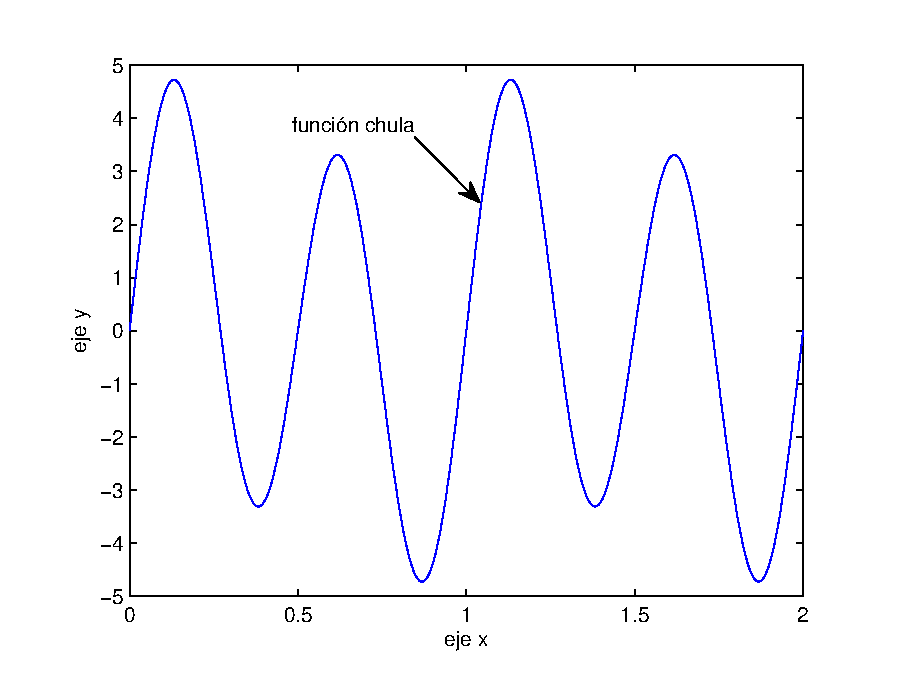
\includegraphics[width=40mm]{ejemplo.eps}}
\subfigure[figurita3]{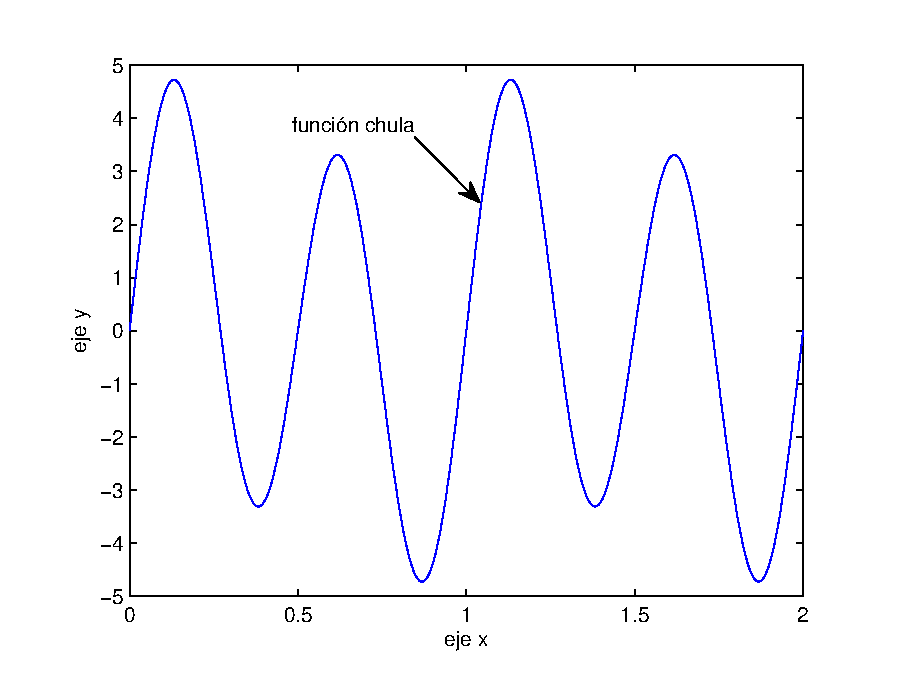
\includegraphics[width=80mm]{ejemplo.eps}}
\caption{Matriz de figuras} 
\label{fig:matriz-figuras}
\end{figure}

Una subfigura puede referenciarse a partir de la referencia a la figura.  Por ejemplo, la figura~\ref{fig:matriz-figuras}(a) es igual que la figura~\ref{fig:matriz-figuras}(b). Sin embargo, cuando las figuras son muy complejas, es posible que se prefieran esquemas más automáticos.  En \href{https://tex.stackexchange.com/questions/181225/how-to-reference-to-subfigure-in-latex}{StackExchange} encontrarás soluciones a éste y otros problemas con mucha facilidad.

En general, he tratado de mantener un compromiso entre el número de características incluidas y la facilidad de uso de la plantilla.  Las figuras muy complejas es algo que prefiero evitar, así que en el estilo de la plantilla no incorpora el paquete \texttt{subcaption}.

\section{Tablas} 
\label{sec:tablas}

En esta sección se muestran algunos ejemplos de tablas.

\begin{table}[htb]
\centering
\vspace{2mm}
\begin{tabular}{|c|c|c|}
\hline
 Regulador & Función de Transferencia & orden  \\
 \hline
 P         & $\alpha_1$               & 2      \\
 \hline
\end{tabular}
\caption{Resultados de la simulación}
\label{tab:resultados-simulacion}
\end{table}

Las tablas en \LaTeX{} no son complejas pero puedes simplificar aún más usando un editor interactivo de tablas.  Por ejemplo, en \url{https://truben.no/table/} hay una aplicación \emph{online} para editar multitud de formatos de tablas.  Es especialmente útil para tablas complicadas.

En \LaTeX{} es bastante frecuente separar la cabecera del cuerpo de la tabla poniendo dos \texttt{hline}, como en la tabla~\ref{tab:sencilla}.

\begin{table}[htb]
\begin{center}
\begin{tabular}{|l|l|}
\hline
País     &    Ciudad \\ \hline \hline
España   &    Madrid \\ \hline
España   &    Valencia \\ \hline
Francia  &    París \\ \hline
\end{tabular}
\caption{Tabla muy sencilla.}
\label{tab:sencilla}
\end{center}
\end{table}

La complejidad empieza cuando hay que expandir celdas para ocupar varias columnas o varias filas.  Por ejemplo, la tabla (\ref{tab:dificililla}) tiene una celda multi-columna y otra celda multi-fila.  En estos casos un editor interactivo como el de \href{https://truben.no/table/}{Peder Lång Skeidsvoll} puede ser de gran ayuda para un principiante.  Explora las opciones, no son evidentes al principio.

\begin{table}[htb] 
\centering
\begin{tabular}{|c|c|}
\hline
\multicolumn{2}{|c|}{Europa} \\
\hline
País  & Ciudad \\ \hline \hline
\multirow{2}{1.1cm}{España} & Madrid \\ \cline{2-2}
& Valencia \\ \hline
Francia & París \\ \hline
\end{tabular}
\caption{Fusionando celdas.}
\label{tab:dificililla}
\end{table}

Las tablas, al igual que las figuras, tienen un parámetro opcional entre corchetes que indican las preferencias de posición.  Se puede forzar pero, al igual que con las figuras, conduce a documentos muy descompensados.  Procura evitarlo.  Dentro de la tabla se define un entorno \texttt{tabular} que indica con su argumento obligatorio las columnas.  Este entorno es muy útil en cualquier organización matricial.  Se puede usar también para presentar las subfiguras de una figura, o para definir una matriz.

Las tablas muy largas deben dividirse en varias páginas.  En el estilo de este TFG hemos incluído el paquete \texttt{longtable}, que facilita enormemente escribir este tipo de tablas largas.  En ese caso, en lugar del entorno \texttt{table} y el entorno \texttt{tabular} se usaría solamente el entorno \texttt{longtable}, que es una especie de híbrido de los dos, con un montón de características opcionales.  Para ilustrar su uso reproducimos \href{https://texblog.org/2011/05/15/multi-page-tables-using-longtable/}{un ejemplo de TeXblog} en la tabla~\ref{tab:tabla-larga}.

\begin{center}
\begin{longtable}{|c|c|c|c|}
\caption{Un ejemplo de tabla larga}
\label{tab:tabla-larga}\\
\hline
\textbf{Primera} & \textbf{Segunda} & \textbf{Tercera} & \textbf{Cuarta} \\
\hline
\endfirsthead
\multicolumn{4}{c}%
{\scriptsize\textbf{\tablename\ \thetable}\ -- \textit{Continúa de la página anterior}} \\
\hline
\textbf{Primera} & \textbf{Segunda} & \textbf{Tercera} & \textbf{Cuarta} \\
\hline
\endhead
\hline \multicolumn{4}{r}{\textit{\scriptsize Continúa en la página siguiente}} \\
\endfoot
\hline
\endlastfoot
1 & 2 & 3 & 4 \\ 1 & 2 & 3 & 4 \\ 1 & 2 & 3 & 4 \\ 1 & 2 & 3 & 4 \\
1 & 2 & 3 & 4 \\ 1 & 2 & 3 & 4 \\ 1 & 2 & 3 & 4 \\ 1 & 2 & 3 & 4 \\
1 & 2 & 3 & 4 \\ 1 & 2 & 3 & 4 \\ 1 & 2 & 3 & 4 \\ 1 & 2 & 3 & 4 \\
1 & 2 & 3 & 4 \\ 1 & 2 & 3 & 4 \\ 1 & 2 & 3 & 4 \\ 1 & 2 & 3 & 4 \\
1 & 2 & 3 & 4 \\ 1 & 2 & 3 & 4 \\ 1 & 2 & 3 & 4 \\ 1 & 2 & 3 & 4 \\
1 & 2 & 3 & 4 \\ 1 & 2 & 3 & 4 \\ 1 & 2 & 3 & 4 \\ 1 & 2 & 3 & 4 \\
1 & 2 & 3 & 4 \\ 1 & 2 & 3 & 4 \\ 1 & 2 & 3 & 4 \\ 1 & 2 & 3 & 4 \\
1 & 2 & 3 & 4 \\ 1 & 2 & 3 & 4 \\ 1 & 2 & 3 & 4 \\ 1 & 2 & 3 & 4 \\
\end{longtable}
\end{center}
\section{Ecuaciones} 
\label{sec:ecuaciones}

Si hay algo donde \LaTeX{} es especialmente útil, es en las fórmulas matemáticas.  Prácticamente no hay otra opción cuando las fórmulas son relativamente complejas.  En esta sección se muestran algunos ejemplos de ecuaciones.

\begin{equation}
    \mathbf{v} = \left[
    \begin{array}{c}
        2 \\
        3 \\
        -4 
    \end{array}
    \right]
\end{equation}

En \LaTeX{} es trivial el uso de cualquier notación de vectores.  Tan solo hay que familiarizarse con las órdenes correspondientes.  Por ejemplo, en esta ecuación:

\begin{equation} 
\vec{F} = m \vec{a}
\label{eq:dinamica}
\end{equation}

\noindent donde $\vec{F}$ es la fuerza, $\vec{a}$ es la actitud y $m$ la masa.

Las ecuaciones pueden referenciarse igual que las figuras, las tablas o las secciones.  Por ejemplo, la ecuación~\ref{eq:dinamica2} \ldots

\begin{equation} 
\alpha_{\mathit{inicial}} = \beta^{\mathit{final}} + \gamma
\label{eq:dinamica2}
\end{equation}

Repara bien en cómo se escribe la ecuación anterior.  Una palabra (o más de una) en una fórmula debe ponerse con ayuda de las órdenes auxiliares \texttt{mathrm}, \texttt{mathit}, etc.  En caso contrario parecerá un conjunto de letras que representan símbolos que se multiplican entre sí.  Para más detalles consulta~\cite{andrewroberts2004}.

\begin{equation}
G(s)=\frac{(s^2+s+1)^2}{s^3+1}
\label{eq:dinamica3}
\end{equation}

El uso de letras griegas o símbolos matemáticos es también muy sencillo.  Tan solo hay que familiarizarse con la orden que los inserta.  Puede parecer difícil, pero basta con ojear una chuleta como \href{https://www.colorado.edu/physics/phys4610/phys4610_sp15/PHYS4610_sp15/Home_files/LaTeXSymbols.pdf}{ésta}\footnote{\url{https://www.colorado.edu/physics/phys4610/phys4610_sp15/PHYS4610_sp15/Home_files/LaTeXSymbols.pdf}}.

La ecuación~\ref{eq:transformacion} muestra un ejemplo de integral.  También es muy sencillo, puesto que la notación de los límites coincide con la de los subíndices y superíndices.

\begin{equation}
F(y) =  \int_{x_a}^{x_b} K(x,y) f(x) dx
\label{eq:transformacion}
\end{equation}

Cuando se necesita un entorno tabular dentro de un entorno matemático se utiliza el entorno \texttt{array}. La ecuación~\ref{eq:matriz} muestra un ejemplo.

\begin{equation}
\left(
\begin{array}{cccc}
1 & 0 & \cdots & 0 \\
0 & 1 & \cdots & 0 \\
\vdots & \vdots & \ddots & \vdots \\
0 & 0 & \cdots & 1
\end{array}
\right)
\label{eq:matriz}
\end{equation}

\section{Bibliografía, citas y referencias} 
\label{sec:bibliografia-citas}

Otro de los aspectos especialmente cuidados de \LaTeX{} es el manejo de bibliografía y citas.  En esta plantilla utilizamos el paquete \emph{biblatex}.  Es un paquete muy flexible que permite adaptarse a casi cualquier estilo de citas existente.  En los documentos de ingeniería no hay consenso en el estilo a utilizar.  Nosotros hemos configurado en la plantilla el estilo del IEEE, pero dependiendo del área específica de trabajo puede ser necesario cambiarlo. Consulta con tu tutor.

La bibliografía en \LaTeX{} se hace con ayuda de unos archivos auxiliares escritos en formato BibTeX.  Es otro formato textual, con una serie de campos que hay que rellenar.  Para la composición de entradas BibTeX lo más sencillo es utilizar un editor online, como la página \url{http://truben.no/latex/bibtex/}.  En principio todas las entradas de bibliografía que utilices en tu TFG deben ponerse en \texttt{bib/main.bib}.

En \LaTeX{} la forma más básica de cita consiste en emplear la orden \texttt{cite} con el campo clave que contiene todo registro de BibTeX.  Por ejemplo, según el trabajo~\cite{armas2011estimation} \ldots mientras que según~\cite{castillo2010design} el control es una cosa muy buena.  Pero hay muchas otras opciones de cita.  Consulta la \href{http://tug.ctan.org/info/biblatex-cheatsheet/biblatex-cheatsheet.pdf}{chuleta de Bib\LaTeX} para ver todas las posibilidades.  Entre las alternativas más frecuentes está la orden \texttt{parencite} con el campo clave que contiene el registro BibTeX y entre corchetes la página concreta.  Por ejemplo, según~\parencite[3]{armas2011estimation} bla bla.  Como ves, el aspecto visual es similar, pero añade la página a la que hacemos referencia.  Otra posibilidad es usar la orden \texttt{textcite} que añade los autores.  Por ejemplo, según~\textcite{armas2011estimation} bla bla.

Se puede personalizar el aspecto de las citas cambiando los parámetros \texttt{style} y \texttt{citestyle} del paquete \texttt{biblatex} en \texttt{sty/eiitfg.cls}.  En ingeniería el estilo más utilizado, con mucha diferencia, es el de IEEE, del que existen dos variantes, \texttt{ieee} y \texttt{ieee-alphabetic}.  La única diferencia entre ambos es que en el primero se usan números para identificar las referencias y en el segundo se utilizan iniciales de los apellidos de los autores.

Otros valores muy utilizados son \texttt{alphabetic}, \texttt{authoryear}, \texttt{apa}, \texttt{chem-acs}, \texttt{mla}, \texttt{phys}, \texttt{nature}, \texttt{science}.  Sin embargo te recomendamos que utilices una de las dos variantes del estilo IEEE porque incluye soporte de entradas BibTeX para patentes.

También se puede acceder a campos concretos del registro BibTeX, tales como el autor, el año o el título.  Por ejemplo, \citeauthor{armas2011estimation} escribió en \citeyear{armas2011estimation} el artículo \citetitle{armas2011estimation}.

Otro estilo más antiguo es el estilo de Vancouver, en el que se usan notas al pie.  En \LaTeX{} puede hacerse con la orden \texttt{footcite}.  Por ejemplo, según el profesor Armas~\footcite[3]{armas2011estimation} bla bla.  Todavía se ve este estilo en libros de historia, pero tiende al desuso porque rompe la linealidad del texto. En general, lo más importante es ser consistente, usa un estilo y solo un estilo en todo el documento.

\subsection{Lo que toda referencia tiene que tener}

Una referencia bibliográfica se utiliza como argumento de autoridad, para dar peso a tu propia argumentación.  Por tanto, hay tres elementos clave que siempre deben estar: 
\begin{itemize}
    \item El autor, puesto que palabras anónimas no dan peso a nada.  Recuerda que el autor es lo que da peso a tu argumento.  No cites artículos divulgativos, ni autores sin un mínimo prestigio en el campo de lo que afirman.
    \item El título, puesto que el lector debe poder buscar por sí mismo el documento original.
    \item La fecha, puesto que un mismo autor puede cambiar de opinión a lo largo de su vida.  Por ejemplo  John Maynard Keynes es Premio Nobel pero tiene numerosos escritos contradictorios.  Su opinión era bastante cambiante con el tiempo.
\end{itemize}

Si falta alguno de estos elementos no es una referencia y no se cita.  Se puede poner como una nota a pie de página (\texttt{footnote}) o como una URL en el cuerpo del texto, pero no como una referencia.

Por cierto, es conveniente citar las fuentes.  Es decir, debes tomarte la molestia de buscar quién dijo o inventó lo que citas y dónde lo publicó por primera vez.  Es la mínima cortesía que se debe tener con los colegas de profesión.  Supongo que tú también querrás crédito por tu trabajo en tu futuro profesional.
		
\section{Hojas de datos}
\label{sec:hojas-datos}

Las hojas de datos normalmente son archivos PDF.  En \LaTeX{} hay dos formas de insertar archivos PDF.  La más sencilla es utilizar la orden \texttt{includegraphics} que ya hemos visto en las figuras, pero solo se puede incrustar una página en cada llamada a \texttt{includegraphics}. 

Si el documento tiene varias páginas habría que insertar cada una de las páginas de interés con órdenes \texttt{includegraphics} independientes.  En el parámetro \texttt{page} podemos elegir la página a insertar.  Este método nos da el máximo control para poder poner pies de figura y el posicionamiento.  Sin embargo, cuando el documento tiene muchas páginas es un poco engorroso.  Para esos casos se puede utilizar la orden \texttt{includepdf} del paquete \emph{pdfpages}.

Para ilustrarlo veamos el mismo ejemplo, primero con \texttt{includepdf} y luego con \texttt{includegraphics}.

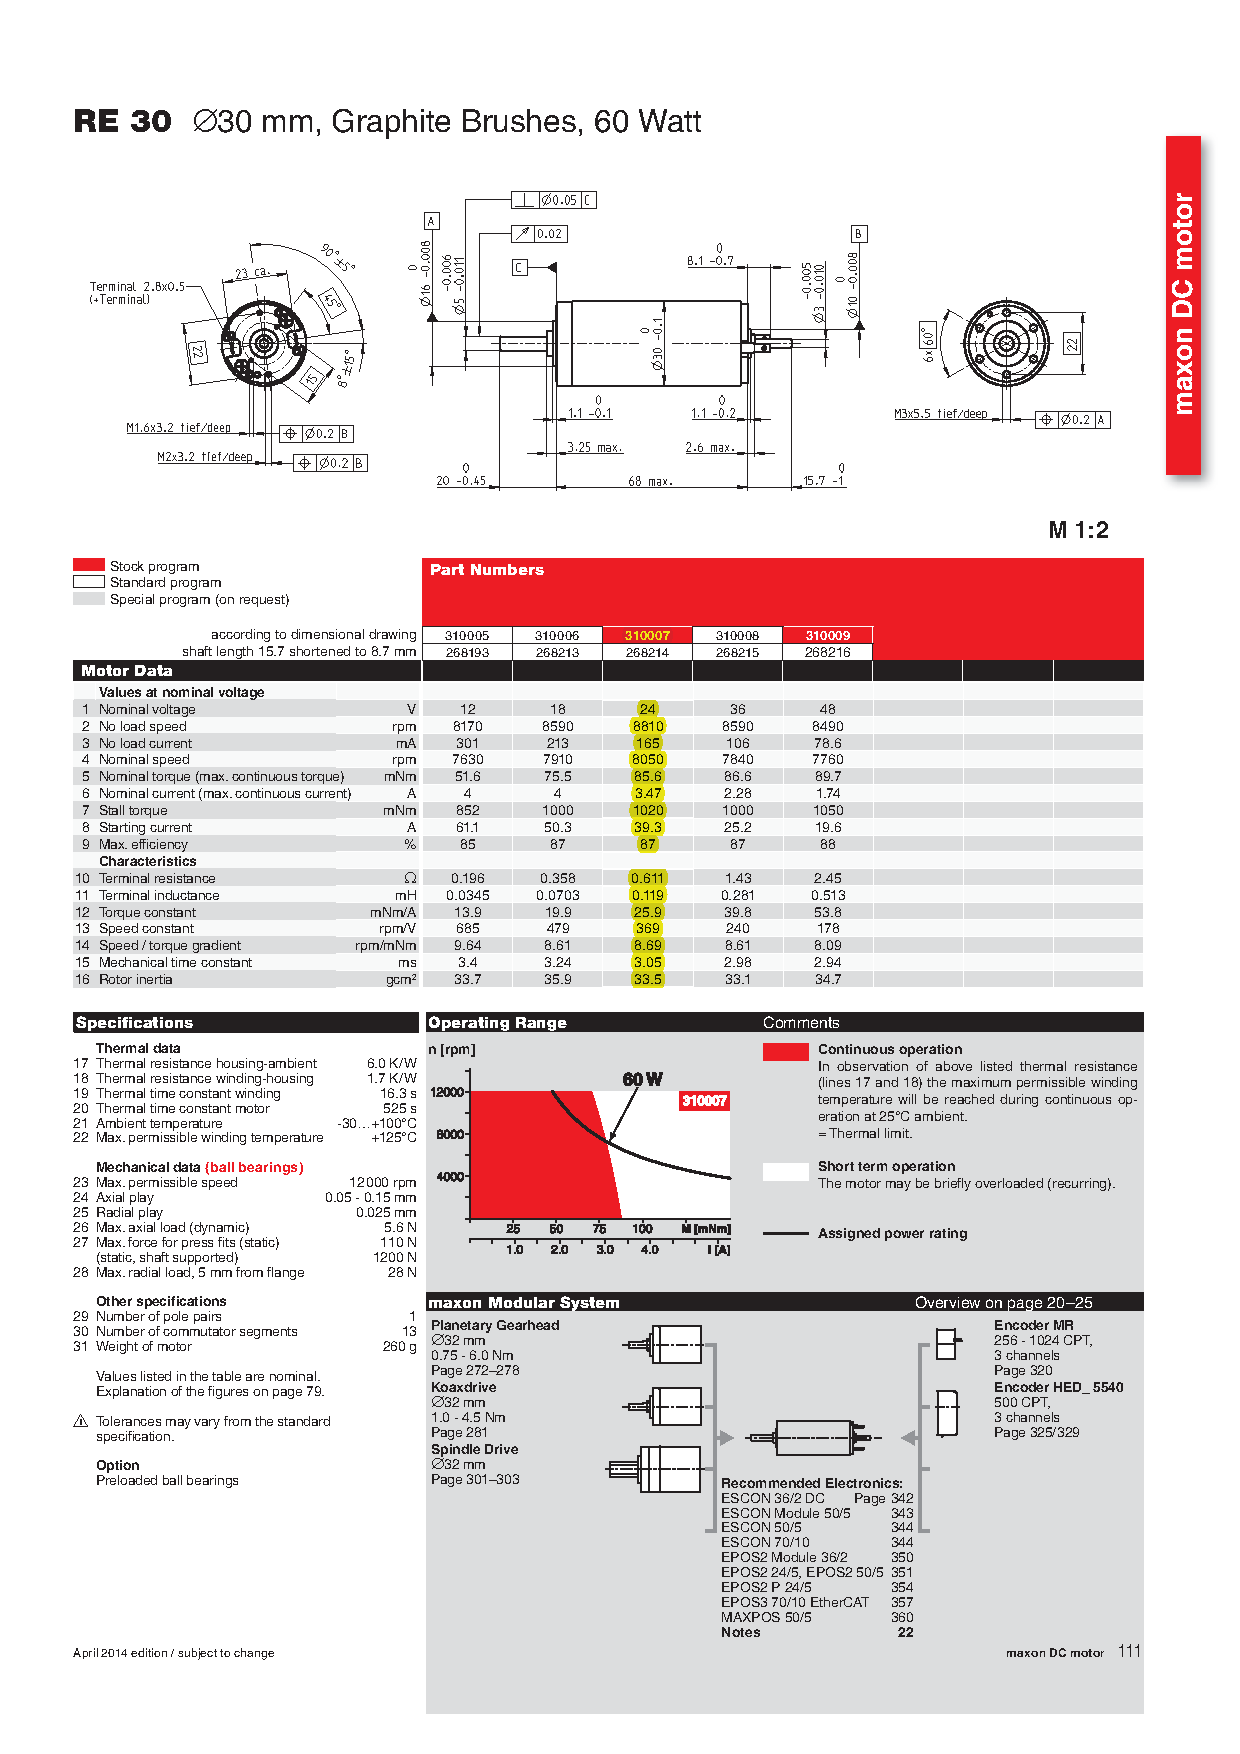
\includepdf[pages={1-},scale=0.8,pagecommand={}]{RE30.pdf}

La opción con \texttt{includegraphics} permite referirse a una página concreta y poner pies de figura.  Por ejemplo, en la figura~\ref{fig:hoja-datos} se muestra la hoja de especificaciones del motor empleado.

\begin{figure}[!ht]
\centering
\fbox{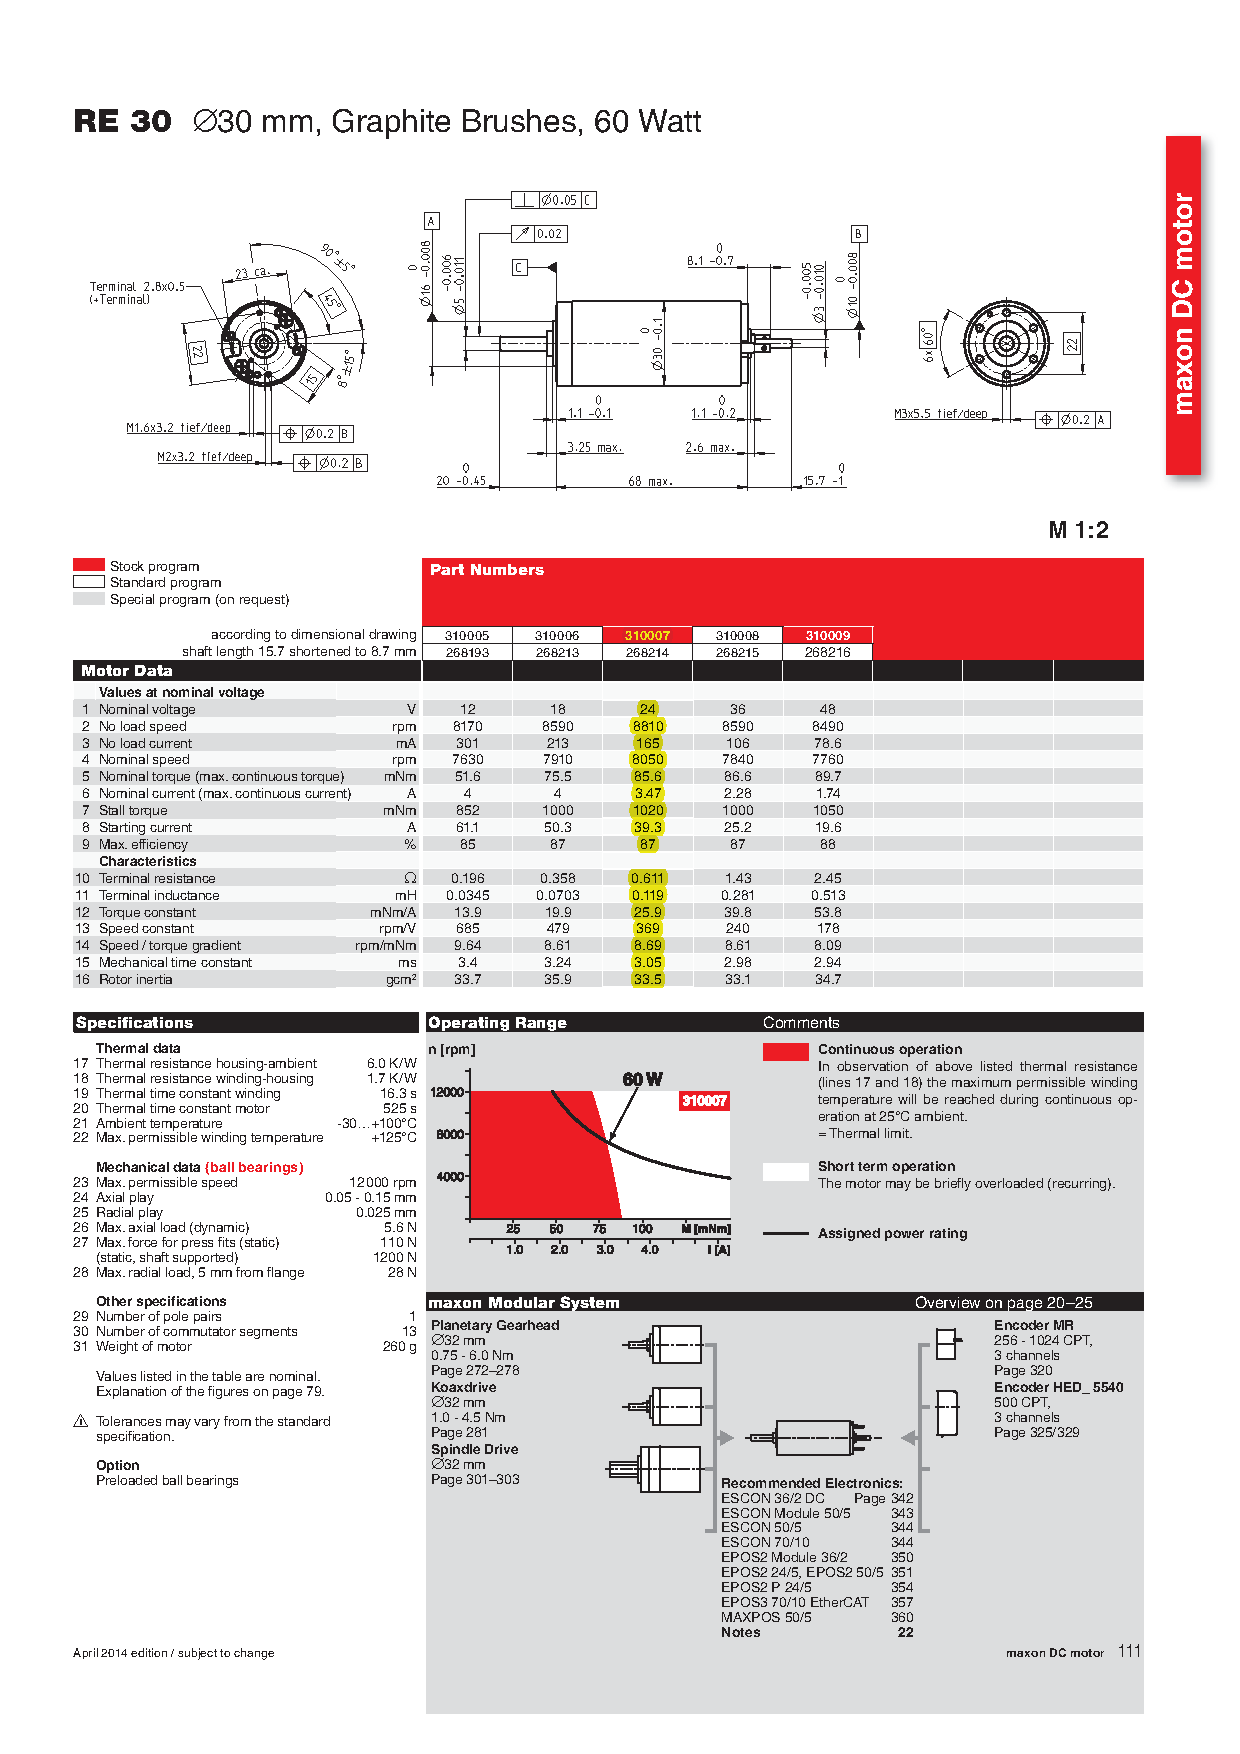
\includegraphics[page=1,width=.95\textwidth]{RE30.pdf}}
\caption{Figura ejemplo. Tomada de hoja de catálogo de \href{https://datasheets.globalspec.com/ds/17/MaxonPrecisionMotors/F1B48EDA-7358-46E6-964A-97E3BC5D921A}{motores DC con escobillas de grafito de Maxon} \copyright~2014 Maxon Motors. Reproducida con permiso.}
\label{fig:hoja-datos}
\end{figure}
	
\section{Código fuente} 
\label{sec:codigo-fuente}

Para insertar fragmentos o listados completos de código se puede usar el paquete \texttt{lstlistings}.  Permite incluir archivos o parte de archivos directamente del proyecto con la orden \texttt{lstinputlisting}.

\lstinputlisting[language=Matlab,
    caption={Ejercicio 20 como texto incorporado},
    label=src:ej20-input
]{tex/latex/ejercicio20.m}

O bien se puede copiar el texto del programa o fragmento en un entorno \texttt{lstlisting} con las mismas opciones que la orden \texttt{lstinputlisting}.

\begin{lstlisting}[language=Matlab,
    caption={Ejercicio 20 como texto en línea.},
    label=src:ej20-online
]
function [T]=Ejercicio20(f,c)

T = char('B'*ones(8,8));

for i=1:8
    for j=1:8
        if ( (i==f) || (j==c) || (i+j==f+c) || (i-j==f-c) )
            T(i,j)='*';
        elseif ( rem(i+j,2)~=0 )
            T(i,j)='N';
        end
    end
end

T(f,c)='R';
\end{lstlisting}

\info{Te recomendamos que incluyas los archivos o parte de los archivos directamente del código de tu proyecto, ya sea mediante \texttt{lstinputlisting} o mediante \texttt{inputminted}.  De esta forma mantendrás sincronizado el documento con el código fuente.}

\noindent El paquete \texttt{lstlisting} te permite quitar los números y el marco, cuando el código se incluye como parte del texto. 

\begin{lstlisting}[language=Matlab,
    frame=none,numbers=none
]
function [T]=Ejercicio20(f,c)

T = char('B'*ones(8,8));

for i=1:8
    for j=1:8
        if ( (i==f) || (j==c) || (i+j==f+c) || (i-j==f-c) )
            T(i,j)='*';
        elseif ( rem(i+j,2)~=0 )
            T(i,j)='N';
        end
    end
end

T(f,c)='R';
\end{lstlisting}

\noindent Otra forma de incluir código es mediante el entorno \texttt{verbatim}.  Este método no tiene resalte de sintaxis ni facilidades de ningún tipo para definir etiquetas o numerar las líneas. 

\begin{verbatim}
function [T]=Ejercicio20(f,c)

T = char('B'*ones(8,8));

for i=1:8
  for j=1:8
    if ( (i==f) || (j==c) || (i+j==f+c) || (i-j==f-c) )
      T(i,j)='*';
    elseif ( rem(i+j,2)~=0 )
      T(i,j)='N';
    end
  end
end

T(f,c)='R';
\end{verbatim}

\noindent Otra forma alternativa a \texttt{lstlisting} es el paquete \texttt{minted}, que colorea el programa según el lenguaje empleado.

\setminted[matlab]{
    xleftmargin=20pt,
    linenos,
    breaklines,
    bgcolor=gris85}

\begin{minted}{matlab}
function [T]=Ejercicio20(f,c)

T = char('B'*ones(8,8));

for i=1:8
    for j=1:8
        if ( (i==f) || (j==c) || (i+j==f+c) || (i-j==f-c) )
            T(i,j)='*';
        elseif ( rem(i+j,2)~=0 )
            T(i,j)='N';
        end
    end
end

T(f,c)='R';
\end{minted}

\noindent O bien, usando la orden \texttt{inputminted} para incluir directamente un archivo Matlab.

\inputminted{matlab}{tex/latex/ejercicio20.m}

}
\fi
% La bibliografía no suele ir numerada porque se pone después de los anexos.
% No se debe poner antes de los anexos porque si se cita una referencia en
% un anexo sería una backward reference, que deben evitarse a toda costa
\cleardoublepage
\hypertarget{ch:bibliografia}{%
    \printbibliography[heading=bibintoc,title={Bibliografía}]}
\cleardoublepage



\end{document}
